%
% This document is available under the Creative Commons Attribution-ShareAlike
% License; additional terms may apply. See
%   * http://creativecommons.org/licenses/by-sa/3.0/
%   * http://creativecommons.org/licenses/by-sa/3.0/legalcode
%
% Copyright 2010 Jérôme Pouiller <jezz@sysmic.org>
%

% Pour faire une version imprimable, avec les notes sans overlay
% \PassOptionsToClass{notes=show,handout}{beamer}
% Pour en faire un article:
% \documentclass[10pt,ucs,usepdftitle=false,a4paper]{article}
% \usepackage{beamerarticle}

\documentclass[10pt,ucs,usepdftitle=false]{beamer}

% Pour mettre deux pages sur une
% (Préférer l'utilisation d'un post processing)
%\usepackage{pgfpages}
%\pgfpagesuselayout{2 on 1}[a4paper,border shrink=5mm]
%\pgfpagesuselayout{4 on 1}[a4paper,landscape, border shrink=5mm]
%\setbeameroption{show notes on second screen=right}

%
% This document is available under the Creative Commons Attribution-ShareAlike
% License; additional terms may apply. See
%   * http://creativecommons.org/licenses/by-sa/3.0/
%   * http://creativecommons.org/licenses/by-sa/3.0/legalcode
%
% Copyright 2010 Jérôme Pouiller <jezz@sysmic.org>
%

% Configuration de Beamer

\usetheme{Warsaw}

% Quiris
%\usecolortheme[RGB={238,127,0}]{structure}
% Apollo
%\usecolortheme[RGB={0,56,126}]{structure}
% Sysmic
\usecolortheme[RGB={181,0,0}]{structure}

% Headers et footers
\useoutertheme[subsection=false]{smoothbars}
% Rectangle dans les itemize
\useinnertheme{rectangles}
% Pas de symboles pour la navigation
\setbeamertemplate{navigation symbols}{}

% Logo en filigranne
\setbeamertemplate{background canvas}{
  \tikz {
    \node at (0,0) {};
    \node[inner sep=0pt, opacity=0.2] at (0.5\paperwidth,-0.8\paperheight) {
\includegraphics[height=23.4mm,width=128mm]{pics/filigranne-sysmic}};
  }
}

% Ajout des numéros de pages
\newcommand*\oldinsertshortitle{}%
\let\oldinsertshorttitle\insertshorttitle%
\renewcommand*\insertshorttitle{\oldinsertshorttitle\hfill\insertframenumber\,/\,\inserttotalframenumber}

\usepackage{ucs}              % La sortie est en UTF8
\usepackage[utf8x]{inputenc}  % L'entrée aussi
\usepackage[T1]{fontenc}      % Pour la césure des mots accentués
\usepackage{lmodern}          % Pour les lettres francaises
\usepackage[french]{babel}    % Pour la sortie francaise
\usepackage{times}
\usepackage{mathptmx}         % Font (don't forget to install latex-font-recommended)

\input{style_tikz}

\ifpdf
  \usepackage{embedfile} 
\else
  \newcommand{\embedfile}[1]{}
\fi

% Produce errors like:
% main.tex:54: Undefined control sequence.
% \@EveryShipout@Output ...EveryShipout@Org@Shipout
%                                                   \box \@cclv
%\usepackage[sections,displaymath]{preview}
%\PreviewEnvironment{tikzpicture}
%\PreviewEnvironment{center}
%\PreviewEnvironment{frame}

\usepackage{hyperref} % Doit être chargé avant ntheorem
\newcommand{\email}[1]{\href{mailto:#1}{\nolinkurl{<#1>}}}
\newcommand{\man}[1]{\emph{#1}}
\newcommand{\file}[1]{\lstinline[backgroundcolor=\color{{rgb}{1,1,0.8}},language=]{#1}}
\newcommand{\cmd}[1]{\lstinline[backgroundcolor=\color{{rgb}{1,1,0.8}},language=]{#1}}
\renewcommand{\c}[1]{\lstinline[backgroundcolor=\color{{rgb}{1,1,0.8}},language=c]{#1}}

\usepackage[newcommand]{ragged2e}

% \usepackage[]{version} 
% \usepackage{ntheorem} 
% \setlength{\theorempreskipamount}{0.8ex plus 0.9ex minus 0.1ex}
% \setlength{\theorempostskipamount}{0.8ex plus 0.9ex minus 0.1ex}
% \theoremprework{\vspace{3mm}\hrule}
% \theorempostwork{\hrule\vspace{3mm}}
% \theorembodyfont{\itshape}
% \theoremseparator{.}
% \newtheorem{quest}{Question}[section]

% \theorembodyfont{\normalfont}
% \theoremseparator{}
% \theoremstyle{break}
% \newtheorem*{ans}{Réponse}

% \setlength{\theoremindent}{3mm}
% \theoremseparator{:}
% \theorembodyfont{\itshape}
% \theoremstyle{plain}
% \newtheorem*{man}{Documentation utile}
% \theorembodyfont{\normalfont}
% \newtheorem*{hint}{Remarque}
% \newtheorem*{note}{Note pédagogique}

% \usepackage[vmargin=25mm,hmargin=15mm]{geometry}          % Marges peronnalisées

% Quelques règlage de mise en page
%\renewcommand{\baselinestretch}{1.2} % taille de l'interligne
\setlength{\parindent}{0pt}
\setlength{\parskip}{0.9ex plus 0.5ex minus 0.2ex}

%\usepackage{fancyhdr}        % Fancy page headers
%\lhead{}                     % Top-Left
%\chead{}                     % Top-Center
%\rhead{}                     % Top-Right
%\lfoot{}                     % Bottom-Left
%\cfoot{}                     % Bottom-Center
%\rfoot{}                     % Bottom-Right
%\pagestyle{fancy}

\usepackage{listings}         % Pour mettre en page du code source
\usepackage{color}            % Pour les lien en couleur dans le pdf
\definecolor{colBg}        {rgb}{1,1,0.8}
\definecolor{colKeys}      {rgb}{0,0,1}
\definecolor{colComments}  {rgb}{1,0,0}
\definecolor{colString}    {rgb}{0,0.5,0}
\definecolor{colBasic}     {rgb}{0,0,0}
\definecolor{colIdentifier}{rgb}{0,0,0}
\lstset{%                     % Basic style
  numbers=left,%
  stepnumber=10,%
  numberstyle=\scriptsize,%
%
  basicstyle=\ttfamily\normalsize\color{colBasic},%
  commentstyle=\normalsize\itshape\color{colComments},%
  identifierstyle=\color{colIdentifier},%
  keywordstyle=\bf\ttfamily\color{colKeys},%
  stringstyle=\color{colString},%
  backgroundcolor=\color{colBg},%
%
%  mathescape=true,%
  extendedchars=false,%
%  tabsize=4,%
  columns=flexible,%
  fontadjust=true,%
  frame=lines,%
  showspaces=false,%
  showstringspaces=false,%
%
  emptylines=1,%
  breaklines=true,%
  breakautoindent=true,%     % Inutile avec breaklines=false
  literate={é}{{\'e}}1 {è}{{\`e}}1 {ô}{{\^o}}1 {à}{{\`a}}1 {ç}{{\c{c}}}1 
}
\lstset{language=}        % ... En C++

\definecolor{darkgreen}{rgb}{0, 0.7, 0}
\definecolor{darkgreen2}{rgb}{0, 0.5, 0}
\definecolor{red2}{rgb}{0.8, 0, 0}
\lstdefinelanguage{diff} {
    morecomment=[f][\color{darkgreen}][0]{+},
    morecomment=[f][\color{red}][0]{-},
    morecomment=[f][\itshape\color{darkgreen2}][0]{+++},
    morecomment=[f][\itshape\color{red2}][0]{---},
    moredelim=[l][\color{cyan}]{\ \@\@},
    moredelim=*[l][\color{blue}]{\@\@},
}

\hypersetup{colorlinks=true,plainpages=false,urlcolor=blue,linkcolor=}








% Apparait sur chaque slide:
%\logo{\pgfimage[height=5mm]{pics/logo}}

\title{Systèmes d'exploitation}
\hypersetup{pdftitle={Systèmes d'exploitation}}
% \subtitle{Sous-titre}
\author[Sysmic - J. Pouiller]{Jérôme Pouiller \email{j.pouiller@sysmic.org}}
\hypersetup{pdfauthor={Sysmic - Jérôme Pouiller}}
\institute[Sysmic]{}
%\institute[Sysmic]{\hspace*{1cm}\pgfimage[height=1.5cm]{pics/logo}}
% Plus complet:
% \institute[Sysmic]{
%   \inst{1} \hspace*{1cm}\includegraphics[height=1.5cm]{pics/logo}
%   \and
%   \inst{2} \includegraphics[height=1.5cm]{pics/logo-quiris}
% }
%\date[Juin 2012]{Juin 2012}
\date{}
% Pour le PDF seulement:
\subject{Systèmes d'exploitation}
\keywords{}
  
\begin{document}

  \begin{frame}[plain]
    \maketitle
    \note[item]{Parler de moi, de mon CV, freelance, sysmic, expertise, Polytech Paris, Tours, Insa Rennes}
  \end{frame}

  % -360 slides- -> 240 slides
  % 0-2 Intro, Shell (ca va déborder de 15min)
  % 2-4 Filesystems (ca va déborder de 10min)
  % 4-6 Création d'executable et les Makefile (tout juste 2h)
  % 6-8 Gestion Monotache (1h30)
  % 8-10 Gestion Multitache (2h tout juste. A étoffer)
  % 10-12 Gestion de la mémoire et debug de la mémoire(1h), Communication interprocess (A supprimer). Architecture et virtualisation (1h)

  %
% This document is available under the Creative Commons Attribution-ShareAlike
% License; additional terms may apply. See
%   * http://creativecommons.org/licenses/by-sa/3.0/
%   * http://creativecommons.org/licenses/by-sa/3.0/legalcode
%
% Created: 2012-07-28 10:50:36+02:00
% Main authors:
%     - Jérôme Pouiller <jezz@sysmic.org>
%

%\part{Introduction}

\begin{frame}[fragile=singleslide]{Programme}
  \begin{itemize}
  \item Utilisation des systèmes Unix
    \begin{itemize}
    \item Savoir utiliser l'environnement
    \item  Connaître  quelques  concepts  annexes  (file  descriptors,
      pattern matching, etc...)
    \item Rappeler les concepts de base d'un OS
    \end{itemize}
  \item Les systèmes de fichiers
    \begin{itemize}
      \item Organisation des fichiers
      \item Format des filesystems
    \end{itemize}
  \item La création d'exécutables
    \begin{itemize}
    \item La compilation
    \item Le chargement
    \end{itemize}
  \item La gestion des tâches
    \begin{itemize}
    \item Les systèmes monotâche
    \item Les systèmes multitâches
    \end{itemize}
  \item La gestion de la mémoire
    \begin{itemize}
    \item Les différents segments
    \item Les algorithmes de gestion de la mémoire
    \item Les techniques de debug
    \end{itemize}
  \item Les architectures d'OS
  \end{itemize}
\end{frame}

  %
% This document is available under the Creative Commons Attribution-ShareAlike
% License; additional terms may apply. See
%   * http://creativecommons.org/licenses/by-sa/3.0/
%   * http://creativecommons.org/licenses/by-sa/3.0/legalcode
%
% Created: 2012-07-28 10:50:36+02:00
% Main authors:
%     - Jérôme Pouiller <jezz@sysmic.org>
%

\part{Utilisation des systèmes Unix}

\begin{frame}
  \partpage
\end{frame}

\begin{frame}
  \tableofcontents
\end{frame}

\section{Le shell}

\begin{frame}[fragile=singleslide]{Historique}
  \begin{itemize}
  \item Mode de communication bas niveau privilégié
  \item  Léger,  simple  à  implémenter, puissant.   Parfois  l'unique
    manière de communiquer avec le système.
  \item Le shell ``Unix'' est plus commun. Beaucoup d'autres interface
    en ligne de commande s'en inspire.
  \item Première version du shell Unix tel qu'on le connaît écrite par
    Ken Thompson chez Bell Labs en 1971 (bien antérieur à Linux)
  \item Remplacé par le shell de Stephen Bourne en 1977
  \item  Par  ordre  approximatif d'apparition:  \cmd{sh},  \cmd{csh},
    \cmd{tcsh}, \cmd{ksh}, \cmd{bash}, \cmd{zsh}, \cmd{ash}
  \item Normalisé par la Posix 2 en 1992
  \item Fonctionne de manière plus  ou moins identique sur tous les OS
    (Linux, Androïd, iOS, Windows/Cygwin, etc...)
  \item On peut faire beaucoup de chose avec la ligne de commande
  \item Il  est possible de  faire des script  en shell. Il  arrive ce
    soir le seul langage de script disponible sur le système.
  \end{itemize}
\end{frame}

\subsection{Bases}

\begin{frame}[fragile=singleslide]{Bases de shell}
  \begin{itemize}
  \item Lancer une commande (= lancer un programme)
    \begin{lstlisting}
$ ls
    \end{lstlisting} %$
  \item Séparation des arguments par des espaces
    \begin{lstlisting}
$ mkdir dir1 dir2
    \end{lstlisting} %$
  \item Conséquence: les espaces sont des caractères spéciaux en shell
  \item  Les  arguments sont  reçus  par  le  programme par  les  deux
    arguments \c{argc} et \c{argv}
  \item  Remarque: certaines commandes  ont un  comportement différent
    suivant \c{argv[0]} (exemple: \c{test} et \c{[})
  \end{itemize}
\end{frame}

\begin{frame}[fragile=singleslide]{Convention}
  Par convention,  nous préfixons dans ces slides  les commandes shell
  par :
  \begin{itemize}
  \item  \c{$}  pour les  commandes  à  éxecuter par  l'utilisateur
    normal
  \item \c{\%} pour les commande à executer par root
  \item \c{>} pour les commandes non-shell
  \end{itemize}
\end{frame}

\begin{frame}[fragile=singleslide]{Les argument optionnels}
  \begin{itemize}
  \item Souvent les arguments optionnels commence par ``\c{-}''
  \item Les options peuvent avoir des arguments
  \item Il existe des options longues commencant par ``\c{--}''
    \begin{lstlisting}
$ ls --all
$ ls --sort=time
$ ls --sort time
    \end{lstlisting}
  \item  ... et des  options courte  tenant sur  un seul  caractère et
    commençant  par un  simple  ``\c{-}'' (attention  tout  de même  aux
    exceptions)
    \begin{lstlisting}
$ ls -l -a
$ ls
    \end{lstlisting}
  \end{itemize}
\end{frame}

\begin{frame}[fragile=singleslide]{Les argument optionnels}
  \begin{itemize}
  \item Il est possible de concaténer les option courtes
    \begin{lstlisting}
$ ls -la
    \end{lstlisting} %$
  \item Les options ne  sont \emph{normalement} pas dépendante de leur
    emplacement
    \begin{lstlisting}
$ ls -la
    \end{lstlisting} %$
  \item Ce  principe est normalisé car toutes  ces commandes utilisent
    la fonction Posix \man{getopt(3)} (mais rien ne le garanti)
  \end{itemize}
\end{frame}

%     > ls --width 60  # ok, value is "60"
%     > ls --width=60  # ok, value is "60"
%     > ls -w60        # ok, value is "60"
%     > ls -w 60       # ok, value is "60"
%     > ls -w=60       # unexpected, value is "=60"
%     > ls -T7 -w60    # ok, value for -T is 7, value for -w is 60
%     > ls -T7w60      # unexpected, value for -T is "7w60", no -w at all


\begin{frame}[fragile=singleslide]{La documentation}
  \begin{itemize}
  \item  \cmd{man  COMMAND} permet  d'accéder  à  la documentation  de
    \c{COMMAND}
  \item  Les  pages  de  man  sont  divisée  en  9  sections
  \item D'après \man{man(1)}):
    \begin{enumerate}
    \item Executable programs or shell commands
    \item System calls (functions provided by the kernel)
    \item Library calls (functions within program libraries)
    \item Special files (usually found in /dev)
    \item File formats and conventions (e.g. \file{/etc/passwd})
    \item Games
    \item  Miscellaneous (including  macro packages  and conventions),
      e.g.  \man{man(7)}, \man{groff(7)}
    \item System administration commands (usually only for root)
    \item Kernel routines [Non standard]
    \end{enumerate}
  \end{itemize}
\end{frame}

\begin{frame}[fragile=singleslide]{La documentation}
  \begin{itemize}
  \item Une même entrée peut  être présente dans plusieurs section, il
    possible de préciser la section en la plaçant en argument avant la
    commande:
    \begin{lstlisting}
$ man read
$ man 2 read
    \end{lstlisting}
  \item Les références des pages de  man sont donnés avec le numéro de
    section entre parenthèses.  Ainsi, \man{wait(2)} signifie que vous
    pouvez   accéder    à   la   documentation    avec   la   commande
    \cmd{man 2 wait}
  \item \cmd{man -l}  permet d'afficher un fichier \emph{local}
  \item \c{man man} pour plus d'information
  \end{itemize}
\end{frame}

\begin{frame}[fragile=singleslide]{Les chemins}
  Il est possible d'utiliser des chemins:
  \begin{itemize}
  \item absolus, commençant par un \c{/}
    \begin{lstlisting}
$ mkdir /tmp/tete
    \end{lstlisting}
  \item relatifs, commencant par un autre caractère
    \begin{lstlisting}
$ mkdir tmp/titi
    \end{lstlisting}
  \end{itemize}
  Les  chemins  relatifs, s'interprète  à  partir du  \emph{répertoire
    courant}  (lié au  processus actuel  et hérité  par  les processus
  fils).
  \begin{itemize}
  \item \cmd{pwd} affiche le répertoire courant
  \item \cmd{cd} modifie le répertoire courant
  \end{itemize}
\end{frame}

\begin{frame}[fragile=singleslide]{Les chemins}
  \begin{itemize}
  \item Dans un chemin, ``\c{.}'' correspond au répertoire courant
  \item ... \cmd{mkdir foo} est identique à \cmd{mkdir ././foo}
  \item ``\cmd{..}'' correspond au répertoire parent
  \item  Beaucoup de  commandes  prenant en  paramètre un  répertoire
    utilise le  répertoire courant si le paramètre  n'est pas spécifié
    (ex: \cmd{ls})
  \item  cf. \man{path\_resolution(7)}
  \end{itemize}
  Note: Les fichiers commençant  par '\c{.}' sont considérés comme des
  fichiers cachés
\end{frame}

\begin{frame}[fragile=singleslide]{Le PATH}
  % TODO: A replacer autre part
  % Normalisées par Posix, plus  ou moins regroupée dans un projet
  %  nommé coreutils
  \begin{itemize}
  \item Une commande est recherchée dans la variable \c{$PATH}
  \item  Par  défaut,   \c{$PATH}  contient  \file{/bin}  \file{/sbin}
    \file{/usr/bin} et \file{/usr/sbin}
  \item  Si  on  spécifie  le  chemin (la  commande  contient  \c{/}),
    \c{$PATH} n'est pas utilisé
  \item  Par conséquent, pour  lancer une  binaire dans  le répertoire
    courant: \cmd{./a.out}
  \item Ajouter \c{.} dans \c{$PATH} est une mauvaise pratique
  \item Mécanisme géré par la fonction Posix \man{execvpe(3)}
  \end{itemize}
\end{frame}

\begin{frame}[fragile=singleslide]{Le contenu des fichiers}
  \begin{itemize}
    \item Ne pas oublier qu'un fichier n'est qu'un vecteur d'octet
    \item Les fichiers \emph{texte} ont simplement la particularité de
      n'avoir que  des octets supérieurs  à \c{0x20} (et les  octets >
      \c{0x7F} s'interprètent  suivant la région)  (cf. \man{ascii(7)}
      et \man{charsets(7)})
    \item Le principe de ``type'' de fichier est finalement assez flou.
    \item \man{file(1)} permet de repérer le format des fichier
    \item L'utilisation d'une norme de nommage ou d'une extension peut
      aussi  aider, mais  ça  n'est  pas une  pratique  native sur  la
      plupart des OS.
    \end{itemize}
\end{frame}

\begin{frame}[fragile=singleslide]{Les file descriptor}
  \begin{itemize}
  \item  Lorsqu'un programme  souhaite  accéder à  un  fichier, il  va
    utiliser  la  fonction Posix  \man{open(3)}  qui  lui retourne  un
    nombre   appelé  \emph{file  descriptor}   (\emph{descripteur  de
      fichier}).
  \item Il s'agit d'un identifiant pour une structure dans l'OS.
  \item  Le file  descriptor peut  être passé  à d'autre  fonctions du
    système comme \man{read(3)} ou \man{write(3)}.
  \item  Nous   verrons  plus  tard  que  le   concept  de  \emph{file
      descriptor} va plus loin
  \item  Les couche basses  de l'OS  ouvre automatiquement  trois file
    descriptor lors qu'un programme est lancé:
    \begin{itemize}
    \item    Entrée    standard     (numéro    0),    accessible    en
      lecture. Normalement reliée au clavier.
    \item    Sortie    standard     (numéro    1),    accessible    en
      écriture. Normalement reliée à l'écran
    \item    Sortie    d'erreur     (numéro    2),    accessible    en
      écriture. Normalement reliée à l'écran
    \end{itemize}
  \end{itemize}
\end{frame}

\begin{frame}[fragile=singleslide]{Les redirections}
  Il est possible de demander au shell de rediriger les entrée est les
  sortie d'une commande avec les metacaractère \c{<} \c{>} et \c{|}:
  \begin{itemize}
  \item Commande standard:
    \begin{lstlisting}
$ echo foo
    \end{lstlisting}
  \item Sortie standard vers un fichier
    \begin{lstlisting}
$ echo foo > file
    \end{lstlisting}
  \item Un fichier vers l'entrée standard
    \begin{lstlisting}
$ cat -n < file
    \end{lstlisting} %$
  \item Sortie d'erreur vers un fichier
    \begin{lstlisting}
$ ls toto 2> file
    \end{lstlisting} %$
  \end{itemize}
\end{frame}

\begin{frame}[fragile=singleslide]{Les redirections}
  \begin{itemize}
  \item Sortie standard d'une commande vers l'entrée d'une autre
    \begin{lstlisting}
$ echo bar foo | wc
    \end{lstlisting}
  \item Couplage des redirections
    \begin{lstlisting}
$ cat -n < file1 | wc > file3
    \end{lstlisting} %$
  \item L'espace n'est pas obligatoire et les redirections ne sont pas
    forcement à la fin de la ligne
    \begin{lstlisting}
$ >file2 cat<file1 -n
    \end{lstlisting} %$
  \item Certaine commande detecte que la sortie est redirigée et se
    comporte différement
    \begin{lstlisting}
$ ls
$ ls | cat -n
$ ls > file
    \end{lstlisting}
  \end{itemize}
\end{frame}

\subsection{Les variables}

\begin{frame}[fragile=singleslide]{Les variables locales}
  \begin{itemize}
  \item Affectation:
    \begin{lstlisting}
$ FOO=foo
    \end{lstlisting}
  \item  Rappel: en  shell, l'espace  est un  métacaractère  donc, ces
    commandes ne fonctionnent pas:
    \begin{lstlisting}
$ FOO = foo
$ FOO=foo bar
    \end{lstlisting}
  \item Il est possible de les concaténer avec \c{+=}
    \begin{lstlisting}
$ FOO+=bar
    \end{lstlisting}
  \end{itemize}
\end{frame}

\begin{frame}[fragile=singleslide]{Les variables locales}
  La  syntaxe  \c{$\{VAR\}}  permet  de  récupérer  le  contenu  d'une
  variable.  Elle peut-être abbregée  \c{$VAR} si elle est suivit d'un
  caractère non-alphanumérique
  \begin{lstlisting}
$ echo ${FOO}
$ echo $FOO
$ echo ${FOO}_bar $FOO_bar
  \end{lstlisting}
  Sous zsh, \c{vared VAR} permet d'éditer intéractivement une variable
\end{frame}

\begin{frame}[fragile=singleslide]{Les variables d'environnement}
  \begin{itemize}
  \item   Tous  les   processus  possède   un  ensemble   de  variable
    d'envionement.
  \item  Elle   se  trouvent   dans  l'espace  mémoire   du  processus
    (cf. \man{environ(7)})
  \item   On   y    accéder   facilement   avec   \man{getenv(3)}   et
    \man{setenv(3)}
  \item  Par défaut,  un processus  hérite de  l'environnement  de son
    parent (cf. \man{execv(3)})
  \item  Un programme peut  modifier son  comportement en  fonction du
    contenu de l'environnement
  \item \cmd{export} liste les variable d'environnement
  \item \cmd{export  VAR} transforme  une variable locale  en variable
    d'environement, ou instancie la variable
  \end{itemize}
\end{frame}

\begin{frame}[fragile=singleslide]{Les variables d'environnement}
  \begin{itemize}
  \item  Il est  possible de  lancer  une commande  avec une  variable
    d'environnement particulière:
    \begin{lstlisting}
$ LANG=fr_FR.utf8 ls non-existant
ls: impossible d'accéder à  non-existant: Aucun fichier ou dossier de ce type
    \end{lstlisting}
  \item  ... ou  en utilisant  la commande  \c{env}, qui  possède plus
    d'options
    \begin{lstlisting}
$ env LANG=fr_FR.utf8 ls non-existant
ls: impossible d'accéder à  non-existant: Aucun fichier ou dossier de ce type
    \end{lstlisting}
  \item Les  variables d'environnement auront  un impact sur  tous les
    sous-processus lancés
  \item Leur  fonctionnement est  très différent des  variables shell,
    mais elle sont gérée avec la même syntaxe
  \end{itemize}
\end{frame}

\begin{frame}[fragile=singleslide]{Les variables d'environnement}
  Les variables d'environnement importantes:
  \begin{itemize}
  \item \c{PATH}: les chemins ou les commandes doivent être recherchée
  \item   \c{LANG},    \c{LOCALE}   et   \c{LC_*}:    les   information
    d'internationalisation
  \item  \c{DISPLAY}:  l'adresse  du  serveur  d'affichage  pour  les
    commande graphique
  \item \c{TERM}: le type de  terminal utilisé (nécessaire pour le bon
    affichage des couleur et des outils fenêtrés)
  \item \c{LS_COLOR}:  contient la  configuration de coloration  de la
    commande \c{ls --color}
  \item \c{PAGER}, \c{EDITOR}, \c{BROWSER}:  Les outils à utilisé pour
    visualiser, éditer et aller sur le web.
  \end{itemize}
\end{frame}

\begin{frame}[fragile=singleslide]{La syntaxe évoluée des variables}
  La syntaxe des variables peut être plus évoluée:
  \begin{itemize}
  \item  \c{$\{VAR#foo\}} ou  \c{$\{VAR/foo/bar\}} pour  effectuer des
    modification sur les variables
  \item \c{VAR=( a b c )} pour affecter un tableau
  \item \c{$\{VAR[3]\}} pour lire une value dans un tableau
  \item  Dans un  script  ou  dans une  fonction  shell, les  variable
    \c{$1}, \c{$2}, ... correspondent  aux arguments. \c{$*} et \c{$@}
    signifient ``Tous les arguments''
  \item \c{$((21 * 2))} et \c{$[43 - 1]} sont remplacé par le résultat
    de l'expression arithmétique
  \item  \c{$(echo toto)}  ou \c{`echo  toto`} sont  remplacés  par le
    résultat de la commande \c{echo toto}.
  \end{itemize}
\end{frame}

\begin{frame}[fragile=singleslide]{L'escaping}
  Sans surprise, il est  possible d'échapper un caractère spécial avec
  ``\c{\\}''
  \begin{lstlisting}
$ perl -e print\ \"Hello\ World\\n\"\;
  \end{lstlisting}
  Il est aussi possible de \emph{quoter} un argument
  \begin{itemize}
  \item Le \emph{double quote} \c{"} echappe la plupart des caractères
    sauf les variable et le \c{"} de fin:
    \begin{lstlisting}
$ perl -e "print \"Hello World\n\";"
    \end{lstlisting}
  \item Le \emph{simple quote} \c{'} échappe tous les caractères sauf le
    caractère \c{'} de fin. Il ne peux pas être échappé:
    \begin{lstlisting}
$ perl -e 'print "Hello World\n";'
    \end{lstlisting}
  \item  Le \emph{backquote}  n'est pas  un quoting,  il  correspond à
    \c{$()}
  \end{itemize}
\end{frame}

\subsection{Les patterns}

\begin{frame}[fragile=singleslide]{Le globbing}
  \begin{itemize}
  \item Langage composé de trois metacaractères:
    \begin{itemize}
    \item \c{\?}:n'importe quel caractère
    \item \c{*}: n'importe quel caractère répété 0 ou plusieurs fois
    \item  \c{[]}: N'importe  lequel des  caractère compris  entre les
      crochets
    \end{itemize}
  \item  Le shell  essaie  de faire  correspondre  tous les  arguments
    contenant ces metacaractères avec les fichier du répertoire courant
  \item ...  il remplace ensuite le  pattern par la  liste des fichier
    correspondants
    \begin{lstlisting}
$ wc -l *.c
    \end{lstlisting}
  \item Les commandes recoivent la liste des fichiers en argument, pas
    le pattern
  \item ... deux exception notables: \c{find -name} et \c{dpkg -l}. Il
    est necessaire de correctement les quoter pour que le pattern soit
    effectivement transmis à la commande
  \end{itemize}
\end{frame}

\begin{frame}[fragile=singleslide]{Les expressions régulières}
  \begin{itemize}
  \item Ressemble de loin au globbing
  \item Plus de metacaractères:
    \begin{itemize}
    \item \c{.}: N'importe quel caractère
    \item \c{[]}:  N'importe lequel  des caractères contenu  entre les
      crochets
    \item \c{*} Le caractère précédants répété 0 ou plusieurs fois
    \item \c{+} Le caractère précédant répété 1 ou plusieurs fois
    \item \c{\{X,Y\}} Le caractère précédant répété entre X et Y fois.
    \item  \c{()} Mémorise  un  groupe qui  peut  être référencé  avec
      \c{\\X}
    \item \c{^} \c{$} Début et fin de ligne
    \end{itemize}
  \item ... voir \man{regex(7)} pour la spécification complète
  \end{itemize}
  Ainsi:
  \begin{itemize}
  \item \c{^a.*b.*$} matche avec \c{a123b45}
  \item \c{^a(.)*b\1$} matche avec \c{a1111b1}
  \end{itemize}
\end{frame}

\begin{frame}[fragile=singleslide]{Les expressions régulières}
  \begin{columns}
    \begin{column}{6cm}
      \begin{itemize}
      \item D'un  point de vu  formel, les expressions  régulières peuvent
        décrire des grammaires régulières (de Type 3 dans la hiérarchie de
        Chompsky)
      \item Il  est possible de  démontrer qu'il est existe  une bijection
        entre  l'ensemble  des  expressions  régulière et  l'ensemble  des
        automates à état fini
      \item A titre de comparaison, Bison est un outils capable d'exprimer
        des grammaires de Type 2 (dite \emph{context-free})
      \end{itemize}
    \end{column}
    \begin{column}{4cm}
      \includegraphics[height=7cm]{pics/HierarchieChomsky}
    \end{column}
  \end{columns}
\end{frame}

\begin{frame}[fragile=singleslide]{Les expressions régulières}
  Les deux implémentations de  moteur d'expression régulières les plus
  répandues  sont celles  de  GNU (Gnu  Regular Expression  Processor,
  \man{grep(1)}) et de Perl (\man{perlreref(3)}).
  \begin{lstlisting}
$ echo a123b45 | grep -E '^a.*b.*$'
a123b45
$ echo a1111b1 | perl -ne 'print if /^a(.)*b\1$/;'
a1111b1
  \end{lstlisting}
  \begin{itemize}
  \item Il  peut exister des différences entre  les implémentations de
    Perl et de \cmd{grep}
  \item  Beaucoup de  commande  prennent des  expression régulière  en
    entrée. Attention à  ce qu'elle ne soit pas  interprétées comme du
    globbing par le shell
  \item Les expressions régulières, c'est bon, mangez-en.
    % TODO  faire un slide entier  d'exemple d'expressions régulières,
    % avec matching de fonction C, d'IP, etc...
  \end{itemize}
\end{frame}

\begin{frame}[fragile=singleslide]{Exemples}
  Exemples:
  \begin{itemize} 
%  \item \verb+^[ \t]*\$+: Lignes vides
%  \item            \verb+([0-9]{1,3}\.){3}[0-9]{1,3}+           (PCRE:
%    \verb+(\d{1,3}\.){3}\d{1,3}+): IP
  \item          \verb+[a-zA-Z]*://[a-zA-Z0-9_/%\.-]*+          (PCRE:
    \verb+\w*://\S*+): URL
  \item \verb+^[a-zA-Z_].*\)[^;]*\$+: Définitions de fonctions C
  \end{itemize} 
\end{frame} 

\begin{frame}[fragile=singleslide]{Outils dérivés}
  Quelques outils pour travailler avec les expression régulières
  \begin{itemize}
  \item  \cmd{ed}, \cmd{grep},  \cmd{sed}, \cmd{awk},  \cmd{perl -pe}:
    Outils de traitement de texte automatique
  \item \cmd{ed}, \cmd{ex}, \cmd{vi}, \cmd{vim}: Editeurs de texte
  \end{itemize}
\end{frame}

\subsection{Quelques sujets plus avancés}

\begin{frame}[fragile=singleslide]{Le terminal}
  \begin{itemize}
  \item Lourd historique
  \item  Il existe(ait)  énormément de  terminaux  différents. Chaque
    terminal à ses spécificités:
    \begin{itemize}
    \item caractère permettant le retour à la ligne,
    \item possibilité de déplacer le curseur,
    \item possibilité de souligner,
    \item de mettre des caractères en gras,
    \item terminaux en couleur,
    \item  séquence retournée  par les  touches  spéciales (backspace,
      delete, flèche, touches de fonction, composition de touches,...)
    \end{itemize}
  \item Le minitel est(était) un terminal compatible VT102
  \end{itemize}
\end{frame}

\begin{frame}[fragile=singleslide]{Le terminal}
  \begin{itemize}
  \item   Les   terminaux  virtuel   choisissent   quelle  norme   ils
    implémentent (il peuvent en faire une nouvelle)
  \item La variable d'environnement \c{$TERM} indique aux commandes le
    type de terminal. De nos jours, la valeur \c{xterm} est de loin la
    plus répandue.
  \item \c{<Ctrl+V>} permet d'afficher la séquence de touche recue par
    le shell sans l'interpréter
  \item Les couleurs  se font avec des séquence  d'échappement plus ou
    moins  standardisée (Norme ECMA-48):  \c{\x1B[32m} pour  le rouge,
    etc...  (cf \man{console\_codes(4)})
  \item  La bibliothèque  \c{readline}, très  largement  utilisée gère
    tout  cet aspect.   \c{readline} inclut  une base  de  données des
    fonctionnalités de tous les terminaux existants
  \item Exception notable à  cette norme: Les systèmes d'exploitations
    de Microsoft  (il est possible  de commander le terminal  avec des
    appels systèmes)
  \end{itemize}
\end{frame}

\begin{frame}[fragile=singleslide]{Jobs control}
  \begin{itemize}
  \item  Il est  possible de  travailler avec  plusieurs  commandes en
    parallèles
  \item \c{<CTRL+Z>}  suspend la commande courante. En  fait, c'est le
    noyau qui transforme cette combinaison  de touche en signal et qui
    suspend le programme si celui-ci lui permet.
  \item    \c{fg}   continue   l'éxecution    de   la    commande   en
    \emph{foreground}
  \item    \c{bg}   continue   l'éxecution    de   la    commande   en
    \emph{background}
  \item  Il  est  possible  de  lancer  une  commande  directement  en
    backgound en la terminant pas \c{&}
  \item \c{jobs} liste les jobs en cours d'éxection
  \end{itemize}
  \begin{lstlisting}
$ cp -r bigdir newdir
<CTRL+Z>
$ sleep 100 &
$ jobs
[1]  - suspended  cp -r bigdir newdir
[2]  + running    sleep 100
  \end{lstlisting}
\end{frame}

\begin{frame}[fragile=singleslide]{Ecrire des scripts}
  \begin{itemize}
  \item Les scripts possèdent la même syntaxe que la ligne de commande
  \item  Commencent  par  le   chemin  de  l'interpréteur  prefixé  de
    ``\c{#!}''
    \begin{lstlisting}
#!/bin/sh
#!/usr/bin/perl
#!/bin/sed
#!/usr/bin/make -f
    \end{lstlisting}
  \item L'OS appelle l'interpreteur et  passe le fichier de script et
    ses   arguments   en  paramètres.   (Essayez   avec  votre   propre
    application)
  \item Il  est possible  de les lancer  en les passant  directement à
    l'interpreteur de commande
  \item Doivent avoir les droits en execution
    \begin{lstlisting}
$ bash script.sh
$ chmod +x script.sh
$ ./script.sh
    \end{lstlisting} %$
  \end{itemize}
\end{frame}

\begin{frame}[fragile=singleslide]{Ecrire des scripts}
  \begin{itemize}
  \item Il est bien sur possible d'appeller d'autres scripts
  \item Il est possible de sourcer d'autres script (!= appeller)
    \begin{lstlisting}
source lib.sh
. lib.sh
    \end{lstlisting}
  \item Il est possible de déclarer des fonctions
    \begin{lstlisting}
function bar {
}
foo() {
}
    \end{lstlisting}
  \end{itemize}
\end{frame}

\begin{frame}[fragile=singleslide]{Ecrire des scripts}
  \begin{itemize}
  \item Il est possible de séparer deux commandes par \c{\;}
  \item La commande \man{test(1)} (ou \man{[(1)}) permet d'interpréter
    des conditions
  \item Il existe aussi des structures de contrôle:
    \begin{lstlisting}
if test -n $VAR; then
  echo '$VAR exist'
else
  echo '$VAR does not exist'
fi
while [ -z $VAR ]; do
  VAR+=$(cat file)
done
    \end{lstlisting}
  \end{itemize}
\end{frame}

\begin{frame}[fragile=singleslide]{Quelques derniers trucs}
  \begin{itemize}
  \item En  début d'argument  \c{\~/} sera remplacé  par Le  chemin de
    votre \emph{home}
  \item  La syntaxe \c{a\{1,2\}b}  sera remplacé  par \c{a1b  a2b}. Ca
    n'est pas  du globbing,  car ca ne  matche pas avec  le répertoire
    courant
  \item Complétion
    \begin{lstlisting}
$ cd /h<TAB>/j<TAB>/c<TAB>
    \end{lstlisting}
  \item Les  shell modernes sont  capables de faire de  la completion
    avancée
    \begin{lstlisting}
$ man l<TAB>
    \end{lstlisting}
  \end{itemize}
\end{frame}

\begin{frame}[fragile=singleslide]{Quelques derniers trucs}
  \begin{itemize}
  \item Alias
    \begin{lstlisting}
$ alias ll="ls -l --color=auto"
$ alias cp="cp -i"
$ alias mv="mv -i"
$ alias rm="rm --one-file-system"
    \end{lstlisting} %$
  \item Il est possible  de mettre des commande dans \file{\~/.bashrc}
    ou  \file{\~/.zshrc} qui  seront  éxecutée à  chaque démarrage  du
    shell.
  \item Man de la commande courante (sous Zsh uniquement)
    \begin{lstlisting}
$ rm -<M-h>
    \end{lstlisting} %$
  \end{itemize}
\end{frame}

\begin{frame}[fragile=singleslide]{Travailler réseau en deux mots}
  \begin{itemize}
  \item  \cmd{/sbin/ifconfig  -a} donne  la  configuration des  cartes
    réseaux
  \item \c{lo} correspond à la carte réseau virtuelle de localhost
  \item \cmd{route -n} affiche la table de routage du système (kernel)
  \item     \file{/etc/resolv.conf}    et    \file{/etc/nsswitch.conf}
    contiennent la configuration du service de résolution de nom (dont
    le DNS) (libc)
  \item  ... de  nos jours,  on  utilise souvent  un proxy  DNS et  la
    configuration       du       DNS       se      retrouve       dans
    \file{/var/run/nm-dns-dnsmasq.conf}
  \item \cmd{iptables} gère les règle de filtrage
  \item Bien  que très utilisée, ces commandes  peuvent être remplacée
    par iproute2 (et sa cmmande \c{ip})
  \item \cmd{netstat -n} ou  \cmd{netstat -ln} permet d'obtenir l'état
    des connexions réseaux
  \end{itemize}
\end{frame}

\section{Un shell à distance}

\begin{frame}[fragile=singleslide]{Travailler à distance}
  Protocoles les plus utilisés:
  \begin{itemize}
  \item Telnet
    \begin{itemize}
    \item \cmd{telnetd} et \cmd{telnet}
      \begin{lstlisting}
host$ telnet -l root target
target%
      \end{lstlisting} %$
    \item   Pas   sécurisé,   attention   a   votre   mot   de   passe
      \note[item]{faire    une   démonstration    avec    telnetd   et
        \cmd{tcpdump  -i  lo -A  port  telnet}  (il  faut regarder  le
        dernier caractère de chaque paquet envoyé)}
    \item \verb/<CTRL+]>/ permet d'accéder à l'interface de commande
    \end{itemize}
  \item Ssh
    \begin{itemize}
    \item \cmd{sshd} et \cmd{ssh}
      \begin{lstlisting}
host$ ssh root@target
target%
      \end{lstlisting} %$
    \item Sécurisé
    \item Pleins de bonus de sécurisé
    \item   Il   est   possible   de  forcer   la   déconnexion   avec
      \verb/<RET><~><.>/   et   de   suspendre  une   connexion   avec
      \verb/<RET><~><CTRL+Z>/
    \end{itemize}
  \end{itemize}
\end{frame}

\subsection{Utilisation de clefs numériques}

\begin{frame}[fragile=singleslide]{Utiliser des clef ssh}
  \begin{itemize}
  \item Possibilité de créer des clefs pour \cmd{ssh}
    \begin{lstlisting}[language=sh]
host$ ssh-keygen -t dsa
    \end{lstlisting} %$
  \item Toujours mettre un mot de passe sur votre clef
  \item Recopiez votre clef dans \verb+~/.ssh/authorized_keys+
    \begin{lstlisting}[language=sh]
host$ ssh-copy-id root@target
    \end{lstlisting} %$
  \end{itemize}
\end{frame}

\begin{frame}[fragile=singleslide]{Utiliser des clef ssh}
  \begin{itemize}
  \item Utiliser ssh-agent
    \begin{lstlisting}[language=sh]
host$ ssh-agent
host$ SSH_AUTH_SOCK=/tmp/agent.3391; export SSH_AUTH_SOCK;
host$ SSH_AGENT_PID=3392; export SSH_AGENT_PID;
host$ echo Agent pid 3392;
    \end{lstlisting} %$
  \item Enregistrer votre passphrase auprès de l'agent
    \begin{lstlisting}[language=sh]
host$ ssh-add
    \end{lstlisting} %$
  \item Forwarder votre agent
    \begin{lstlisting}[language=sh]
host$ ssh -A root@target
target%
    \end{lstlisting} %$
  \end{itemize}
\end{frame}

\begin{frame}[fragile=singleslide]{Forwarder des ports}
  \begin{itemize}
  \item \c{ssh  -L 1080:far-far-host:80 far-host}: Une  demande sur le
    port 1080  de ma machine  \c{locale} est forwarder  à \c{far-host}
    qui se connecte sur \c{far-far-host} sur le port 80. Très utile si
    far-far-host n'est pas directment accessible par internet.
  \item  \c{ssh -R  1080:close-host:80 far-host}:  Une demande  sur le
    port 1080  de \c{far-host} est  forwarder à ma  machine \c{locale}
    qui se connecte  sur \c{close-host} sur le port  80. Très utile si
    je dois acceder à \c{close-host} à partir de far-host
  \item  \c{ssh  -D  1080  far-host}  Idem  que  l'option  \c{-L}.  En
    revanche, je  peux demander à  crée un tunnel vers  n'importe quel
    host  dynamique. On  utilise le  protocole socks  utilisé  par les
    proxy. Certaine commande intègre  le gestion de ce protocole. Pour
    les autre, on peut utiliser \man{socksify(1)}
  \item L'étape  suivante est de créer une  interface réseau virtuelle
    passant par  ce canal et de  lui affecter des  route. On obtenient
    ainsi un VPN.
    \item cf. \man{ssh(1)}
  \end{itemize}
\end{frame}

\section{Les droits}

\begin{frame}[fragile=singleslide]{Les utilisateurs}
  \begin{itemize}
  \item Il  y a plusieurs utilisateurs  sur le système.  Il sont gérés
    dans \file{/etc/passwd}
  \item Il y a des groupe sur le système, gérés dans \file{/etc/group}
  \item  Une  utilisateur  peur  appartenir  à  plusieurs  groupes  et
    plusieurs utilisateurs peuvent appartenir au même groupe
  \item Ces utilisateurs  et ces groupes sont gérés avec  leurs UID et leurs
    GID, \file{/etc/passwd} et  \file{/etc/group} s'occupent de faire
    la correspondances avec les nom lors de l'affichage
  \item \emph{root} (UID 0) est l'utilisateur privilégié
  \item Certaine  fonction ne peuvent  être exécuté que par  root (par
    exemple: modifier l'horloge, la configuration réseau)
  \item Il existe plusieurs manières pour devenir \c{root}
    \begin{itemize}
    \item \c{login}
    \item \c{su}
    \item \c{sudo}
    \end{itemize}
  \item Chaque fichier  du système est associé à  un propriétaire et à
    un groupe
  \end{itemize}
\end{frame}

\begin{frame}[fragile=singleslide]{Principes de base des mots de passe}
\begin{itemize} 
\item Les mots de passe stockés en clair ne sont pas une bonne idée
  \begin{itemize}
  \item time attack 
  \item problème de l'utilisation du  même mot de passes sur plusieurs
    systèmes   (peuvent être   utilisé   par  un   attaquant  ou   par
    l'administrateur)
  \end{itemize} 
\item Les  mots de passe  se trouvent dans \file{/etc/passwd}  ou dans
  \file{/etc/shadow}
\item Si champ est vide, il est permis de se logger sans mot de passe
\item  On encode  les mots  de passe  avec un  algorithme non-reversif
  (type hash)
\item  Lorsqu'on vérifie  le  mot  de passe,  on  compare les  version
  encodée
\item Il est difficile de retrouver le mot de passe d'origine à partir
  du mot de passe codé.
\end{itemize}
\end{frame}

\begin{frame}[fragile=singleslide]{Principes de base des mots de passe}
\begin{itemize} 
\item En revanche, il n'est  pas forcément nécessaire d'avoir le mot de
  passe en clair. On ajoute donc du sel au mot de passe:
\begin{lstlisting} 
$ mkpasswd -m des foo ab
abQ9KY.KfrYrc
$ mkpasswd -m des foo cd
cdEPlIkpb3972
\end{lstlisting} 
\item Le fichier  \file{/etc/passwd} contient es information obligeant
  à  laisser les  droits en  lecture à  tous les  utilisateurs  sur ce
  fichier.
\item  De plus, le  format du  fichier \file{/etc/passwd}  n'était pas
  prévu pour être extensible.
\item   On   a   alors    crée   un   nouveau   format   de   fichier:
  \file{/etc/shadow}.  Celui-ci accepte plusieurs algorithmes.
\begin{lstlisting} 
mkpasswd -m sha-512 foo abcdefgh
$6$abcdefgh$j0MVxgmPHdViHdU0fAVeXckk8X1/N...
\end{lstlisting}
\item Les systèmes à mots de passe restent relativement peu sécurisé à
  partir du moment ou l'attaquant récupère la version crypté du mot de
  passe.
\end{itemize} 
\end{frame}

\begin{frame}[fragile=singleslide]{Les droits}
  \begin{itemize}
  \item  Chaque fichier  possède  3 +  3  x 3  droits (modifiable  par
    \man{chmod(1)}):
    \begin{itemize}
    \item \c{w}: Ecriture
    \item \c{r}: Lecture: Pour un répertoire, cela permet de lister le contenu
    \item \c{x}: Execution: Pour un fichier cela permet de
      l'éxecuter. Pour un répertoire, cela permet d'accéder au
      fichiers contenus dans le répertoire.
    \end{itemize}
  \item Ces trois droits sont répétés pour
    \begin{itemize}
    \item \c{u}: Le propriétaire
    \item \c{g}: Le groupe
    \item \c{o}: Le reste du monde
    \end{itemize}
    \begin{lstlisting}[columns=fixed]
$ ls -ld /bin/ls ~/.bashrc
-rwxr-xr-x  1 root root   [...] /bin/ls
-rwxrwxrwx  1 jezz jezz   [...] /home/.bashrc
    \end{lstlisting}
  \item Il est  pratique d'écrire ses droit sous  la forme octal: 755,
    644, etc...
  \end{itemize}
\end{frame}

\begin{frame}[fragile=singleslide]{Les droits}
  \begin{itemize}
  \item Il existe en plus:
    \begin{itemize}
    \item SetUid/SetGid (ex: \cmd{ping}): La commande prend les droits
      du propriétaire/groupe lorsqu'elle s'éxecute
    \item Sticky Bit  (ex: \cmd{/tmp/}): Il est possible  de créer des
      fichier mais, seul le propriétaire du fichier peut l'effacer.
    \end{itemize}
    \begin{lstlisting}[columns=fixed]
$ ls -ld /tmp /bin/ping
-rwsr-xr-x  1 root root   [...] /bin/ping
drwxrwxrwt 13 root root   [...] /tmp
    \end{lstlisting}
  \item Il  existe des système de  gestion de droits  plus fin (Access
    Control List), mais pas aussi utilisé.
  \end{itemize}
\end{frame}

\section{Gestion de fichiers systèmes}

\begin{frame}[fragile=singleslide]{Gestion des paquets}
  \begin{itemize}
  \item La principale  raison obligeant à être root  pour installer un
    paquet est pour écrire les répertoires appartenant à root.
  \item Un  programme est livré  sous forme d'un paquet  contenant: la
    binaire, la documentation et les éventuelles ressources
  \item Il s'agit ni plus  d'une tarball (\c{tar} est utilisé dans les
    \c{.deb} alors que \c{cpio} est utilisé dans les \c{.rpm}).
  \item  Lors de  la décompression  (\c{dpkg -i},  \c{rpm  -i}, \c{ipk
      -i}),  on écrit dans  une base  de donnée  les nom  des fichiers
    décompressé afin de pouvoir facilement supprimer le paquet
  \item On  ajoute un fichier  normalisé à cette tarball  afin d'avoir
    des informations supplémentaires:
    \begin{itemize}
    \item Version
    \item Description
    \item Dépendances
    \item Signature
    \item ...
    \end{itemize}
  \end{itemize}
\end{frame}

\begin{frame}[fragile=singleslide]{Gestion des paquets}
  \begin{itemize}
  \item On  peut interroger  la base de  donnée des  fichier installés
    avec (\c{dpkg -l}, \c{dpkg -L}, \c{dpkg -S}, \c{rpm -q})
  \item Afin  de ne pas devoir récupérer  chaque paquets manuellement,
    on  crée des  dépôts  centralisé et  indexé.   Des outils  peuvent
    interroger ces  bases (\c{apt-get}, \c{urpmi},  \c{yum}, ...).  il
    peuvent  automatiquement  récupérer  les  dépendance  et  appeler
    \c{dpkg}/\c{rpm}
  \item Lors  de l'installation,  on note si  le paquet a  été demandé
    explicitement   ou  si   il   a  été   installé   à  cause   d'une
    dépendance.  Lorsqu'un  paquet  n'a  plus d'utilité,  on  peut  le
    désinstaller automatiquement.
  \item     Pleins    d'autres    outils     utiles:    \c{apt-cache},
    \c{apt-get source}, \c{apt-get  source -b}, \c{apt-get builddeps},
    etc...
  \end{itemize}
\end{frame}
 % 4h
  %
% This document is available under the Creative Commons Attribution-ShareAlike
% License; additional terms may apply. See
%   * http://creativecommons.org/licenses/by-sa/3.0/
%   * http://creativecommons.org/licenses/by-sa/3.0/legalcode
%
% Created: 2012-07-28 20:09:12+02:00
% Main authors:
%     - Jérôme Pouiller <jezz@sysmic.org>
%

\part{Les systèmes de fichiers}

\begin{frame}
  \partpage
\end{frame}

\begin{frame}
  \tableofcontents[currentpart]
\end{frame}

\section{L'arborescence}

\begin{frame}[fragile=singleslide]{Généralités}
  Les types de fichiers
  \begin{itemize}
  \item Normal (\man{touch(1)}, \man{open(2)}, \man{mknod(2)})
  \item Répertoire (\man{mkdir(1)}, \man{mkdir(2)})
  \item Lien symbolique (\man{ln(1)}, \man{symblink(2)})
  \item Pipe nommé (\man{mkfifo(1)}, \man{mkfifo(3)}, \man{mknod(2)})
  \item Socket nommé (\man{bind(2)}, \man{mknod(2)})
  \item     Fichier    périphérique     charactère    (\man{mknod(1)},
    \man{mknod(2)})
  \item Fichier périphérique bloc (\man{mknod(1)}, \man{mknod(2)})
  \end{itemize}

  Par ailleurs, il  est possible de faire pointer  une nouvelle entrée
  vers une  structure de fichier existante.  Ce  mécanisme est appellé
  \emph{hard link}  (\man{ln(1)}, \man{link(2)}). Certain  système COW
  fonctionnes ainsi.
  \\
  Tous les caractères sont  autorisés sauf \c{/} (réservé pour séparer
  les  répertoires)  et \c{\\0}  (réservé  pour  indiquer  la fin  des
  arguments)
\end{frame}

\begin{frame}[fragile=singleslide]{Arborescence}
  Il s'agit  d'un standard, pour les systèmes  spécialisé, beaucoup de
  ces répertoire n'existeront pas.

  \man{debootstrap(1)} permet de crée une nouvelle arborescence et d'y
  décompresser   les   fichiers   minimum  au   fonctionnement   d'une
  distribution Debian

  Lorsque  vous  installez  (ou   compilez)  un  paquet,  vous  pouvez
  spécifier de l'installer à partir d'une autre racine.

  %   Peut-etre    à   mettre   dans   la   partie  virtualisation?
  Il  est possible  de s'exécuter  sur une  autre racine  à  l'aide de
  \man{chroot(1)}
\end{frame}

\begin{frame}[fragile=singleslide]{Arborescence}
  \begin{itemize}
  \item  \file{/bin}  \file{/sbin}  \file{/usr/bin}  \file{/usr/sbin}:
    Binaires
  \item \file{/} et \file{/usr} séparé pour des raison historiques
  \item \file{*/sbin}: Binaire normalement réservée à root
  \item \file{/lib*} \file{/usr/lib*}: Bibliothèque
  \item \file{/etc}:  Fichiers de configuration  système.  Beaucoup se
    terminent en \file{*rc.conf}
  \item \file{/home}, \file{/root} Espace des utilisateurs
  \end{itemize}
\end{frame}

\begin{frame}[fragile=singleslide]{Arborescence}
  \begin{itemize}
  \item \file{/var} Répertoire de travail des applications systèmes
  \item \file{/var/spool} Queue de traitement de certains démon (mail,
    imprimante, etc...)
  \item \file{/var/log} Logs système
  \item \file{/var/cache}  Cache système de certains  outils (index de
    man, version binaire des index apt, debconf, etc...)
  \item \file{/var/run} et  \file{/run} Fichier de communication entre
    les services  (fichiers de lock, PIDs,  sockets des communication,
    identifiants de mémoire partagée, etc...)
  \item  \file{/var/lib} Données de  travail de  certaine bibliothèque
    (apt, ...)
  \item \file{/var/www}, \file{/var/mail},  ...  Dédié aux partage web
    et mails
  \end{itemize}
\end{frame}

\begin{frame}[fragile=singleslide]{Arborescence}
  \begin{itemize}
  \item  \file{/usr/share}  Donnée   statiques  de  certains  services
    (icônes,  fonts,  internationalisation, configurations  statiques,
    etc...)
  \item \file{/usr/share/man} Pages de man
  \item \file{/usr/share/doc} Autre documentation, Licences
  \item  \file{/usr/include}  Fichiers  entêtes  des  bibliothèques  C
    (installés par les version \c{*-dev} des packets)
  \item \file{/usr/local} \file{/opt}  Application installée en dehors
    du service de packets normal (compilés localement)
  \item      \file{/tmp}       et      \file{/var/tmp}      Répertoire
    temporaire. \file{/tmp} est vidé à chaque redémarrage
  \end{itemize}
\end{frame}

\begin{frame}[fragile=singleslide]{Le répertoire \file{/dev}}
  \begin{itemize}
  \item Fichiers spéciaux, \emph{file devices}
  \item Communiquent avec des drivers (sous Unix, tout est fichier)
  \item \man{dd(1)}  permet un contrôle  plus fin et est  souvent plus
    approprié  que  \emph{cat}  et  \emph{echo}  pour  accéder  à  ces
    fichiers
  \item Certains  périphérique nécessite l'utilisation  d'autre appels
    système qui nous verrons plus tard
  \item Dans  tous les cas,  ces appels systèmes passent  utilisent un
    file descriptor comme identifiant
  \end{itemize}
\end{frame}

\begin{frame}[fragile=singleslide]{Le répertoire \file{/dev}}
  Quelques exemples:
  \begin{itemize}
  \item \file{/dev/ttyS0}: Premier port série
  \item \file{/dev/sda}: Premier disque
  \item \file{/dev/sr0}: Lecteur CD
  \item \file{/dev/mem}: Mémoire physique
  \item \file{/dev/zero}: Périphérique virtuel qui ne donne que des 0
  \item \file{/dev/random}: Source d'entropie
  \item \file{/dev/null}: Trou noir
  \item   \file{/dev/psaux}   et  \file{/dev/input/*}:   Périphériques
    d'entrées (souris, clavier, touchsreen, etc...)
  \item \file{/dev/snd/}: Cartes son
  \item \file{/dev/rtc0}: Horloge (plus spécial à accéder)
  \item \file{/dev/video0}, \file{/dev/nvidia}: Webcam, carte vidéo ne
    s'accèdent pas directement (nous y reviendrons)
  \end{itemize}
\end{frame}

\begin{frame}[fragile=singleslide]{Le répertoire \file{/dev}}
  N'apparaissent pas:
  \begin{itemize}
  \item Les bus (cas très rare et anormaux ou on fait des implémentations
    en userland),
  \item Les cartes  et les périphériques réseaux (à  l'heure du cloud et
    des environnement distribué, ca peut avoir son importance)
  \item  Les cartes  vidéo n'apparaissent  pas toujours.  Certains driver
    sont implémentés en userspace
  \end{itemize}
\end{frame}


\subsection{Les filesystems}

\begin{frame}[fragile=singleslide]{Les filesystems}
  \begin{itemize}
  \item Une  partition de disque est \emph{montée}  sur un \emph{point
      de montage}
  \item Un point de montage est un répertoire (vide de préférence)
  \item \man{mount(1)} \man{mount(2)} \man{mount(8)}
  \item  Il  existe  différent  type  de file  systemes:  vfat,  ntfs,
    iso9660, ext2, ext3, ext4, xfs, btrfs, reiserfs, cramfs, squashfs,
    jffs2
  \item  Il est  possible de  monter  un fichier  normal plutôt  qu'un
    fichier périphérique  avec \cmd{-o loop} (une image  disque ou une
    iso par exemple)
  \item \c{tmpfs} est mappé de sur de la mémoire RAM
  \item \c{procfs}  (monté sur  \file{/proc}) et \c{sysfs}  (monté sur
    \file{/sys}) sont des file systems virtuels
  \item Il permettent d'obtenir des informations sur l'état du noyau.
  \item Filesystems réseau: nfs, samba
  \item Filesystems plus complexes, implémenté en userland par FUSE (à
    l'aide de \file{/dev/fuse}): sshfs, ftpfs, etc..
  \end{itemize}
\end{frame}

\section{Implémentations}

\begin{frame}[fragile=singleslide]{Table des partitions}
  \begin{columns}
    \begin{column}{8cm}
      \begin{itemize}
      \item Inventée par Microsoft à peu près en même temps que la FAT
      \item CHS (Cylindre-Head-Sector) est  obsolete, de nos jours, on
        accède  au  disque  en   utilisant  leur  LBA  (Logical  Block
        Addressing)   (les  disque   IDE  doivent   implémenter  cette
        compatibilité, je ne crois pas que ca soit encore présent dans
        le protocole sata )
      \item Les 512 premiers octets représente la table
      \item Les 446 premiers octets contiennent le \emph{Bootcode} (un
        boot  loader s'appuyant  sur  le bios  encore  utilisé de  nos
        jours)
      \item Ensuite un tableau de  4 entré de 16 octets représentation
        4 partitions principales
      \item Chaque  entré contient le type, l'adresse  (LBA) de départ
        et la taille de la partition (répété dans le filesystem)
      \end{itemize}
    \end{column}
    \begin{column}{4cm}
      \includegraphics[height=5cm]{pics/mbr}
    \end{column}
  \end{columns}
\end{frame}

\subsection{VFAT}

\begin{frame}[fragile=singleslide]{Vfat}
  \begin{columns}
    \begin{column}{7cm}
  \begin{itemize}
  \item Acronyme de File Allocation Table
  \item Inventé par Microsoft en 1977
  \item Disque divisé en cluster de  $512 * 2^n$ octets (en fait $2^n$
    \emph{secteurs} de 512 octets)
  \item  La structure  volume ID  est  placée à  l'adresse zéro,  elle
    contient la taille des  cluster, l'adresse du répertoire racine et
    la taille de la FAT (nous  verrons que la taille de la partition =
    taille de fat en double mots * taille du cluster en octets)
  \end{itemize}
    \end{column}
    \begin{column}{5cm}
      \includegraphics[height=5cm]{pics/volume_id}
    \end{column}
  \end{columns}
\end{frame}

\begin{frame}[fragile=singleslide]{Les répertoires}
  Les répertoires
  \begin{itemize}
  \item Un  cluster répertoire est  un vecteur de  structures pointant
    sur des fichiers ou d'autres répertoire.
  \item Les entrée  contiennent un plus des information  comme le nom,
    la taille et les attribut des fichiers
    \begin{center}
      \includegraphics[height=0.8cm]{pics/dir_entry_short}
    \end{center}
  \item  Il existe  des valeurs  spéciales pour  indiquer  les entrées
    supprimées et la fin du listing
  \item On peut ainsi parcourir les fichier du disque
  \end{itemize}
\end{frame}

\begin{frame}[fragile=singleslide]{La FAT}
  Et si le fichier ou le répertoire ne tient pas sur un cluster?
  \begin{columns}
    \begin{column}{7cm}
      \begin{itemize}
      \item La FAT intervient
      \item La FAT est un tableau de d'entiers de 32bits (ou 16bits ou
        12 bits)
      \item Chaque  entrée représente un cluster (entrée  1 == cluster
        1)
      \item  Si  l'entrée  vaut  0,  le cluster  est  disponible  pour
        l'allocation
      \item Si  l'entrée vaut un nombre,  le cluster est  occupé et la
        valeur de l'entrée pointe sur le cluster suivant
      \item Si l'entrée vaut  \c{0xFFFFFFFF}, le cluster est occupé et
        c'est le dernier cluster du fichier ou du répertoire
      \end{itemize}
    \end{column}
    \begin{column}{5cm}
      \includegraphics[height=4cm]{pics/fat_sector}
    \end{column}
  \end{columns}
\end{frame}

\begin{frame}[fragile=singleslide]{La FAT}
  Les défauts:
  \begin{itemize}
  \item  La fragmentation  des données,  particulièrement vraie  si un
    fichier grossi progressivement
  \item Le  temps d'accès entre la  FAT et les données  et l'entrée du
    répertoire (pour modifier la taille)
  \item Le temps  d'accès entre la taille du  fichier (stockée avec le
    répertoire) et les données
  \item  La liste  simplement  chaînée dans  la  FAT qui  oblige à  la
    parcourir pour accéder à la fin du fichier
  \item Pas de pointeur vers le répertoire parent
  \end{itemize}
  cf. \url{http://www.pjrc.com/tech/8051/ide/fat32.html}
\end{frame}

\subsection{Ext2}

\begin{frame}[fragile=singleslide]{L'Ext2}
  \begin{itemize}
  \item Inventé par Rémy Card au LIP6
  \item Deux type de structures principales:
    \begin{itemize}
    \item Des inodes (index-node) (128bits)
    \item Des blocks (paramètrable de l'ordre de 4Ko de nos jours)
    \end{itemize}
  \item Les disque  est divisé en \emph{block group}  (une centaine de
    Mo)
  \item Le système de block group permet de rapprocher les données des
    index
  \item  ... et  de  plus facilement  récupérer  le disque  en cas  de
    problème
  \item Le premier  block groupe se trouve à  l'adresse 1024 (l'espace
    avant est réservé pour un éventuel bootloader)
  \end{itemize}
\end{frame}

\begin{frame}[fragile=singleslide]{Les block groups}
  Chaque \emph{block group} contient
  \begin{itemize}
  \item Une copie du  superblock (sauf si l'opton \emph{sparse\_block}
    est active)
  \item Des  données concernant ce  block (taille de  l'espace d'inode,
    taille  de  l'espace de  block,  nombre  de block/inode  utilisée,
    etc...)
  \item Un espace (fixe) d'inode
  \item Un espace (fixe) de block
  \item Un  pointeur vers un block  de bitmap des inode  qui permet de
    connaître les inodes alloués
  \item Une pointeur  vers un block de bitmap des  block qui permet de
    connaître les blocks alloués
  \end{itemize}
  \begin{center}
    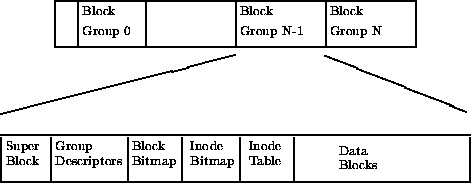
\includegraphics[height=2.5cm]{pics/img82}
  \end{center}
\end{frame}

\begin{frame}[fragile=singleslide]{Les block groups}
  \begin{itemize}
  \item  Remarque: Le bitmap  de block  doit tenir  sur un  block, par
    conséquent, il  ne peut y avoir  plus de (block\_size  * 8) blocks
    par  block group.  (aussi vrai  dans une  moindre mesure  pour les
    inodes).  C'est généralement ca  qui va déterminier la taille d'un
    groupe.
  \item  Remarque: En  connaissant,  la taille  des  block groups,  le
    nombre d'inode  par block  group et l'offset  de la  table d'inode
    dans  un group,  il est  possible d'indexer  n'importe  quel inode
    (idem pour les blocks)
  \end{itemize}
\end{frame}

\begin{frame}[fragile=singleslide]{Les inodes}
  Chaque fichier est associé à un inode. Un inode contient:
  \begin{itemize}
  \item Des  informations comme la  taille, les date  de modification,
    des création et d'accès, le type, etc...
  \item  Dans le  cas fichier  spéciaux, toutes  les  information sont
    contenus dans l'inode
  \item Un tableau  de 12 pointeur vers les  blocks contenant le corps
    du fichier (permet d'indexer les 50 premiers Ko)
  \item  Un pointeur  vers un  block contenant  des pointeurs  vers le
    corps du fichier (permet d'indexer les 4Mo suivants)
  \item un pointeur  vers un block de second  niveau (qui contient des
    pointeurs de pointeurs) (permet d'indexer les 4Go suivants)
  \item  un  pointeur vers  un  block  de  troisième niveau  (les  4To
    suivants)
    % \item  Le jours  ou ont aura  besoin d'indexer des  fichier de
    %   4Po, on ajoutera  une inférence (limite théorique de l'ordre
    %   de 10^40)
  \item Plus  le fichier est  gros, plus le nombre  d'indirections sera
    important
  \item Le système alloue en  priorité les fichiers dans le même block
    group que son inode (limite la fragmentation)
  \end{itemize}
\end{frame}

\begin{frame}[fragile=singleslide]{Les inodes}
  \begin{center}
    \includegraphics[height=6cm]{pics/Ext2-inode}
  \end{center}
  Remarque: les  premières inodes  du disque sont  réservée pour  : la
  liste des badblocks, le répertoire racine, le journal, etc...
\end{frame}

\begin{frame}[fragile=singleslide]{Les répertoires}
  \begin{columns}
    \begin{column}{4.5cm}
      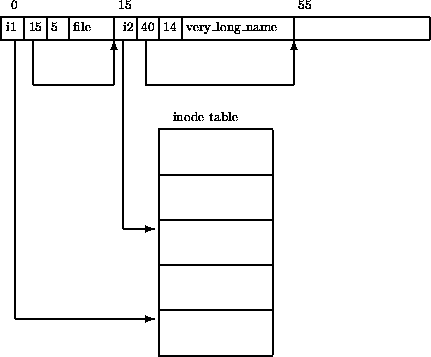
\includegraphics[height=6cm]{pics/img88}
    \end{column}
    \begin{column}{6.5cm}
      \\[3em]
      Un fichier peut-être un répertoire
      \begin{itemize}
      \item Il contient un  tableau de structures contenant l'inode du
        fichier, la taille du nom et le nom de l'entrée
      \item Un  répertoire contient systématiquement  une entrée \c{.}
        et une entrée \c{..}
      \item Une entrée dont l'inode est a zero à été supprimée
      \item Le parcours  des réperoitre se fait en  $O(n)$, un index à
        été ajouté sur ext3 pour le faire en $O(log_2(n))$
      \end{itemize}
    \end{column}
  \end{columns}

  cf.   \man{tune2fs(1)},  \man{debugfs(1)},  \man{stat(1)},
    \url{http://www.nongnu.org/ext2-doc/ext2.html}
  % Presnter le fonctionnement de fsck.ext2 (c'est interressant)
  % Exo: cacher des fichier dans de l'ext2 (il faut trouver de l'espace, ecrire, et activer la bitmap)
\end{frame}

\subsection{La journalisation}

\begin{frame}[fragile=singleslide]{Journalisation}
  \begin{itemize}
  \item Provient des technologies des bases de données
  \item Permet de garantir l'atomicité des opérations sur le disque
  \item On  écrit d'abord  dans le  journal ce que  l'on se  prépare à
    faire
  \item  Une fois  l'action écrite,  on  écrit ensuite  un message  de
    \emph{commit}
  \item Si le système plante, il  lit le journal, si une opération est
    associée à un commit, il exécute l'opération, sinon, on estime que
    les information  concernant l'opération sont  peut-être erronée et
    on exécute pas l'action
  \end{itemize}
\end{frame}

\begin{frame}[fragile=singleslide]{Journalisation}
  Evidement, il faut  de temps en temps écrire  réellement les données
  sur le disque.
  \begin{itemize}
  \item On commence par écrire les données
  \item On s'assure qu'elle ont été correctement écrite
  \item  Même si  le système  plante à  ce moment,  on  pourra rejouer
    l'entrée du journal
  \item on supprime l'entrée du journal
  \item Pour des raisons de performance, les entrée du journal ne sont
    pas forcement  écrite dans l'ordre. Il faut  alors faire attention
    aux contrainte de précédences
  \end{itemize}
  \begin{lstlisting}
$ debugfs -R logdump /dev/sda8
  \end{lstlisting}
\end{frame}

\begin{frame}[fragile=singleslide]{Journalisation}
  \begin{itemize}
  \item Il  est possible de  journaliser toutes les données  écrite ou
    seulement les meta donnée
  \item Dans le  second cas, on garanti que  filesystème sera cohérent
    mais pas les donnée à l'intérieur du fichier
  \item Linux implémente aussi  un mode \emph{ordered} qui garanti que
    les donnée sont  mise à jour sur le disque avant  de mettre à jour
    les meta  donnée. Ainsi,  il est possible  de perdre  des données,
    mais pas d'avoir des donnée corrompues.
  \end{itemize}
\end{frame}

\begin{frame}[fragile=singleslide]{Copy On Write}
  \begin{itemize}
  \item Certain file système sont dit Copy-On-Write
  \item Il sont montés read-only
  \item Si  un fichier dit  être modifié, une  copie est faite  (sur un
    autre espace ou en mémoire) et la copie est modifiée.
  \item Les futur accès ce feront sur la copie
  \item Permet de faire démarrer des  systèmes sur CD (avec un plus une
    compression dans ce cas)
  \item Permet  de faire fonctionner plusieurs système  sur une unique
    partition montée en lecture seule (virtualisation)
  \item Permet de démarrer des  machine en réseau avec un unique disque
    partagé
  \end{itemize}
\end{frame}

\section{Les RAID}

\begin{frame}[fragile=singleslide]{RAID}
  \begin{itemize}
  \item \emph{Redundant Array of Independent Disks}
  \item Peut-être matériel et transparent pour l'OS
  \item Software (cf. \man{mdadm(8)}). Le CPU doit alors s'occuper des
    différents calcul
  \item Apporte:
    \begin{itemize}
    \item Sécurité (Redondance)
    \item Performance
    \item Souplesse
    \end{itemize}
  \item  Données  regroupées en  bandes  (\emph{stripes}) de  quelques
    dizaines de kilo octets
  \item  Une  grappe  RAID est  vu  comme  un  unique disque  par  les
    filesystems de couches supérieur
  \end{itemize}
\end{frame}


\begin{frame}[fragile=singleslide]{RAID 0}
  \begin{columns}
    \begin{column}{6cm}
      \begin{itemize}
      \item Appelé \emph{Agrégation}
      \item Pas de redondance
      \item La capacité  totale est égale à la  somme des capacité des
        disques
      \item Permet de diviser les temps de lecture et écriture par $n$
      \end{itemize}
    \end{column}
    \begin{column}{4cm}
      \includegraphics[height=7cm]{pics/RAID_0}
    \end{column}
  \end{columns}
\end{frame}

\begin{frame}[fragile=singleslide]{RAID 1}
  \begin{columns}
    \begin{column}{6cm}
      \begin{itemize}
      \item Redondé $n$ fois. Permet d'avoir $n-1$ disques défaillants
      \item  La capacité  totale est  égale  la taille  du plus  petit
        disque de la grappe
      \item Pas de gain en  écriture, mais permet de diviser les temps
        d'écriture par $n$
      \end{itemize}
    \end{column}
    \begin{column}{4cm}
      \includegraphics[height=7cm]{pics/RAID_1}
    \end{column}
  \end{columns}
\end{frame}

\begin{frame}[fragile=singleslide]{RAID 2}
  \begin{itemize}
  \item Peu utilisé
  \item RAID 2: RAID 0 + ECC sur un disque séparé
  \item RAID 3: RAID 0 +  parité XOR  sur un disque séparé
    \includegraphics[height=5cm]{pics/RAID_2}
  \end{itemize}
\end{frame}

\begin{frame}[fragile=singleslide]{RAID 2}
  \begin{itemize}
  \item La parité se fait au niveau de l'octet.
  \item Les disque doivent être synchrone dans leur déplacement
  \item Les performances sont limités par le disque le plus lent
  \item Permettait de garantir la validité des données lues
  \item  ... mais,  un disque  est déjà  capable de  garantir  que les
    données sont correctes
  \item ... lors  des accès en lecture, on utilise  aussi le disque de
    parité alors que ca n'est pas utile
  \item Manque de flexibilité
  \end{itemize}
\end{frame}

\begin{frame}[fragile=singleslide]{RAID 2}
  \begin{lstlisting}
Drive #1: 00101010 (Data)
Drive #2: 10001110 (Data)
Drive #3: 11110111 (Data)
Drive #4: 10110101 (Data)
Drive #5: -------- (Hot Spare)
Drive #6: 11100110 (Parity)
  \end{lstlisting}
\end{frame}

\begin{frame}[fragile=singleslide]{RAID 2}
  \begin{lstlisting}
Drive #1: 00101010 (Data)
Drive #2:   dead   (Data)
Drive #3: 11110111 (Data)
Drive #4: 10110101 (Data)
Drive #5: -------- (Hot Spare)
Drive #6: 11100110 (Parity)
\end{lstlisting}
\end{frame}

\begin{frame}[fragile=singleslide]{RAID 2}
  \begin{lstlisting}
Drive #1: 00101010 (Data)
Drive #2:   dead   (Data)
Drive #3: 11110111 (Data)
Drive #4: 10110101 (Data)
Drive #5: 10001110 (Hot Spare)
Drive #6: 11100110 (Parity)
\end{lstlisting}
\end{frame}

\begin{frame}[fragile=singleslide]{RAID 4}
  \begin{itemize}
  \item RAID 0 + parité XOR  sur un disque séparé
  \item Ressemble au RAID 3
  \item Fonctionne par bloc plutôt que par octet
  \item Chaque disque fonctionne de manière asynchrone
  \item Permet d'optimiser les accès lecture/écriture
  \item Disymétrie  de l'usage  des disques: le  disque de  parité est
    sollicité à chaque écriture  (exemple: écritures sur les blocs A1,
    B2 et C3)
  \end{itemize}
  \begin{center}
    \includegraphics[height=4cm]{pics/RAID_4}
  \end{center}
\end{frame}

\begin{frame}[fragile=singleslide]{RAID 5}
  \begin{itemize}
  \item Evolution du RAID 4
  \item Le disque de parité n'est pas fixé
  \item Permet d'uniformiser l'usage des disques
  \end{itemize}
  \begin{center}
    \includegraphics[height=6cm]{pics/RAID_5}
  \end{center}
\end{frame}

\begin{frame}[fragile=singleslide]{RAID 6}
  \begin{itemize}
  \item Il arrive que l'opérateur change le mauvais disque
  \item  ...  ou  qu'un  second  disque  tombe  en  panne  pendant  la
    reconstruction (la loi des séries)
  \item  Remarque: Multiplier  le nombre  de disque  de parité  sur un
    RAID5 ne fonctionne pas (imaginez le cas ou deux disque de données
    tombent)
  \item L'objectif de RAID 6 est de permettre la perte de deux disques
    (ou lieu d'un seul avec le RAID 5)
  \end{itemize}
  \begin{center}
    \includegraphics[height=4cm]{pics/RAID_6}
  \end{center}
\end{frame}

\begin{frame}[fragile=singleslide]{RAID 6}
  \begin{itemize}
  \item On  utilise des codes  correcteurs de Reed-Solomon au  lieu du
    simple XOR
  \item Il est théoriquement  possible d'avoir des RAID6 permettant un
    nombre arbitraire de disque fautifs
  \item Les  implémentations actuelle  sont optimisées pour  2 disques
    fautifs
  \item Concrètement,  dans le  cas le plus  courant, on  utilise deux
    algorithmes de parités indépendants
    \begin{itemize}
    \item Le premier est un XOR classique (parité P)
    \item Le second est un XOR en appliquant tout d'abord une rotation
      de $i$ bits sur chaque octet du disque $i$ (parité Q).
    \end{itemize}
  \item Le RAID6 demande beaucoup de CPU pour calculer la parité Q. Il
    est souvent utilisé en hardware
  \end{itemize}
\end{frame}

\begin{frame}[fragile=singleslide]{RAID 6}
  Ainsi (grosso-modo, la parité Q se calcule ``en diagonale''):
  \begin{lstlisting}
Drive #1: 00101010 (Data)
Drive #2: 10001110 (Data)
Drive #3: 11110111 (Data)
Drive #4: 10110101 (Data)
Drive #5: 11100110 (Parity P)
Drive #6: 00100110 (Parity Q)
  \end{lstlisting}
\end{frame}

\begin{frame}[fragile=singleslide]{Les associations}
  \begin{itemize}
  \item Principalement utilisé pour les RAID 0 et 1
  \item A coût égal, moins performant qu'un RAID 5 ou 6
  \item  Peut néanmoins être  préférable dans  certains environnements
    techniques.
  \end{itemize}
  \begin{center}
    \includegraphics[height=5cm]{pics/RAID_01}
    \includegraphics[height=5cm]{pics/RAID_10}
  \end{center}
\end{frame}

\subsection{Un cas concret}

\begin{frame}[fragile=singleslide]{Exemple}
  Création d'un disque virtuel \c{/dev/md0}, en RAID-5 avec 3 disques:
  \begin{lstlisting}
# mdadm --create --verbose /dev/md0 --level=5 --chunk=128ko --raid-devices=3 /dev/sda1 /dev/sdb1 /dev/sdc1
# mdadm --detail /dev/md0
/dev/md0:
[...]
 Number   Major   Minor   RaidDevice State
    0       8        1        0      active sync   /dev/sda1
    1       8       17        1      active sync   /dev/sdb1
    2       8       33        2      active sync   /dev/sdc1
  \end{lstlisting}
\end{frame}

\begin{frame}[fragile=singleslide]{Exemple}
  Après un redémarrage, il faut \emph{réassembler} le RAID:
  \begin{lstlisting}
# mdadm --assemble /dev/md0 /dev/sda1 /dev/sdb1 /dev/sdc1 /dev/sdd1
  \end{lstlisting}
  ou  en scannant  les partitions  (chaque élément  du RAID  contient un
  superblock      contenant     un      identifiant      unique     de
  RAID. cf. \url{https://raid.wiki.kernel.org/index.php/RAID_superblock_formats}).
  \begin{lstlisting}
# mdadm --assemble --scan
  \end{lstlisting}
  Cette  opération  est  normalement  faite  automatiquement  par  les
  scripts de démarrage du système
\end{frame}

\begin{frame}[fragile=singleslide]{Exemple}
  Marquer un disque  défaillant (pour un test ou  parce que des erreur
  ont été détectées):
  \begin{lstlisting}
# mdadm --fail /dev/md0 /dev/sdb1
# mdadm --detail /dev/md0
/dev/md0:
[...]
Rebuild Status : 6% complete
[...]
 Number   Major   Minor   RaidDevice State
    0       8        1        0      active sync   /dev/sda1
    1       0        0        1      removed       -
    2       8       33        2      active sync   /dev/sdc1
    1       8       17        -      faulty spare  /dev/sdb1
  \end{lstlisting}
\end{frame}

\begin{frame}[fragile=singleslide]{Exemple}
  Ajout  d'un  nouveau  disque.   Le RAID  est  alors  automatiquement
  reconstruit:
  \begin{lstlisting}
# mdadm --add /dev/md0 /dev/sdd1
# mdadm --detail /dev/md0
/dev/md0:
[...]
Rebuild Status : 6% complete
[...]
 Number   Major   Minor   RaidDevice State
    0       8        1        0      active sync   /dev/sda1
    1       8       49        1      active sync   /dev/sdd1
    2       8       33        2      active sync   /dev/sdc1
    3       8       17        -      faulty spare  /dev/sdb1
  \end{lstlisting}
  Attendre la reconstruction:
  \begin{lstlisting}
# mdadm --wait /dev/md0
  \end{lstlisting}
\end{frame}

\begin{frame}[fragile=singleslide]{Exemple}
  Retirer le disque fautif:
  \begin{lstlisting}
# mdadm --remove /dev/md0 /dev/sdb1
# mdadm --detail /dev/md0
/dev/md0:
[...]
Rebuild Status : 6% complete
[...]
 Number   Major   Minor   RaidDevice State
    0       8        1        0      active sync   /dev/sda1
    1       8       49        1      active sync   /dev/sdd1
    2       8       33        2      active sync   /dev/sdc1
  \end{lstlisting}
\end{frame}

\begin{frame}[fragile=singleslide]{Exemple}
  Ajout d'un nouveau  disque de spare.  Ainsi, si  un nouveau disque a
  une défaillance,  il sera automatiquement remplacé par  le disque de
  spare:
  \begin{lstlisting}
# mdadm --add /dev/md0 /dev/sde1
# mdadm --detail /dev/md0
/dev/md0:
[...]
Rebuild Status : 6% complete
[...]
 Number   Major   Minor   RaidDevice State
    0       8        1        0      active sync   /dev/sda1
    1       8       49        1      active sync   /dev/sdd1
    2       8       33        2      active sync   /dev/sdc1
    3       8       65        -      spare         /dev/sde1
  \end{lstlisting}
\end{frame}

\begin{frame}[fragile=singleslide]{Exemple}
  Modifier le nombre de disque utilisés (pas forcement possible)
  \begin{lstlisting}
# mdadm --grow --raid-devices=4 /dev/md0
# mdadm --detail /dev/md0
/dev/md0:
[...]
Rebuild Status : 1% complete
[...]
 Number   Major   Minor   RaidDevice State
    0       8        1        0      active sync   /dev/sda1
    1       8       49        1      active sync   /dev/sdd1
    2       8       33        2      active sync   /dev/sdc1
    3       8       65        3      active sync   /dev/sde1
  \end{lstlisting}
\end{frame}
  % 4h (2h pour l'arboressence + 2h pour les algos)
  %
% This document is available under the Creative Commons Attribution-ShareAlike
% License; additional terms may apply. See
%   * http://creativecommons.org/licenses/by-sa/3.0/
%   * http://creativecommons.org/licenses/by-sa/3.0/legalcode
%
% Created: 2012-07-28 20:09:12+02:00
% Main authors:
%     - Jérôme Pouiller <jezz@sysmic.org>
%

\part{La création d'executables}

\begin{frame}
  \partpage
\end{frame}

\begin{frame}
  \tableofcontents[currentpart]
\end{frame}

%% A reformuler, revoir
\section{Compilation}

\begin{frame}[fragile=singleslide]{Compilation}
  Compilation normale:
  \begin{lstlisting}
host$ gcc -c hello.c -o hello.o
host$ gcc hello.o -o hello
host$ ./hello 1
Hello World
  \end{lstlisting} %$
\end{frame}

\subsection{Fonctionnement de la compilation}

\begin{frame}[fragile=singleslide]{Le format ELF}
  \begin{itemize}
  \item La  plupart des fichiers  manipulés par le compilateur  et les
    outils associés sont au format ELF
  \item Ce format est une série de sections et de tables
  \item  Certaines sections seront chargée en mémoires
  \item  Certaines  section  demande  à etre  simplement  allouées  en
    mémoire
  \item  \man{objdump(1)} permet  d'obtenir des  informations  que un
    fichier ELF
  \item  \man{objcopy(1)}  permet   d'extraire  des  sections  ou  de
    modifier un fichier au format ELF
  \item \man{readelf(1)}  et \man{nm(1)}, mais  \cmd{objdump} contient
    toute leurs fonctionnalités
  \end{itemize}
\end{frame}

\begin{frame}[fragile=singleslide]{La compilation}
  La compilation:
  \begin{itemize}
  \item  Execute   le  préprocesseur  (fichier   \file{.i}),  puis  le
    compilateur  vérifie la syntaxe,  le typage,  converti le  code en
    assembleur  (fichier  \file{.s})   puis  en  code  objet  (fichier
    \file{.o})
  \item L'option \file{-c} est utilisé.
  \item Le compilateur doit connaitre les signature des fonction (afin
    de vérifier correctement le typage).
  \item  Les fichiers  headers (fichiers  \file{.h})  sont nécessaires
    pour cette phase
  \item \file{-I}  permet de spécifier des  chemins supplémentaires où
    rechercher des fichiers headers (par défaut: \file{/usr/include})
  \item Si un fichier est  inclu entre double-quotes, il est recherché
    dans le même répertoire que le source.
  \item \cmd{-Wall}, \cmd{-Wextra} recommandés
  \item \cmd{-DMACRO} peut etre utilisé
  \end{itemize}
\end{frame}

\begin{frame}[fragile=singleslide]{Les symboles de debug}
  \begin{itemize}
  \item \cmd{-g}  permet d'ajouter une section  contenant des symboles
    de debug
  \item Utilisés  par les debuggueurs pour  récupérer des informations
    supplémentaire ou pour faire le lien avec les sources
  \item  Les sources  ne sont  pas  incluse dans  les informations  de
    debug.  Seul une  association entre  les adresses  du code  et les
    lignes du source est incluse.
  \item  Attention  aux  modifications   des  code  posterieurs  à  la
    compilation
  \item Cette section n'est pas chargée en mémoire.
  \item Le format utilisé s'apelle \emph{dwarf} (Debug with Arbitrary
    Record Format).
  \item \cmd{strip}  permet de retirer  les section de debug  et autre
    sections utilisé seulement les opération de link
  \end{itemize}
\end{frame}

\begin{frame}[fragile=singleslide]{Les symboles de debug}
  L'option \cmd{-g} ne change pas le code généré:
  \begin{lstlisting}
$ gcc -g -c main.c -o main-dbg.o
$ gcc -c main.c -o main-rel.o
$ ls -l
-rw-rw-r-- jpo jpo 2125 Aug 3 16:05 main-rel.o
-rw-rw-r-- jpo jpo 3720 Aug 3 16:05 main-dbg.o
$ strip *.o
$ ls -l
-rw-rw-r-- jpo jpo 2096 Aug 3 16:05 main-rel.o
-rw-rw-r-- jpo jpo 2096 Aug 3 16:05 main-dbg.o
  \end{lstlisting}
\end{frame}


\subsection{Edition de liens}

\begin{frame}[fragile=singleslide]{Inlining}
  Le compilateur peut effectuer quelques optimisations:
  \begin{itemize}
  \item Les  fonction et les  variables marquées \c{static}  ne seront
    pas exportés, et donc, pas utilisé par les autres fichier objets.
  \item  Le compilateur peut décider d'\emph{inliner} ces fonctions
  \item Si toutes les appels à une fonctions statique ont été inlinés,
    il peut supprimer la fonction du fichier objet.
  \end{itemize}
\end{frame}

\begin{frame}[fragile=singleslide]{L'édition de liens}
  \begin{itemize}
  \item  Le compilateur  ne connait  pas forcement  les  addresses des
    fonctions et des variables globale marquées \c{extern}
  \item  Les endroits  ayant  besoin de  ces fonctions/variables  sont
    remplacés par  des 0 et une  entrée est ajoutée dans  la table des
    \emph{relocation} du fichier objet (cf. \cmd{objdump -R})
  \item  On appelle  le \emph{linker}  (\c{gcc} sans  l'option \c{-c})
    pour résoudre les symboles
  \item Le linker  connait toutes les fonctions, et  toutes les tables
    de relocation.
  \item Il peut déplacer les  addresses de chargement des fonctions et
    des variables de  manière à les mettre au  plus près des fonctions
    qui  les   appellent  (optimisation  de   l'utilisation  du  cache
    d'instruction)
  \item Une  fois l'agencement des fonctions défini,  le linker résoud
    toutes les entrées des tables de relocations
  \end{itemize}
\end{frame}

\begin{frame}[fragile=singleslide]{Placement des symboles de debug}
  \begin{itemize} 
  \item Il  est possible de passer  des options au linker  à partir de
    \cmd{gcc} en utilisant \cmd{-Wl,}
  \item  Il est  possible  de placer  les  symboles de  debug dans  un
    fichier séparé.
  \item Avec l'option \cmd{--build-id=uuid}, il est possible d'ajouter
    un identifiant à la binaire
  \end{itemize} 
  \begin{lstlisting}
$ gcc -Wl,--build-id=sha1 -g main.c -o main
$ cp main -o main.dbg
$ strip --only-keep-debug main.dbg
$ strip main
$ objcopy --add-gnu-debuglink=main.dbg main
$ file main main.dbg
main:     ELF 64-bit... BuildID[sha1]=0x3adaaacf2906a5d2bfb7d415035d2e2, stripped
main.dbg: ELF 64-bit... BuildID[sha1]=0x3adaaacf2906a5d2bfb7d415035d2e2, not stripped
$ objdump -h main main.dbg
  \end{lstlisting}
\end{frame}

\begin{frame}[fragile=singleslide]{Placement des symboles de debug}
  Il est possible de livrer  la binaire à laproduction tout en gardont
  les  symboles de debug  dans un  dépôt séparé.  Il sera  possible de
  demander  au  debugueur  de  les  utiliser pour  résoudre  des  dump
  mémoire. L'identifiant  unique nous permet de garantir  que les deux
  fichiers correspondent bien. On  pourait aussi sauver le code source
  de l'application afin d'avoir toutes les informations pour debuguer.
\end{frame}

\section{Les bibliothèques}

\begin{frame}[fragile=singleslide]{Les bibliothèques}
  \begin{itemize}
  \item  Afin de  simplifier  le déploiment  des  utilitaires, il  est
    possible  d'empaqueter  un  ensemble  de fichier  objet  dans  une
    bibliothèque dite statique (fichier \file{.a}). cf. \man{ar(1)}.
  \item Dans ce cas, cela ne change rien à la procedure de link
  \item Il  est aussi possible d'utiliser  des biliothèques dynamiques
    (fichier \file{.so}). Nous y reviendrons.
  \item  Il  est  possible  de  spécifier  le  chemin  complet  de  la
    bibliothèque (dynamique ou statique)  ou de laisser le compilateur
    la trouver automatiquement avec la syntaxe \cmd{-lbrary}.  On peut
    dans ce cas lui précisier des chemins supplémentaire ou rechercher
    la bibliothèque avec \cmd{-L}
  \item  Par  défaut,  le  compilateur recherchera  les  bibliothèques
    dynamiques, sauf si l'option \cmd{-static} est utilisée
  \item  Le  linker suit  en  fait  une  des recettes  contenues  dans
    \file{/usr/lib/ldscripts/}  (en fonction  des  options passées  au
    linker).   Il   est  possible  de  fabriquer   son  propre  format
    (\cmd{ld -T}) (utile pour générer des firmwares).
  \item Voir \file{u-boot.lds}.
  \end{itemize} 
 % http://www.osdever.net/bkerndev/Docs/basickernel.htm
\end{frame}

\begin{frame}[fragile=singleslide]{Les bibliothèques}
  \begin{itemize} 
  \item  Les  symboles déclaré dans les scripts
    de link sont placé aux endroits demandé en mémoire:
    \begin{lstlisting}
void *etext;
printf("My code end at %p", &etext);
    \end{lstlisting} 
  \item \cmd{-Map=file} permet de sauver le mapping mémoire utilisé
    \begin{lstlisting}
$ gcc -g -Wl,-Map=main.map main.c -o main
    \end{lstlisting} 
  \end{itemize}
\end{frame}

\begin{frame}[fragile=singleslide]{Libtool}
  Problème:
  \begin{itemize}
  \item Les  fichiers objets des bibliothèques  statiques et dynamique
    ne  se  compilent  pas  avec  les mêmes  options  (en  particulier
    \cmd{-fPIC})
  \item  Certaines architectures ne  permettent pas  les bibliothèques
    dynamiques
  \item La  création de bibliothèques  portables peut devenir  un vrai
    casse tête
  \end{itemize}
  \emph{libtool} est outil permettant de faciliter ce travail.
\end{frame}

\subsection{Les bibliothèques dynamiques}

\begin{frame}[fragile=singleslide]{Les bibliothèques dynamiques}
  L'usage de bibliothèques dynamique permet:
  \begin{itemize}
  \item de ne charger qu'un exemplaire de la bibliothèque pour tout le
    système
  \item de simplifier la redistribution du programme
  \item de simplifier les mises à jour de la bibliothèque
  \end{itemize}
\end{frame}

\begin{frame}[fragile=singleslide]{Les bibliothèques dynamiques}
  Coté bibliothèque:
  \begin{itemize}
  \item  Elle contient  une table  des  symboles exportés  et de  leur
    emplacement (dans la table \emph{.dynsym})
  \item A  la construction, elle  doit être linkée  avec \cmd{-shared}
    pour indiquer  que sont  chargement sera différent  d'un programme
    standard (principalement, aucune fonction main n'est nécessaire)
  \end{itemize}
\end{frame}

\begin{frame}[fragile=singleslide]{Les bibliothèques dynamiques}
  Coté éxecutable:
  \begin{itemize}
  \item Le  linker va ajouter une table  d'indirection (la \emph{.got}
    \emph{Global  Offset Table})  pour tous  les symboles  se trouvant
    dans des bibliothèques
  \item Le linker doit passer  par cette indirection pour appeller une
    fonction exportée par une biliothèque dynamique.
  \item Il ne peut pas faire  tenir ce morceau de code à l'emplacement
    laissé par le compilateur (qui  ne fait pas la différence entre un
    symbole statique et un symbole dynamique)
  \item Il crée  donc un petit morceau de code  qu'il placera dans une
    section \emph{Procedure Linkage Table} (\emph{.plt})
  \item Cette  procedure permet simplement  de brancher vers  la table
    d'indirection.
  \end{itemize}
\end{frame}

\begin{frame}[fragile=singleslide]{Les bibliothèques dynamiques}
  \begin{center}
   \pgfimage[width=7cm]{pics/plt_after}
\end{center}
\begin{lstlisting}
$ objdump -d | grep -A 10 "section \.plt"
    \end{lstlisting}
\end{frame}

\begin{frame}[fragile=singleslide]{Les bibliothèques dynamiques}
  A l'éxécution
  \begin{itemize}
  \item Un interpreteur (normalement \file{/lib/ld.so}) est appellé
  \item  Il charge  les bibliothèques  nécessaires (inscrites  dans la
    table \emph{.dynamic}) en mémoire
  \item  Il  remplit la  GOT  avec  des  pointeurs vers  une  fonction
    permettant la résolution du symbole.
  \item Lorsque ce symbol est appellé la première fois, cette fonction
    est appellée.
  \item La fonction résoud le symbol et place son adresse dans la GOT
  \item Cette méthode s'appelle \emph{lazy resolving}
  \item   Cela   peut   être   désactivé  en   passant   la   variable
    d'environnement \cmd{LD_BIND_NOW}
  \end{itemize}
\end{frame}

\begin{frame}[fragile=singleslide]{Les bibliothèques dynamiques}
  \begin{center}
    \pgfimage[width=7cm]{pics/plt_before}
  \end{center}
\end{frame}

\begin{frame}[fragile=singleslide]{Les bibliothèques dynamiques}
  \begin{itemize}
  \item Il est possible de  demander le chargement manuel et dynamique
    des    bibliothèques    et    des    symboles    avec    \c{libdl}
    (\man{dl\_open(3)}, \man{dl\_sym(3)})
  \item Afin d'accélérer le  chargement, \file{ld.so} utilise un index
    de bibliothèques présentes sur le système.
  \item  Lorsque vous  ajoutez une  bibliothèque, vous  devez appeller
    \man{ldconfig(1)} pour mettre à jour ce cache.
  \item la  variable \cmd{LD_LIBRARY_PATH} permet  d'ajouter un chemin
    de recherche de biliothèque pour \file{ld.so}.
  \end{itemize}
\end{frame}

\begin{frame}[fragile=singleslide]{Utilisation de \c{LD_PRELOAD}}
  \begin{itemize}
  \item La  variable d'envionnement \c{LD_PRELOAD}  permet de demander
    le chargement d'une bibliothèque avant les autres
  \item Les symboles exportées par celle-ci seront prioritaires.
  \item Exemple:
    \begin{lstlisting}
unsigned int sleep(unsigned int s) {
    static unsigned int (*real_sleep)(unsigned int s) = NULL;

    if (!real_sleep)
        real_sleep = dlsym(RTLD_NEXT, ``sleep'');

    usleep(5);
    return real_sleep(s);
}
    \end{lstlisting}
  \end{itemize}
\end{frame}

\section{Résultats de la compilation}
% Section: Redistribution? A deplacer apres les outils de compilation?

\begin{frame}[fragile=singleslide]{A qui fournir quoi?}
  \begin{itemize}
  \item La poubelle
    \begin{itemize}
    \item Les dependances
    \item Les objets (ELF)
    \end{itemize}
  \item Les sources
    \begin{itemize}
    \item Les sources
    \item Les headers
    \item Le système de compilation
    \end{itemize}
  \item Les developpeurs externes
    \begin{itemize}
    \item Les headers
    \item Les bibliothèque statique (archve crée avec \man{ar(2)})
    \end{itemize}
  \item L'utilisateur final
    \begin{itemize}
    \item Les bibliothèque dynamique (ELF)
    \item Les binaires (ELF)
    \end{itemize}
  \end{itemize}
\end{frame}

\begin{frame}[fragile=singleslide]{Identifier le résultat}
  Un bon moyen de reconnaitre  les binaires est d'utiliser la commande
  \man{file(1)}:
  \begin{lstlisting}
host$ file ...
hello-dyn:        ELF 64-bit LSB executable, x86-64, version 1 (SYSV), dynamically linked (uses shared libs), for GNU/Linux 2.6.15, not stripped
hello-static: ELF 64-bit LSB executable, x86-64, version 1 (GNU/Linux), statically linked, for GNU/Linux 2.6.15, not stripped
/lib/x86_64-linux-gnu/librt-2.15.so: ELF 64-bit LSB shared object, x86-64, version 1 (SYSV), dynamically linked (uses shared libs), for GNU/Linux 2.6.24, stripped
/usr/lib/x86_64-linux-gnu/librt.a: current ar archive
\end{lstlisting} %$
\end{frame}

\begin{frame}[fragile=singleslide]{Redistribution et licences}
  \begin{itemize}
  \item GPL. Est-ce du travail dérivé?
    \begin{itemize}
    \item Le resultat d'un copier-coller?
    \item Une compilation statique?
    \item Une compilation dynamique?
    \end{itemize}
  \item LGPL
  \end{itemize}
\end{frame}

\section{Makefiles}
% A étoffer?

\begin{frame}[fragile=singleslide]{Makefile}
  \begin{itemize} 
  \item Vieux système (qui a dit ``pourri''?)
  \item Beaucoup d'implémentations différentes
  \item Heureusement,  gmake (GNU Make) est quasiment  le seul utilisé
    de nos jours.
  \item  \cmd{make}  est finalement  un  interpréteur  qui éxecute  le
    fichier  nommé  \file{Makefile}  ce  trouvant dans  le  répertoire
    courant
  \item  Il existe  de nombreuses  alternatives au  Makefile,  mais ce
    dernier  a imposé des  standards qui  se retrouvent  dans beaucoup
    d'autres systèmes (nous en verrons quelques uns plus tard)
  \end{itemize} 
\end{frame} 

\begin{frame}[fragile=singleslide]{Bases}
  \begin{itemize} 
  \item Principe du fichier \file{Makefile}:
    \begin{lstlisting} 
cible: depends
       rules
file.o: file.c dep.h
       gcc file.c -c -o file.o
    \end{lstlisting} 
  \item \cmd{make} crée  un graphe de dépendance et  vérifie les dates
    de modifications  des fichierx afin  de n'éxecuter que  les règles
    nécessaires
  \item Notez que les  dépendances avec les fichiers \file{.h} doivent
    être déclarées
  \item Un \file{Makefile} bien écrit ne reconstruit que le nécessaire
    et n'oublie jamais de reconstruire le nécessaire.
  \item  Il  est  possible  spécifier  à  make une  ou  des  cibles  à
    fabriquer. Sinon, il fabriquera la première cible seulement.
  \end{itemize}
\end{frame}

\begin{frame}[fragile=singleslide]{Les variables}
  \begin{itemize} 
  \item Il est possible d'utiliser des variables
    \begin{lstlisting}
CC = gcc
...
        $(CC) file.c -c -o file.o
    \end{lstlisting} %$
  \item Remarquez que la syntaxe des variable est différente du shell.
  \item ... or, nous appellons du shell à partir des \file{Makefile}
  \item  Les  variables  peuvent  être  surchargées sur  la  ligne  de
    commande:
    \begin{lstlisting}
$ make CC=special-gcc
    \end{lstlisting} %$
  \item  Il  existe de  nombreuses  variables standards,  prédéfinies:
    \c{CC}, \c{CFLAGS},  \c{LDFLAGS}, \c{CXX}, \c{CXXFLAGS}, \c{MAKE},
    ...
  \item  Il existe  aussi des  variables locales  aux  règles: \c{$<},
    \c{$@}, ....
  \end{itemize} 
\end{frame}

\begin{frame}[fragile=singleslide]{Makefile}
  \begin{itemize} 
  \item  Il  est  possible  de définir  des  règles
    génériques:
    \begin{lstlisting} 
%.o: %.c
       gcc $< -c -o $@
file.o: dep.h
    \end{lstlisting} 
  \item De plus, il existe de nombreuses règles implicite qui facilite
    le travail
  \item  Utilisez  au maximum  les  règles  implicites facilite  votre
    travail:
    \begin{lstlisting}
host$ vi toto.c
host$ touch Makefile
host$ make toto
    \end{lstlisting} %$
    \item Un bon Makefile est un Makefile court
  \end{itemize}
\end{frame}

\begin{frame}[fragile=singleslide]{Les règles \emph{phony}}
  \begin{itemize} 
  \item  Il  est  possible  de définir  des  règles  \emph{virtuelles}
    (\emph{phony}) pour simplifier certains traitements
    \begin{lstlisting}
all: exec1 exec2
    \end{lstlisting} 
  \item  Parmis  les règles  \emph{phony}  très répandues:  \c{clean},
    \c{distclean},   \c{install},    \c{all},   \c{check},   \c{dist},
    \c{distcheck}, \c{mrproper}...
  \end{itemize} 
\end{frame}
 % 2h
  %
% This document is available under the Creative Commons Attribution-ShareAlike
% License; additional terms may apply. See
%   * http://creativecommons.org/licenses/by-sa/3.0/
%   * http://creativecommons.org/licenses/by-sa/3.0/legalcode
%
% Created: 2012-07-28 20:09:12+02:00
% Main authors:
%     - Jérôme Pouiller <jezz@sysmic.org>
%

\part{Systèmes de compilation}

{
\setbeamertemplate{background canvas}{}
\begin{frame}[plain]
  \partpage
  \begin{textblock}{10}(6,12)
    \begin{quote}
      \rmfamily\textit\textbf\color{darkgray}{\large
      ``Real Programmers don't comment their code. If it was hard to write, it should be hard to understand.''}
      %\vskip3mm\hspace*\fill{\small--- William Shakespeare, Hamlet}
    \end{quote}
  \end{textblock}
\end{frame}
}

\begin{frame}
  \tableofcontents
\end{frame}

% (Re-ajouter l'utilisation des systeme de compilations)


% A placer au debut de la section compilation
\begin{frame}[fragile=singleslide]{Règle d'or}
  \begin{center}
    \huge{Jamais d'espaces dans les chemins de compilation}
  \end{center}
\end{frame}

\subsection{Un projet base de Makefile}

\begin{frame}[fragile=singleslide]{Qu'est-ce qu'un cross-compiler?}
  \begin{itemize}
  \item Permet de compiler vers une cible différente du host
  \item Les binaires produites ne sont pas éxecutable sur le host
  \item La cible de la compilation est généralement décrites dans le nom
  \end{itemize}
  \begin{lstlisting}
$ /opt/arm-sysmic-linux-uclibcgnueabi/usr/bin/arm-buildroot-linux-uclibcgnueabi-gcc source.c
$ PATH+=:/opt/arm-sysmic-linux-uclibcgnueabi/usr/bin/
$ arm-buildroot-linux-uclibcgnueabi-gcc source.c
$ file a.out
a.out: ELF 32-bit LSB executable, ARM, version 1 (SYSV), dynamically linked (uses shared libs), not stripped
  \end{lstlisting}
\end{frame}

\begin{frame}[fragile=singleslide]{Cas générique}
  On utilise les variables prédéfinies de gmake:
  \begin{lstlisting}
make CC=arm-linux-gcc
  \end{lstlisting}
  Mieux dans un sous répertoire séparé:
  \begin{lstlisting}
mkdir arm
cd arm
make -f ../Makefile VPATH=.. CC=arm-linux-gcc
  \end{lstlisting}
  Exemple avec memstat.
\end{frame}

\begin{frame}[fragile=singleslide]{Créer un projet sans autotools}
  Utiliser au maximum les règles implicites facilite votre travail
  \begin{lstlisting}
host$ touch Makefile
host$ make hello
  \end{lstlisting} %$
\end{frame}

\begin{frame}[fragile=singleslide]{Créer un projet sans autotools}
  Utiliser les règles implicites facilite votre travail
  \lstinputlisting{samples/hello/Makefile.1}
  Testons:
\begin{lstlisting}
host$ make CC=arm-linux-gcc CFLAGS=-Wall
\end{lstlisting} %$
\end{frame}

\begin{frame}[fragile=singleslide]{Créer un projet sans autotools}
  \cmd{VPATH} vous permet de géré la compilation \emph{out-of-source}.
  Remarques que pour que \verb+VPATH+ fonctionne correctement, vous devez avoir
  correctement utilisé le quoting pour les directive d'inclusion (\verb+<+ pour
  les entête systèmes et \verb+"+ pour les entêtes du projet)
  % Pas besoin d'ajouter VPATH = . Du coup, c'est la meme chose que Makefile.1
  %\lstinputlisting{samples/hello/Makefile.2}
  Testons:
\begin{lstlisting}
host$ cd build
host$ make -f ../Makefile VPATH=.. CC=arm-linux-gcc
\end{lstlisting} %$
\end{frame}

\begin{frame}[fragile=singleslide]{Créer un projet sans autotools}
  \cmd{gcc} peut  générer les dépendances de vos  fichiers.  On génère
  ainsi  des morceaux  de Makefile  que l'on  inclut. Il  ne  faut pas
  oublier   d'ajouter  la  dépendance   entre  \cmd{hello.d}   et  les
  dépendances de \cmd{hello.c}
  \lstinputlisting{samples/hello/Makefile.3}
  \note{ Voir http://www.makelinux.net/make3/make3-CHP-2-SECT-7.html}
\end{frame}

\begin{frame}[fragile=singleslide]{Créer un projet sans autotools}
  Les  Makefile permettent d'utiliser  des fonctions  de substitutions
  qui  peuvent  nous aider  à  rendre  notre  système plus  générique.
  \lstinputlisting{samples/hello/Makefile.4}
\end{frame}

\begin{frame}[fragile=singleslide]{Créer un projet sans autotools}
  Nous pouvons  ajouter des alias  pour nous aider dans  les commandes
  complexes
  \lstinputlisting[firstline=10]{samples/hello/Makefile.5}
  \note[item]{TODO: Ajouter des \#ifdef CONFIG pour faire dans Kconfig}
  \note[item]{Parler de apt-get source (-b), dpkg -L, dpkg -l, dpkg-buildpackage}
\end{frame}

\subsection{A base d'Autotools}

\begin{frame}[fragile=singleslide]{Historique des Autotools}
  \note[item]{Faire l'historique de configure/Makefile/autotools}
  \begin{enumerate}
  \item Makefile
  \item Makefile + hacks pour effectuer de la configuration
  \item Makefile.in + configure
  \item Makefile.in + configure.ac
  \item Makefile.am + configure.ac
  \end{enumerate}
\end{frame}

\begin{frame}[fragile=singleslide]{Compiler avec autotools}
  \begin{itemize}
  \item C'est le cas le plus courant
  \item Pour une compilation classique:
\begin{lstlisting}
host$ ./configure
host$ make
host% make install
\end{lstlisting} %$
  \item Exemple avec dropbear.
  \item Compilation \emph{out-of-source}. il est nécessaire d'appeller
    le \file{configure} à partir du répertoire de build.
    \begin{lstlisting}
host$ mkdir build
host$ cd build
host$ ../configure
host$ make
host% make install
    \end{lstlisting} %$
  \end{itemize}
\end{frame}

\begin{frame}[fragile=singleslide]{Compiler avec autotools}
  Obtenir de l'aide:
\begin{lstlisting}
host$ ./configure --help
\end{lstlisting} %$

  Parmis les fichiers générés:
  \begin{itemize}
  \item \file{config.log}  contient la sortie  des opération effectuée
    lors de l'appel de \cmd{./configure}.  En particulier, il contient
    la ligne de commande utilisée. Il est ainsi possible de facilement
    dupliquer la configuration.
\begin{lstlisting}
host$ head config.log
\end{lstlisting} %$
  \item     \cmd{config.status}     permet     de    regénérer     les
    Makefile.  \cmd{config.status} est  automatiquement appellé  si un
    Makefile.am est modifié.
  \end{itemize}
  \note{Ajouter un exemple avec tcpdump ou dmalloc}
\end{frame}


\begin{frame}[fragile=singleslide]{Créer un projet avec autotools}
  Fonctionnement des autotools:
  \begin{itemize}
  \item Préparation
\begin{lstlisting}
% apt-get install automake autoconf
\end{lstlisting}
  \item Déclaration de notre programme et de nos sources pour \cmd{automake}
\begin{lstlisting}
$ vim Makefile.am
\end{lstlisting} %$
\begin{lstlisting}
bin_PROGRAMS = hello
hello_SOURCES = hello.c hello.h
\end{lstlisting}
%  \item Les \cmd{autotools}  imposent l'existence de certains fichiers
%    de documentation
%\begin{lstlisting}
%$ touch NEWS README AUTHORS ChangeLog
%\end{lstlisting} %$
  \end{itemize}
\end{frame}

\begin{frame}[fragile=singleslide]{Créer un projet avec autotools}
  \begin{itemize}
  \item  Création  d'un  template  pour \cmd{autoconf}  contenant  les
    macros utiles pour notre projet
\begin{lstlisting}
$ autoscan
$ mv configure.scan configure.ac
$ rm autoscan.log
$ vim configure.ac
\end{lstlisting}
  \item Personnalisation du résultat
\begin{lstlisting}
...
AC_INIT([hello], [1.0], [bug@sysmic.org])
AM_INIT_AUTOMAKE([foreign])
...
\end{lstlisting}
  \item      Génération      du      \file{configure}      et      des
    \file{Makefile.in}. C'est cette version qui devrait être livée aux
    packageurs.
\begin{lstlisting}
$ autoreconf -iv
\end{lstlisting} %$
    \note[item]{Bon, pas de TP la dessus, ca pas très utile}
  \end{itemize}
\end{frame}

\begin{frame}[fragile=singleslide]{Créer un projet avec autotools}
  \begin{itemize}
  \item Compilation
\begin{lstlisting}
$ ./configure --help
$ mkdir build
$ cd build
$ ../configure --host=arm-linux --build=i386 --prefix=$(pwd)/../install
$ make
$ make install
\end{lstlisting} %$
  \end{itemize}
\end{frame}

\begin{frame}[fragile=singleslide]{Créer un projet avec autotools}
  La cible \verb+distcheck+ :
  \begin{enumerate}
  \item Recopie les fichiers référencé dans Autotools
  \item Retire les droits en écriture sur les sources
  \item Lance une compilation \emph{out-of-source}
  \item Installe le projet
  \item Lance la suite de test
  \item Lance un distclean
  \item Vérifie que tous les fichiers créés sont effectivement supprimés
  \item Crée une tarball correctement nommée contenant les sources
  \end{enumerate}
\end{frame}

\begin{frame}[fragile=singleslide]{Créer un projet avec autotools}
  Si \cmd{automake}  est appellé avec  \verb+-gnits+, \verb+distcheck+
  effectue des vérification supplémentaires sur la documentation,
  etc...
  \\[2ex]
  La fonctionnalité \verb+distcheck+ est  le point fort souvent énoncé
  des autotools.
\begin{lstlisting}
$ make distcheck
$ tar tvzf hello-1.0.tar.gz
\end{lstlisting} %$
\end{frame}

%%% A partir de la, je ne sais pas si je le fais

\subsection{A base kmake}

%% A placer apres le système de Makefile?
%% Peut-être ajouter léxemple d'eolane juste avant
\begin{frame}[fragile=singleslide]{Compiler un programme tiers}{Kconfig}
  \begin{itemize}
  \item Système de compilation du noyau
  \item Très bien adapté à la cross-compilation
  \item Pour configurer les options:
    \begin{itemize}
    \item En ncurses
\begin{lstlisting}
host% apt-get install libncurses5-dev
host$ make ARCH=arm CROSS_COMPILE=arm-linux- menuconfig
\end{lstlisting} %$
    \item En Qt3
\begin{lstlisting}
host% apt-get install libqt3-mt-dev
host$ make ARCH=arm CROSS_COMPILE=arm-linux- xconfig
\end{lstlisting} %$
    \end{itemize}
  \item Ne pas oublier d'installer les headers des bibliothèques
    \item Exemple avec busybox
  \end{itemize}
\end{frame}

\begin{frame}[fragile=singleslide]{Compiler un programme tiers}{Kconfig}
  \begin{itemize}
  \item Pour cross-compiler
\begin{lstlisting}
host$ make ARCH=arm CROSS_COMPILE=arm-linux-
\end{lstlisting} %$
  \item Pour compiler \emph{out-of-source}
\begin{lstlisting}
host$ mkdir build
host$ make ARCH=arm CROSS_COMPILE=arm-linux- O=build
\end{lstlisting} %$
  \end{itemize}
\end{frame}

\begin{frame}[fragile=singleslide]{Compiler un programme tiers}{Kconfig}
  Principaux points importants:
  \begin{itemize}
  \item Adapté au environnements embarqué
  \item Adapté aux environnements avec beaucoup de configuration
  \item Initié par le Kernel Linux
  \item  Pas un  système de  compilation réel. Composé de :
    \begin{itemize}
    \item Kconfig, Système de gestion de configuration
    \item  Kmake, règles  Makefile  bien étudiées.  Chaque projet  les
      adapte à ces besoins
    \end{itemize}
  \item Application de la règle: "Pas générique mais simple à hacker"
  \item Dépend principalement de \cmd{gmake}
  \item Mode verbose: \verb+V=1+
  \item Permet d'effectuer des recherche
  \end{itemize}
\end{frame}

\begin{frame}[fragile=singleslide]{Compiler un programme tiers}{Kconfig}
  Test avec busybox:
  \begin{itemize}
  \item Préparation
\begin{lstlisting}
host$ wget http://busybox.net/downloads/busybox-1.18.3.tar.bz2
host$ tar xvjf busybox-1.18.3.tar.bz2
\end{lstlisting} %$
  \item Récupération d'une configuration par défaut
\begin{lstlisting}
host$ make help
host$ make ARCH=arm CROSS_COMPILE=arm-linux- O=build defconfig
\end{lstlisting} %$
  \item Personnalisation de la configuration
\begin{lstlisting}
host% apt-get install libncurses5-dev
host$ make ARCH=arm CROSS_COMPILE=arm-linux- O=build menuconfig
\end{lstlisting} %$
  \end{itemize}
\end{frame}

\begin{frame}[fragile=singleslide]{Compiler un programme tiers}{Kconfig}
  Test avec busybox:
  \begin{itemize}
  \item Compilation
\begin{lstlisting}
host$ make ARCH=arm CROSS_COMPILE=arm-linux-
\end{lstlisting} %$
  \item Installation
\begin{lstlisting}
host$ make ARCH=arm CROSS_COMPILE=arm-linux- install
\end{lstlisting} %$
  \end{itemize}
\end{frame}

\subsection{A base de Cmake}

\begin{frame}[fragile=singleslide]{Cmake}
  \begin{itemize}
  \item Aucune des  solution précédentes ne fonctionne sur  les OS non
    posix (rappel: Cygwin = Couche posix pour Windows)
  \item Cmake ressemble à Automake + Autoconf
  \item Un fichier (CMakeLists.txt) décrit la compilation
    \begin{lstlisting}
cmake_minimum_required (VERSION 2.6)
project (HELLO)
add_executable (hello hello.c)
    \end{lstlisting}
  \item Exemple avec yajl
  \item Cmake génère des fichiers  pour les différent types de système
    de compilation: Makefile, XCode, projet VisualStudio, etc...
    \begin{lstlisting}
$ mkdir build
$ cd build
$ ccmake ..
$ make
    \end{lstlisting}
\end{itemize}
\end{frame}

\begin{frame}[fragile=singleslide]{Cmake}
  Points positifs:
  \begin{itemize}
  \item Portabilité
  \item Syntaxe cohérente (c'est loin d'être le cas de Makefile)
  \item Extensible
  \item  Son  abstration permet  une  prise  en  main facile  pour  un
    débutant
  \end{itemize}
  Sa portabilité rend le niveau d'abstraction de Cmake assez élevé:
  \begin{itemize}
  \item Peut dérouter les habitués
  \item Processus de compilation  complexe à debugguer (c'est aussi le
    cas d'Autotools)
  \item  Faible intégration  avec  les système  de compilation  natifs
    (contrairement à Autotools)
  \item  Certaine action  simple nativement  peuvent  devenir complexe
    dans Cmake
  \item  Nécessite d'installer  cmake  sur la  machine de  compilation
    (Contrairement à Autotools/Kmake)
  \end{itemize}
\end{frame}

\begin{frame}[fragile=singleslide]{Que choisir?}
  \begin{itemize}
  \item  Projet nécessitant  une  bonne integration  avec les  système
    Posix et avec les système Microsoft: Cmake
  \item  Petit  projet, avec  redistribution  restreinte: Makefile  ou
    CMake
  \item Petit projet, mais redistribution large: Autotools
  \item Gros projet de forte complexité: Kmake
  \end{itemize}
\end{frame}
 %2h
  %%
% This document is available under the Creative Commons Attribution-ShareAlike
% License; additional terms may apply. See
%   * http://creativecommons.org/licenses/by-sa/3.0/
%   * http://creativecommons.org/licenses/by-sa/3.0/legalcode
%
% Created: 2011-08-14 17:43:38+02:00
% Main authors:
%     - Jérôme Pouiller <jezz@sysmic.org>
%

\part{Fonctionnement monotâches}

\begin{frame}
  \partpage
\end{frame}

\begin{frame}
  \tableofcontents[currentpart]
\end{frame}

\begin{frame}{Les OS monotâches}
  \begin{itemize}
  \item Permettent  surtout de fournir une  interface de programmation
    commune pour différents programmes ou drivers
  \item Le plus connu est sûrement MS-DOS
  \item Les OS génériques sont maintenant tous multitâches
  \item  Les  derniers  restant   se  trouvent  sur  des  applications
    spécialisés : Consoles de jeux, calculatrice, etc...
  \item Ils ont l'intérêt d'être simple à développer
  \end{itemize}
\end{frame}

\begin{frame}{Une définition}
  \begin{itemize}
  \item \textbf{Temps de réponse} : temps entre un évènement et la fin
    du traitement de l'évènement.
  \end{itemize}
\end{frame}

\section{Scrutation des évènements}
\begin{frame}[fragile]{Scrutation des évènements}
  \begin{itemize}
  \item Aussi appelé \emph{polling}
  \item Boucle infinie
  \item On teste des valeurs des entrées à chaque tour de boucle
  \end{itemize}
  \begin{lstlisting}
#define sensor1 *((char *) 0x1234)
#define sensor2 *((char *) 0xABCD)

int main() {
  while (1) {
    if (sensor1)
      action1();
    if (sensor2)
      action2();
  }
}
  \end{lstlisting}
\end{frame}

\begin{frame}{Scrutation}
  \begin{itemize}
  \item Temps de réponse au  évènements en pire cas facile à calculer:
    Pire temps pour parcourir la boucle
  \item Simple à programmer lorsqu'il  y a peu de périphériques (ayant
    des temps  de réaction  similaires). On peut  les scruter  en même
    temps
  \item Utilisation du CPU sous optimal. Beaucoup de temps est utilisé
    pour lire la valeur des  entrée. Ceci est particulièrement vrai si
    les évènements sont peu fréquents
  \item Si certains évènements entraînent des temps de traitement long
    ou si il y a beaucoup  d'entrées à scruter, le temps de réponse en
    pire cas peut rapidement devenir très grand
  \item Tous les évènements sont traités avec la même priorité
  \item  Mauvaise modularité  du code.  Ajouter des périphériques
    revient à repenser tout le système
  \end{itemize}
\end{frame}

\section{Gestion d'interruptions synchrones}

\begin{frame}{Interruptions synchrones}
  \begin{itemize}
  \item Appelé aussi Background/Foreground
  \item Gestion des évènements dans les interruptions
  \end{itemize}
  \begin{center}
    \pgfimage[width=6cm]{pics/model_bgfg}
  \end{center}
\end{frame}

\begin{frame}[fragile]{Interruptions synchrones}
  Concrètement:
  \begin{lstlisting}
#define PTR_DATA ((char *) 0x1234)

void isr() {
  action1(*PTR_DATA);
  *PTR_DEVICE_ACK = 1;
}

int main() {
  enable_interrupt(isr, 0x1);
  while(1) {
    ; // Optionnal background computing
  }
}
  \end{lstlisting}
\end{frame}

\begin{frame}{Interruptions synchrones}
  \begin{itemize}
  \item Temps de réponse au évènements plutôt bon
  \item Temps de réponse assez simple à calculer. Somme de
    \begin{itemize}
    \item Temps de traitement de l'évènement
    \item Temps de traitement des évènements de priorité supérieures
    \item Temps du changement de contexte (plus ou moins constant)
    \item Pire intervalle de temps ou les interruptions sont désactivées
    \end{itemize}
  \item[$\rightarrow$] Dans  un système simple, ça peut  se calculer à
    la louche
  \item Le  temps de réponse en pire  cas des calculs en  tâche de fond
    est quasiment  identique au traitement  par scrutation (attention
    tout de même à la fréquence maximum des interruptions)
  \end{itemize}
\end{frame}

\begin{frame}{Qu'est-ce qu'une interruption?}
  Il existe trois type d'interruptions:
  \begin{itemize}
  \item Les interruptions matérielles:
    \begin{itemize}
    \item   \textbf{IRQ}   (aussi   appelé   Interruption   externe).
      Asynchrone.   Exemples:  clavier,   horloge,  bus,  DMA,  second
      processeur, etc...
    \item  \textbf{Exception}.   Asynchrone  ou Synchrone.   Exemples:
      Division  par zéro,  Erreur arithmétique,  Erreur d'instruction,
      Erreur d'alignement, Erreur de page, Breakpoint matériel, Double
      faute,  etc...

      \note{Un  overflow arithmétique ne  produit pas  d'exception, il
        lève le flags ``retenue''\\}

      \note{Un  breakpoint  logiciel change  une  instruction par  une
        interruption  logicielle. Un  break point  software  n'est pas
        possible en ROM alors que le breakpoint hardware oui\\}
    \end{itemize}
  \item \textbf{Logicielle}. Déclenchée par une instruction. Synchrone.
  \end{itemize}
\end{frame}

\begin{frame}{Fonctionnement d'une interruption}
  \begin{center}
    \pgfimage[width=10cm]{pics/interuption-1}
  \end{center}
\end{frame}

\begin{frame}{Fonctionnement d'une interruption}
  Quand une  interruption est levée:
  \begin{itemize}
  \item le CPU sauve en  partie ou en totalité le contexte d'exécution
    (principalement le pointeur d'instruction) sur la pile
  \item Le CPU passe en mode superviseur (nous y reviendrons)
  \item  Le CPU  recherche dans  l'IVT (\emph{Interrupt  Vector Table}
    aussi  appelée  IDT,  \emph{Interrupt  Description  Table})  l'ISR
    (\emph{Interruption Service Routine}) associée
  \item Le CPU place le pointeur d'instruction sur l'ISR
  \item  L'ISR traite  l'évènement (fin  de traitement  d'une E/S,
    etc...)
  \item L'ISR acquitte la  réception de l'interruption indiquant qu'une
    nouvelle  donnée peut-être  traitée.
  \item L'ISR restaure le (un) contexte
  \end{itemize}
\end{frame}

\begin{frame}{Fonctionnement d'un PIC}
  Le PIC (Programmable Interrupt Controller) est un composant matériel
  permettant  la gestion  des  IRQ.  Il peut-être  intégré  au CPU  ou
  externe (ou à cheval entre les deux...). Il permet en particulier:
  \begin{itemize}
  \item Activer ou de désactiver des IRQ
  \item De masquer temporairement une IRQ
  \item De mettre en queue une interruption temporairement masquée
  \item De contrôler la priorité des interruptions
  \end{itemize}
  Il arrive fréquemment  qu'un PIC soit multiplexé sur  une seule ligne
  d'IRQ. Dans  ce cas, le premier  étage d'ISR lit un  registre du PIC
  pour connaître  le numéro de l'IRQ.   (Cas notoire du  8259A sur les
  architectures x86)

  \note {Il existe aussi des APIC (Advanced PIC). Sur PC notamment}
\end{frame}

\begin{frame}{Exemple}
  Exemple classique d'intégration d'un PIC multiplexé sur une IRQ:
  \begin{center}
    \pgfimage[width=10cm]{pics/interuption-3}
  \end{center}
\end{frame}

\begin{frame}{Exemple}
  \begin{enumerate}
  \item Le périphérique \emph{Timer} lève sa ligne d'IRQ
  \item Le PIC reçoit l'interruption et lève une IRQ du processeur
  \item  Le processeur  complète  l'instruction courante  et sauve  le
    registre d'instruction (PC) et le registre d'état (PSW)
  \item La tâche courante devient interrompue (Nous y reviendrons)
  \item Le premier étage d'ISR est appelé
  \item  Le  gestionnaire d'interruption  complète  la sauvegarde  des
    registres
  \item   Le  gestionnaire  d'interruption   demande  au   PIC  quelle
    interruption à  été appelée  et il lit  dans l'IVT quelle  ISR est
    associée
  \end{enumerate}
\end{frame}

\begin{frame}{Exemple}
  \begin{enumerate}
    \setcounter{enumi}{7}
  \item Le  gestionnaire d'interruption se branche  sur l'ISR associée
    (ici, ISR1)
  \item L'IRQ du processeur est acquittée. Les autre IRQ peuvent ainsi
    être levées
  \item  L'ISR1 lit la  valeur provenant  du \emph{Timer}  et acquitte
    l'interruption  du \emph{Timer}. Ce  périphérique peut  de nouveau
    lever des IRQ.
  \item Les registres généraux sont restaurés
  \item Le contexte d'exécution est restauré
  \item Le registre PC est restauré
  \end{enumerate}
\end{frame}

\subsection{Utilisation des interruptions}

\begin{frame}{Exemple}
  Exemple de différence d'approche entre la gestion par scrutation et
  la gestion par interruption:\\

  Prenons  l'acquisition  de   donnée  à  partir  d'un  convertisseur
  analogique/numérique asynchrone
  \begin{itemize}
  \item  Dans  le  cas  du  traitement  par  scrutation,  nous  allons
    périodiquement voir  si un résultat est arrivé.  Beaucoup de temps
    est  consommé  pour  rien   et  lorsque  le  résultat  arrive,  le
    traitement du résultat sera retardé
  \item  Une interruption  est  levée quand  une  nouvelle donnée  est
    disponible. Le processeur peut alors la traiter.
  \end{itemize}
\end{frame}

\begin{frame}{Latence des interruptions}
  \begin{itemize}
  \item Un périphérique ne génère pas d'IRQ si la précédente n'est pas
    acquittée (en principe)
  \item Vu  que les  interruptions sont souvent  multiplexées, les
    interruptions sont  souvent désactivées lors de  la première phase
    de traitement
  \item  Pour des  raisons techniques,  il est  parfois  nécessaire de
    désactiver les interruptions
  \item  Le partage  de l'information  entre les  interruptions  et le
    reste   du   programme  nécessite   parfois   de  désactiver   les
    interruptions (Nous y reviendrons)
  \end{itemize}
  Les conséquences:
  \begin{itemize}
  \item Augmente les temps de réponses
  \item Temps réponse plus difficile à calculer
  \item  Risque   de  perdre  des  interruptions  (Dans   ce  cas,  une
    interruption \emph{overrun} est (devrait être) déclenchée)
  \end{itemize}
\end{frame}

\begin{frame}{Précautions avec les interruption}
  \begin{itemize}
  \item Acquitter l'interruption le plus tôt possible
  \item Rester le moins de temps possible dans une interruption
  \item Accéder à un minimum de données pour éviter d'avoir à partager
    des données avec le background
  \item Transférer un maximum de traitement hors de l'interruption
  \item[$\rightarrow$] Gestion des interruptions asynchrones
  \end{itemize}
\end{frame}

\section{Gestion d'interruptions asynchrones}

\begin{frame}[fragile]{Interruptions asynchrones}
  \begin{itemize}
  \item  Interruption  séparée en  deux  parties:  \emph{top half}  et
    \emph{bottom half}
  \item On délègue le maximum de traitement au \emph{bottom half}
  \item Permet de décharger les interruptions
  \item Permet  de plus facilement prendre en  compte des interactions
    entre  les   évènements  (exemple,  possibilité   d'attendre  deux
    évènements avant d'effectuer une action)
  \end{itemize}
\end{frame}

\begin{frame}[fragile]{Interruptions asynchrones}
  \begin{lstlisting}
#define PTR_DATA ((char *) 0x1234)

int gotit = 0;
void isr() {
    gotit++;
    *PTR_DEVICE_ACK = 1;
}

int main() {
  enable_interrupt(isr, 0x1);
  while(1) {
     if (gotit) {
       gotit--;
       action1();
     }
  // Optionnal background computing
  }
}
  \end{lstlisting}
  \note{Il y a un bug à cause  du partage de gotit, mais on en parlera
    plus tard}
\end{frame}

\section{Protection des structures de données}

\begin{frame}[fragile]{Exemple de partage de données}
  Imaginons le code suivant:
  \begin{lstlisting}
#define PTR_DATA ((char *) 0x1234)
int a = 0;
char t[255];
void isr() {
  t[a++] = *PTR_DATA;
  *PTR_DEVICE_ACK = 1;
}
void main() {
  enable_interrupt(isr, 0x1);
  while(1) {
    if (a)
      action1(t[--a]);
    // Optionnal background computing
  }
}
  \end{lstlisting}
\end{frame}

\begin{frame}[fragile]{Exemple de partage de données}
  Prenons le  cas où  \verb+f+ traite l'interruption  précédente (donc
  \verb+a = 1+) et qu'une nouvelle interruption est déclenchée:
  \begin{columns}
    \begin{column}{5cm}
      \begin{lstlisting}[showlines=true,emptylines=10]
--a; // a = 0;





action1(t[a]);
// Lecture de t[1] au lieu de t[0]!
       \end{lstlisting}
     \end{column}
     \begin{column}{5cm}
      \begin{lstlisting}[showlines=true,emptylines=10,escapeinside=\{\}]

t[a] = *PTR_DATA;
// t[0] est {é}cras{é}!
a++;
// a = 1 maintenant
*PTR_DEVICE_ACK = 1;


       \end{lstlisting}
    \end{column}
  \end{columns}
  Au lieu de lire correctement  la première valeur retournée par l'ISR
  puis la seconde, nous lirons  tout d'abord une valeur aléatoire puis
  la valeur retournée par la seconde interruption.
\end{frame}

\begin{frame}{Comment éviter le problème?}
  Les problèmes d'accès concurrents se traduisent très souvent par des
  \emph{races  conditions}.   C'est à  dire  des problèmes  aléatoires
  produit par une séquence particulière d'évènements
  \begin{itemize}
  \item   Les  \emph{races  conditions}   sont  souvent   difficiles  à
    reproduire et à identifier
  \item Les  \emph{races conditions} peuvent être latente  dans le code
    et se déclarer suite à une modification de l'environnement externe
  \item Une race condition coûte chère (difficulté de correction, peut
    potentiellement atterrir en production)
  \end{itemize}
  Comment s'en protéger?
  \begin{itemize}
  \item  Ne  pas  partager de données avec les interruptions
  \item Utiliser des accès atomiques
  \item  Utiliser  des  structures  adaptées: buffers  circulaires  et
    queues
  \item  Désactiver  les  interruptions  lors  d'accès  à  des  données
    partagées
  \end{itemize}
\end{frame}

\subsection{Buffer circulaire}

\begin{frame}[fragile]{Buffer circulaire}
  \begin{lstlisting}
char buf[SIZE];
void init() {
  w = r = 0;
}
void write(char c) {
  if ((w + 1) % SIZE == r )
    ; //buffer is full
  buf[w] = c;
  w = (w + 1) % SIZE;
}
void read() {
  if (w == r)
    ; //buffer is empty
  ret = buf[r];
  r = (r + 1) % SIZE;
}
  \end{lstlisting}
\end{frame}

\subsection{Queue}

\begin{frame}{Queue}
  Même fonctionnement  que le buffer circulaire, mais  avec un tableau
  de structure.

  Il est aussi possible de  faire des \emph{queue} d'objets de tailles
  différentes.  Dans  ce cas, faire très attention  à l'allocation des
  objets.   L'allocation  dynamique est  rarement  une opération  très
  bornée  dans  le temps  et  doit  être  utilisée avec  précaution  à
  l'intérieur des interruptions et des tâches temps réelles.
\end{frame}

\subsection{Désactivation des interruptions}

\begin{frame}{Désactivation des interruptions}
  Si l'utilisation de Buffer circulaires ne résout pas le problème, il
  est possible de désactiver les interruptions.

  La désactivation des interruptions peut entraîner des latences dans la
  gestion  des  interruptions  et  des  pertes  d'interruptions  le  cas
  échéant.
\end{frame}

\begin{frame}{Cas des interruption en milieu multicoeurs}
  \begin{itemize}
  \item  On ne  désactive que  les interruptions  locales (sur  le CPU
    courant)
  \item Une interruption peut se produire sur un autre coeur
  \item Nécessité d'utiliser un mécanisme supplémentaire d'exclusion
  \item \emph{Spin lock} souvent utilisé pour ce cas.
  \item  Pas beaucoup  d'autres  choix.  Par  conséquent les  sections
    critiques dans les interruptions doivent être très limitées
  \end{itemize}
\end{frame}

\subsection{Spin Lock}

\begin{frame}[fragile]{Spin Lock}
  Attente active.\\
  Nécessite une instruction assembleur  permettant un accès en lecture
  et une écriture  en une instruction: \\
  \texttt{test\_and\_set} affecte le registre d'état en fonction de la
  valeur  du registre  et affecte  la valeur  1 au  registre.
  \begin{lstlisting}
void lock(int m) {
  while(atomic_test_and_set(m))
     ;
}

void unlock(int m) {
  m = 0;
}
  \end{lstlisting}
\end{frame}

\section{Les limites du monotâche}

\begin{frame}{Problèmes de la gestion des interruptions asynchrones}
  Nous n'avons pas résolu notre problème récurent:
  \begin{itemize}
  \item  Le partage  de l'information  entre les  interruptions  et la
    boucle principale entraîne des latences
  \end{itemize}
  On retrouve certains problèmes que l'on avait avec la scrutation:
  \begin{itemize}
  \item  Ne permet  pas de  prioriser  les traitements  dans la  boucle
    principale
  \item Interaction entre les évènements complexe
  \end{itemize}
  \note{Parler du mot clef volatile\\}
  \note{Montrer ici  le code du HC08  de la Cobalt.  Commencer par une
    description du but,  du hard: 3 ADC pour  Joystick, deux encodeur,
    clavier matricé,  bus can, prise coaxiale, 20ms,  sytème pour deux
    Cobalt   sur   un  même   réseau   montrer  doc/cobalt/schema   de
    principe.pdf.   Montrer MC68HC908GZ16.h  (montrer  les registres),
    MC68HC908GZ16.c   (montrer   volatile),   link.prm  (montrer   les
    vecteurs),   start.c  (copie  ROM   vers  RAM),   interrupt.c  (en
    particulier intGenlock), main.c (fonction loop)\\}
\end{frame}

% \section{Biographie}

% \begin{frame}{Biographie}
%   \begin{itemize}
%   \item G. Bois, M. De Nanclas, L. Filion, \emph{Real time systems concepts}, Ecole Polytechnique de Montréal
%   \item VxWorks, \emph{VxWorks Programers Guide V5.5}
%   \item Wikipedia: PIC, APIC, Interrupts
%   \end{itemize}
% \end{frame}
 %2h
%  %
% This document is available under the Creative Commons Attribution-ShareAlike
% License; additional terms may apply. See
%   * http://creativecommons.org/licenses/by-sa/3.0/
%   * http://creativecommons.org/licenses/by-sa/3.0/legalcode
%
% Created: 2011-08-14 17:43:38+02:00
% Main authors:
%     - Jérôme Pouiller <jezz@sysmic.org>
%

\part{Le multitâches}

\begin{frame}
\partpage
\end{frame}

\begin{frame}
\tableofcontents[currentpart]
\end{frame}

\section{Le temps partagé}

\begin{frame}{Concurence}
  \begin{itemize}
  \item   Des   tâches   concurentes   sont   des   tâches   éxécutées
    séquentiellement sur un seul processeur en entrelacant l'éxécution
    de chaque tâches
  \item  Pour les tâches,  le temps  partagé est  transparent.  Chaque
    tâche à l'impression d'avoir le CPU pour elle-seule
  \item  On  trouvera aussi  le  terme  de  \emph{multitâches} ou  de
    \emph{temps partagé}
  \end{itemize}
\end{frame}

\begin{frame}{Concurence}
   La programmation concurente N'EST  PAS de la programmation parallèle
  (même les système multicoeur sont souvent concurent et parallèle):
  \begin{center}
    \pgfimage[width=10cm]{pics/concurentVsParallel}
  \end{center}
\end{frame}

\begin{frame}[fragile]{Programmation multitâche}
\begin{lstlisting}
#include <unistd.h>

int main() {
  int r;

  r = fork();
  if (r < 0) {
     // Error
  } else if (r > 0) {
    // Parent
  } else /* r == 0 */ {
    // Child
  }
}
\end{lstlisting}
\end{frame}

\begin{frame}{Concurence}
  Migration d'un système avec gestion asynchrone des interruptions vers
  un système multitâches:
  \begin{center}
    \pgfimage[width=10cm]{pics/model_multitask}
  \end{center}
\end{frame}

\begin{frame}{Tâches concurentes}
  Pour les  systèmes plus complexes ou pour  facilité la réutilisation,
  un   système   multitâche   est   plus   approprié   qu'un   système
  \emph{Foreground/Background}.
  \begin{itemize}
  \item Facilite la gestion des évènements
  \item Permet de prioriser les traitements
  \end{itemize}
  \note{Parler  des différentes  états des  tâches ici.  Il  manque un
    slide avec du code.}
\end{frame}

\begin{frame}{Etats des tâches}
  \begin{center}
    \input{pics/task_states}
  \end{center}
\end{frame}


\subsection{Changement de contexte}

\begin{frame}{Le changement de contexte}
  Chaque tâche possède une pile en mémoire. Une liste globale contient:
  \note{Faire un schema}
  \begin{itemize}
  \item les états de toutes les tâches
  \item l'emplacement de la pile en mémoire
  \item le contexte d'éxecution, c'est-à-dire une sauvegarde des registres
  \end{itemize}
  Lors du changement de contexte
  \begin{itemize}
  \item  on  sauvegarde  le   contexte  de  la  tâche  précédente,  en
    particulier son pointeur de pile et son pointeur d'instruction
  \item on restaure le contexte de la nouvelle tâche
  \item on restore le pointeur d'instruction
  \end{itemize}
  Dans  la pratique, il  y a  des petites  subtilités dependant  de la
  manière dont le changement de contexte à été amené.
\end{frame}

\begin{frame}{Le changement de contexte}
  \begin{center}
    \pgfimage[width=7cm]{pics/context_switch}
  \end{center}
\end{frame}

\begin{frame}{Multitâche non-préemptif}
  Le changement de contexte  peut-être volontaire par les tâches. Dans
  ce   cas,  la   tâche   ayant  terminé   son  traitement   appellera
  explicitement   la  fonction   \emph{schedule}   qui  effectura   la
  changement  de   contexte.  le  système  est   dit  non-péemptif  ou
  multitâche collaboratif.
\end{frame}

\begin{frame}{Multitâche non-préemptif}
  Ce type  de système implique une  latence difficilement quantifiable
  entre un évènement et sont traitement:
  \begin{center}
    \pgfimage[width=7cm]{pics/preemptive-no}
  \end{center}
\end{frame}

\begin{frame}{Multitâche non-préemptif}
  \begin{enumerate}
  \item  Une tâche  non prioritaire  est en  cours d'éxecution  et est
    interrupue par un évènement (une IRQ)
  \item L'ISR est appellé
  \item Le traitement  l'IRQ rend une tâche de  haute priorité prête à
    être éxécutée
  \item  A  la fin  de  l'ISR,  le système  rend  le  CPU  à la  tâche
    non-prioritaire
  \item Quand  la tâche non-prioritaire termine  sont traitement, elle
    appelle \texttt{schedule}
  \item L'ordonnanceur donne la main à la tâche de forte priorité
  \item La tâche de haute priorité peut (enfin) s'éxécuter
  \end{enumerate}
\end{frame}

\begin{frame}{Multitâche préemptif}
  Un  système  multitâche préemptif  va  être  capable  de changer  de
  contexte lors des interruptions:
  \begin{center}
    \pgfimage[width=10cm]{pics/preemptive-yes}
  \end{center}
\end{frame}

\begin{frame}{Multitâche préemptif}
  \begin{enumerate}
  \item  Une tâche  non prioritaire  est en  cours d'éxecution  et est
    interrompue par un évènement (une IRQ)
  \item L'ISR est appellé
  \item Le traitement  l'IRQ rend une tâche de  haute priorité prête à
    être éxécutée
  \item A la fin de l'ISR, le système appel le scheduler
  \item Le scheduler donne la main a la tâche de haute priorité
  \item  Quand  la tâche  prioritaire  termine  sont traitement,  elle
    appelle \texttt{schedule}
  \item   Vu  qu'il  n'y   a  plus   tâche  prioritaire   à  exécuter,
    l'ordonnanceur redonne la main à la tâche de faible priorité
  \end{enumerate}
\end{frame}

\begin{frame}{Le changement de contexte sur interruption}
  \begin{center}
    \pgfimage[width=10cm]{pics/interuption-2}
  \end{center}
\end{frame}

\begin{frame}[fragile]{Round robin}
  Examinons  le cas de  deux tâches  de priorité  égales n'effectuant
  jamais de relanchement volontaire:
  \begin{lstlisting}
task1() {
  for(;;) ;
}
task2() {
  for(;;) ;
}
  \end{lstlisting}
\end{frame}

\begin{frame}[fragile]{Round robin}
  Dans ce cas, si aucune interruption ne se produit, la premiere tâche
  à avoir pris la main ne la rendra jamais. Afin de reprendre la main,
  on  utilise une  interruption  d'horloge.  Celle-ci  garanti que  le
  système  pourra périodiquement  reordonnancer les  tâches.  La période
  l'horologe utilisée est appellée quantum de temps ou HZ dans le cas de
  Linux.

  Dans   ce  cas-ci,   l'ordonnanceur  devra   donner  une   période  à
  \emph{task1} puis une période à  \emph{task2} et ainsi de suite.  Ce
  comportement s'apelle \emph{Round-Robin} ou \emph{Tourniquet}.
  \begin{center}
    \input{pics/round_robin}
  \end{center}
\end{frame}


% TODO: Section à etoffer. Il faut tout détailler
\section{Pagination de la mémoire}

\begin{frame}{La MMU}
  Le temps partagé  permet de simuler que chaque tâche  est la seule à
  utiliser le CPU.

  En revanche, la mémoire est partagée entre les tâches. Ainsi, si une
  tâche A écrit par erreur sur l'espace d'une tâche B:
  \begin{itemize}
  \item  La tâche B plante
  \item  Le problème est complexe à trouver
  \item Il  n'y a  aucune moyen  pour empêcher la  tâche A  de faire
    cette action.
  \end{itemize}
\end{frame}

\begin{frame}[fragile=singleslide]{La segmentation}
  \begin{itemize}
    \item Premier mécanisme de protection
    \item On associe à des zone de mémoire des droits
    \item Indique au CPU  que certaines zone (appellé \emph{segments})
      de la mémoire ne doivent pas  être écrite ou ne doivent pas être
      éxéctuées
    \item Permet  de séparer les  données accessible en  écriture, des
      données accéssible en lecture seule, du code.
    \item Chaque section  section d'une biaire ELF est  chargé dans un
      segment séparé
    \item  De  nos  jours,  cette  méthode est  très  souvent  utilisé
      conjointement avec la pagination
  \end{itemize}
\end{frame}

\begin{frame}{La pagination et la MMU}
  Les CPU  modernes intègrent  un composant appellé  MMU (\emph{Memory
    Management Unit}):
  \begin{itemize}
  \item  Unite de translation d'addresses mémoire
  \item  On parle d'addresses physiques et virtuelles
  \item Lorsque le  MMU est actif (cas nominal),  toutes les addresses
    du code assembleur sont des addresses virtuelles
  \item  Il est  possible de  configurer le  MMU avec  une instruction
    spéciale et  en lui  donnant un pointeur  sur un tableau  (dans la
    pratique,  il s'agit  plutot d'un  arbre) associant  les addresses
    physiques et les addresses virtuelles
  \end{itemize}
\end{frame}

\begin{frame}{La MMU (2)}
  \begin{itemize}
  \item  Il est  possible de  changer les  associations  simplement en
    chargeant un pointeur sur une autre table
  \item On  défini alors une table  par tâche.  Lors  du changement de
    contexte, on change aussi de table
  \item Le CPU possède alors deux modes:
    \begin{itemize}
    \item  Utilisateur
    \item  Superviseur
    \end{itemize}
  \item  Seul  le  mode  superviseur  (l'OS) permet  de  modifier  les
    associations de la MMU
  \end{itemize}
  \note{Nous verrons  par la suite comment passer  du mode superviseur
    au  mode utilisateur  et vice  versa\\}
  \note{Vérifier  sur wikipedia  ``addresse  virtuelle'' et  ``mémoire
    paginée''}
\end{frame}

\begin{frame}{La MMU - gestion des exceptions}
  Toutes les addresses physiques ne sont pas associées à des addresses
  virtuelles
  \begin{itemize}
  \item Une tâche A ne peut pas accèder à la mémoire d'une tâche B
  \item Protection contre les erreurs de programmation
  \item Permet d'assurer la sécurité des systèmes multi-utilisateurs
  \item Une tâche à l'impression d'avoir toute la mémoire pour elle
  \end{itemize}
\end{frame}

\begin{frame}{La MMU - gestion des exceptions}
  Toutes  les  addresses  virtuelles  ne  sont  pas  associées  à  des
  addresses physiques
  \begin{itemize}
  \item  Lorsqu'une tâche  accède à  une addresse  non  associée.  Une
    exception est déclenchée.  Cela permet à l'OS de reprendre la main
    et de traiter l'erreur (souvent en tuant la tâche fautive)
  \item Lorsqu'une tâche souhaite allouer de la mémoire
    \begin{itemize}
    \item  La tâche demande à l'OS
    \item  L'OS choisi  un (ou  plusieurs) blocs  de  mémoire physique
      libres
    \item L'OS marque le bloc comme appartenant à la tâche
    \item  L'OS choisi un  espace d'adresse  virtuelle où  associer le
      bloc de mémoire
    \item L'OS met à jour la MMU
    \item L'OS retourne l'addresse virtuelle
    \item cf. \man{sbrk(2)} et \man{mmap(2)}
    \end{itemize}
  \end{itemize}
\end{frame}

\subsection {Passage en mode superviseur}

\begin{frame}{Passage en mode superviseur}
  Un processus utilisateur ne peut pas passer en mode superviseur.

  Comment passer en mode superviseur?
  \begin{itemize}
  \item Lorsqu'une interruption/exception est déclenchée
  \end{itemize}

  Comment appeller une fonction du système?
  \begin{itemize}
  \item  Les  tâches ont  besoin  de  faire  des demandes  au  système
    (exemple: allouer de la mémoire)
  \item Ces fonctions système s'appellent des \emph{appels système} ou
    \emph{syscall} (section 2 des pages de man)
  \item  Elles ont  très  peu de  points  communs avec  les appels  de
    fonctions classiques
  \item   Chaque  \emph{syscall}   est   associé  à   un  numéro   (cf
    \file{sys/syscall.h} \file{asm/unistd\_32.h}, \man{syscalls(2)})
  \end{itemize}

\end{frame}

\begin{frame}{Passage en mode superviseur}
  Pour utiliser les \emph{appels systèmes} (cf. \man{syscall(2)}):
  \begin{itemize}
  \item On place les arguments sur la pile
  \item On place le numéro de l'interruption sur la pile
  \item On déclenche une interruption logicielle (\c{int 0x80})
  \item  Le  CPU  passe  en  mode  superviseur  et  appelle  l'ISR  de
    l'interruption
  \item L'OS prend  la main, regarde le premier element  de la pile et
    appelle la fonction correspondante (\file{asm-generic/unistd.h})
  \end{itemize}
  Il  existe maintenant des  instructions spéciales  sur les  CPU pour
  optimiser    les    \emph{syscall}    (instructions    \c{sysenter},
  \c{sysexit})
\end{frame}

\section{Optimisation possible grace à la MMU}

\subsection{Les segfaults}

\begin{frame}{Gestion de la mémoire}
  Gestion des droits sur les pages
  \begin{itemize}
  \item    Il    est     possible    d'affecter    des    droits    en
    lecture/écriture/éxécution sur les pages gérées par la MMU
  \item Si la tâche essaye d'écrire sur une page contenant des données
    constantes, il s'agit d'un bug et une exception est levée
  \item  On garantie  que  les pages  \emph{read-only}  ne seront  pas
    modifiées
  \item Une page contenant des données constantes (donné ou code) peut
    être mappée dans plusieurs tâches différentes
  \item En retirant les droits  en éxecution sur les pages de données,
    on améliore la sécurité du système (impossible d'exécuter une page
    contenant des données)
  \item Une  page accessible  en écriture peut  être mappée  dans deux
    tâches afin de leur permettre de partager des données
  \end{itemize}
\end{frame}

\begin{frame}{La MMU - gestion des exceptions}
  Le MMU permet à l'OS de mieux utiliser la mémoire:
  \begin{itemize}
  \item  L'OS peut  donner  des espaces  d'addressage virtuel  contigu
    alors que la mémoire physique est fractionnée
  \item Le système n'alloue jamais la plage $[0, 1024]$
    \begin{itemize}
    \item Cela donne une plage de valeurs spéciales (ex: NULL)
    \item Ainsi, lors du debug, vous êtes certains qu'un pointeur $\in
      [0, 1024]$ est non valide
    \item En dehors des pointeurs,  les nombres que l'on manipule sont
      très  souvent <  1024.   Ce système  nous  permet de  rapidement
      repérer des casts abusifs entre des integers et des pointeurs
    \end{itemize}
  \item ``Sun a inventé le SegFault''
  \end{itemize}
\end{frame}

\begin{frame}[fragile=singleslide]{Context Swap, cache et MMU}
  \begin{itemize}
  \item  Le  MMU est  associé  à  un  cache appellé  TLB  (Translation
    lookaside buffer)
  \item  Lorsqu'une  tache tente  d'accéder  à  une  addresse, le  MMU
    regarde  le TLB,  si il  trouve l'addresse,  elle  est directement
    traduite (\emph{TLB hit})
  \item  Sinon,   il  est  nécessaire   de  traverser  la   table  des
    pages.  Cette  opération  peut   couter  une  centaine  de  cycles
    d'horloge.
  \item Il existe deux mode de fonctionnement du TLB:
    \begin{itemize}
    \item Automatique: Le MMU parcours automatique la table des pages
    \item  Manuel: Une  execption  est déclenchée.   L'OS parcourt  la
      table, met à jour le TLB et rend la main.
    \end{itemize}
  \item Dans  le cas d'un  système multiprocessus, le  mappping change
    lorsque l'on passe d'une tache à l'autre
    \begin{itemize}
    \item  Certains systèmes nécessibtent  d'invalider la  totalité du
      TLB
    \item  D'autre permettent  d'associer  un numéro  de  tâche à  une
      entrée  du TLB. Ainsi,  lorsque la  tâche précédente  reprend la
      main, ses entrées dans le TLB sont encore valides
    \end{itemize}
  \end{itemize}
\end{frame}

\subsection{Overcommit}

\begin{frame}{Overcommit}
  Principe de l'overcommit:
  \begin{itemize}
  \item Une tâche demande une allocation
  \item Le système  enregistre la demande dans le  Memory Manager mais
    ne modifie pas le MMU
  \item  Le  système  indique   à  la  tâche  que  l'allocation  s'est
    correctement déroulée
  \item Lorsque la tâche accède à cette page, une exception est levée
  \item Le système reprend la main
  \item Il remarque qu'il avait promis cette page
  \item Il alloue un bloc physique et met à jour la MMU
  \item Il rend la main à la tâche
  \item Tout est transparent pour la tâche
  \end{itemize}
  Voir             \file{/proc/sys/vm/overcommit\_memory}            et
  \file{/proc/sys/vm/overcommit\_memory}
\end{frame}

\subsection{La Swap}

\begin{frame}{La swap}
  \begin{itemize}
  \item La  swap est une partie  de la mémoire de  masse utilisée pour
    stockée des données de la mémoire RAM
  \item Utilisation de la Swap:
  \begin{itemize}
  \item Lorsque le système n'a plus assez de mémoire
  \item Il choisit une page physique qu'il copie sur le disque dur
  \item  Il  supprime  la  page   de  la  MMU  de  la  (les)  tâche(s)
    concernée(s)
  \item Lorsque la tâche accède à la page supprimée, une exception est
    levée
  \item Le système recupère alors la page sur le disque
  \item Le système reécrit la page dans la mémoire physique
  \item Il associe l'addresse virtuelle demandée avec la nouvelle page
    physique
  \item L'OS rend la main à la tâche
  \item Tout est transparent pour la tâche
  \end{itemize}
\item Voir \file{/proc/sys/vm/swappiness}
\end{itemize}
\end{frame}

\begin{frame}[fragile=singleslide]{Compression de la mémoire}
  Compression de la mémoire
  \begin{itemize}
  \item  Mécanisme remplacant  la  swap sur  les  système dépourvu  de
    mémoire  de   masse  (ou  mémoire  de  masse   limités  en  nombre
    d'écritures)
  \item  Au lieu  de copier  les page  que un  disque, les  pages sont
    compressés
  \item Mis  à part les  heuristiques utilisée, le  fonctionnement est
    identique
  \end{itemize}
\end{frame}

\begin{frame}[fragile=singleslide]{\c{mlock}                     et
  \c{mlockall}}
  \begin{itemize}
  \item Les  fonctions systèmes \c{mlock}  et \c{mlockall}
    permettent  de  demander  à  Linux  de garder  des  pages  (ou  la
    totalité en mémoire)
  \item Elle empâche ainsi l'utilisation de l'overcommit et du swap.
  \item  Il ne  faut pas  oublier d'allouer  une pile  suffisante avant
    d'appeller \c{mlockall}
    \note{Ajouter du code à ce sujet}
  \end{itemize}
\end{frame}

\begin{frame}[fragile]{Utilisation de \c{mlock}}
\begin{lstlisting}
#include <sys/mman.h>

void alloc_stack_1k() {
  char t[1024];
}

int main() {
  alloc_stack_1k();
  mlockall(MCL_CURRENT | MCL_FUTURE);
}
\end{lstlisting}
\end{frame}

\subsection{Mapping des fichiers en mémoire}

\begin{frame}{Gestion de la mémoire}
  Simplification des accès au IO
  \begin{itemize}
  \item   La  tâche   demande  de   mapper  un   fichier   en  mémoire
    (\man{mmap(2)})
  \item cf. \file{/proc/*/maps}
  \item  Le système  alloue un  espace d'adressage  virtuel égal  à la
    taille du fichier
  \item Le fichier en lui même n'est pas chargé en mémoire
  \item Lorsque la  tâche accès à un espace  du fichier, une exception
    est levée et la page demandée est chargée de manière tranparente
  \item cf. champ RSS de \file{/proc/*/smaps}
  \end{itemize}
\end{frame}

\begin{frame}[fragile=singleslide]{Les pages dirty}
  La marque \emph{Dirty}
  \begin{itemize}
  \item Quelques  soit la demande de l'utilisateur,  le système marque
    les page associés à des fichier comme Read-Only.
  \item  Ainsi, lorsque  la tâche  tente  d'écrire dans  la page,  une
    exception est levée
  \item  La  page est  alors  marquée  \emph{dirty}  , les  droits  en
    écriture sont données et le système rend la main
  \item Le système sait que  cette page devra être synchronisé avec la
    mémoire de masse
  \item Le système peut repousser cette opération
  \item Lorsque  le système  a synchroniser la  page, il la  marque de
    nouveaau Read-Only
  \item cf. champ Dirty de \file{/proc/*/smaps}
  \end{itemize}
  Ce mécanisme est complémentaire à l'utilisation de la Swap. :
  \begin{itemize}
  \item Lorsque  le système  à besoin de  mémoire, il peut  écrire les
    pages modifiées sur le disque et décharger la page de la mémoire
  \end{itemize}
  cf.    champ   \emph{buffer}   et   \emph{cache}  de   la   commande
  \man{free(1)}
\end{frame}

\begin{frame}[fragile=singleslide]{Partage de page}
  \begin{itemize}
  \item Une  tâche peut demander explicitement de  partager un segment
    de mémoire avec une autre page.
  \item Il  suffit de  faire pointer deux  addresse virtuelle  vers la
    même addresse physique
  \item Lorsqu'un fichier (ou une  section du fichier) est déjà chargé
    en  mémoire,  le  système  ne  duplique  pas  la  page.  Elle  est
    automatiquement marqué comme page partagée
  \item Si  une des  tâche tente d'y  accèder en ecriture,  le système
    duplique la  page juste  avant l'accès en  écriture (et  marque la
    nouvelle page comme dirty).
  \end{itemize}
\end{frame}

\subsection{Mapping de périphérique en mémoires}

\begin{frame}{Gestion de la mémoire}
  Sécurisation des accès aux periphériques
  \begin{itemize}
  \item  Lorsque  les  registres  des  périphériques  sont  mappés  en
    mémoire, on utilise la MMU pour y accèder
  \item Il  est possible d'autoriser  l'accès à un périphérique  à une
    tâche sans lui donner d'accès au reste du système
  \item Un système utilisant  très fortement cette méthode est appellé
    micro-kernel
  \item La méthode est peu  utilisée sous Linux (on utilisera \c{mmap}
    sur \file{/dev/mem})
  \item cf. \man{ioperm(2)}
  \end{itemize}
\end{frame}

\begin{frame}[fragile=singleslide]{\emph{mmap} sur des filedevice}
  \begin{itemize}
  \item Il est possible de  mapper en mémoire des fichier périphérique
    (avec \man{mmap(2)})
  \item  L'interprétation  de  cette  de  demande  est  laissée  à  la
    discrétion du driver
  \item Dans certains cas, ca n'a pas de sens: un port série
  \item \file{/dev/mem}:  permet de mapper toute la  mémoire physique sur
    une adresse virtuelle
  \item   \file{/dev/video0}   (Webcam):   L'espace  de   mémoire   mappé
    représentera une frame.
  \item  \file{/dev/fb0} (Frame buffer):  L'espace de  mémoire représente
    l'écran
  \item Ce mécanisme vite les recopie de données
  \end{itemize}
\end{frame}

\begin{frame}[fragile=singleslide]{Architecture d'un DMA}
  Un DMA \emph{Direct Memory Access}:
  \begin{itemize}
  \item Il s'agit d'un mécanisme matériel.
  \item  Il   doit  être  supporté   par  le  controleur   de  mémoire
    (comprennant le MMU), le périphérique (ou le bus) et par l'OS
  \item Le  driver au périfphérique  donne une addresse  (physique) ou
    écrire
  \item Le périphérique demande un canal DMA au controlleur
  \item Dans le cas d'un PC, c'est le controlleur PCI (le northbridge)
    qui joue le rôle de controlleur
  \item  Le  périphérique écrit/lit  ses  données  en  passant par  le
    controlleur de mémoire mais sans passer par le CPU
  \item Le périphérique  déclenche une interruption lorsque l'ensemble
    des données sont écrites/lues
  \end{itemize}
  Le  driver peut  décider  de  mapper la  zone  DMA directement  dans
  l'espace d'adressage de la  tâche utilisateur. Avec ce mécanisme, il
  est possible de traiter de grande quantitée de données sans copie.
\end{frame}

\begin{frame}[fragile=singleslide]{Fonctionnement    d'un    recepteur
    satellite haut de gamme}
  \begin{itemize}
  \item Un  recepteur satelite  (ou IP-TV) est  principalement composé
    d'un démodulateur/démultiplexeur et d'une carte graphique.
  \item Ces deux périphérique sont équipés de DMA
  \item  On  alloue  une  zone  de  mémoire  suffisament  grande  pour
    receptionner quelques images (2 - 3 au moins)
  \item L'OS passe l'addresse de cette zone au démultiplexeur
  \item Des que le multiplexer à fini d'écrire une frame, il déclenche
    une interruption (et  continue d'écrire la suite dans  la suite du
    DMA)
  \item L'OS  reprend la main. Il  passe l'adresse de cette  zone à la
    carte graphique.
  \end{itemize}
  Il est ainsi possible de transférer de grande quantité de données em
  limitant l'utilisation  du CPU (et  les risque de problème  de temps
  réel)
\end{frame}

\section{Threads et Processus}

\begin{frame}{Threads}
  Thread versus Processus
  \begin{itemize}
  \item On appelle les  tâches ayant des contextes mémoires différents
    des \emph{Processus} (cf. \man{fork(2)})
  \item  Il est  possible  d'éxécuter plusieurs  tâches  dans un  même
    contexte mémoire
  \item  Ces  tâche sont  appellées  \emph{threads} ou  \emph{processus
      lègers} (cf. \man{clone(2)})
  \item Le fonctionnement  est alors identique au mode  sans MMU, avec
    les mêmes défauts et avantages:
    \begin{itemize}
    \item Pas  de protection contre  les erreurs de  programmation des
      autres threads
    \item Partage de l'information simplifiée
    \item Passage d'une thread à une autre beaucoup plus rapide
    \end{itemize}
  \end{itemize}
  \note{Attention au latence lors de l'allocation, et du swap}
\end{frame}

\begin{frame}[fragile]{Utilisation de processus}
\begin{lstlisting}
#include <unistd.h>

int main() {
  int r;

  r = fork();
  if (r < 0) {
     // Error
  } else if (r > 0) {
    // Parent
  } else /* r == 0 */ {
    // Child
  }
}
\end{lstlisting}
\end{frame}

\begin{frame}[fragile]{Utilisation de threads}
\begin{lstlisting}
#include <pthread.h>

void *task(void *arg) {
  int val = (int) arg;
  // Child
}

int main() {
  int arg = 42
  pthread_t id;
  pthread_create(&id, NULL, task, (void *) arg);
  // Parent
}
\end{lstlisting}
\end{frame}


\note{Montrer l'arborescence du kernel: mm, kernel, include, arch, drivers, scripts, tools, Documentation, }

%  %
% This document is available under the Creative Commons Attribution-ShareAlike
% License; additional terms may apply. See
%   * http://creativecommons.org/licenses/by-sa/3.0/
%   * http://creativecommons.org/licenses/by-sa/3.0/legalcode
%
% Copyright 2010 Jérôme Pouiller <jezz@sysmic.org>
%

\part{Gestion de la mémoire}


\begin{frame}
  \partpage
\end{frame}

\begin{frame}
  \tableofcontents
\end{frame}

\subsection{Les différents segments}

\begin{frame}[fragile=singleslide]{Données}
  Les segments \c{.data}, \c{.rodata}, \c{.bss}
  \begin{itemize}
  \item Contiennent les variables globale et statique
  \item Allouée pour \file{ld.so}
  \end{itemize}
\end{frame}

\subsection{La pile}

\begin{frame}[fragile=singleslide]{La pile}
  \begin{columns}
    \begin{column}{6.5cm}
      \begin{itemize}
      \item Permet d'allouer les variable \emph{auto}.
      \item = Variable locales au fonction
      \item La pile système est composée de \emph{frame}
      \item Chaque appel de fonction ajoute une \emph{frame} à la pile
      \item Deux registres sont utilisé pour la pile:
        \begin{itemize}
        \item Stack Pointer (\c{$sp}): Pointe la tête de la pile
        \item  Frame Pointer  (\c{$fp})  ou Base  stack pointer  \c{$bp}):
          Pointe sur (plus ou moins) la base de la frame en cours
        \end{itemize}
      \item On  accède à un variable  locale en lisant  l'adresse \c{$fp + #CONSTANTE}
      \end{itemize}
    \end{column}
    \begin{column}{4cm}
      \pgfimage[width=5cm]{pics/fig3}
    \end{column}
  \end{columns}
\end{frame}

\begin{frame}{La pile}
  \begin{columns}
    \begin{column}{4cm}
      \begin{itemize}
      \item  Lorsque l'on appel  une fonction,  on sauvegarde  le contexte
        (dont \c{$sp}) à  partir de \c{$sp}, on affecte  \c{$sp} à \c{$fp}
        et on  ajoute la somme de  la taille du contexte  et des variables
        allouées localement à \c{$sp}
      \item Ainsi une allocation locale est très rapide (incrémentation de
        \c{$sp})
      \end{itemize}
    \end{column}
    \begin{column}{6.5cm}
      \begin{overprint}
        \onslide<1>
        
        \onslide<2>
        \pgfimage[width=7cm]{pics/fig3}
        
        \onslide<3>
        \pgfimage[width=7cm]{pics/fig4}
        
        \onslide<4>
        \pgfimage[width=7cm]{pics/fig5}
      \end{overprint}
    \end{column}
  \end{columns}
\end{frame}

\begin{frame}[fragile=singleslide]{Allocation dynamique sur la pile}
  \begin{itemize}
  \item   Les   fonctions   avec   un  nombre   variable   d'arguments
    (\emph{variadic functions}, cf  \man{va\_arg(3)}) ont une taille de
    frame variable en fonction du nombre d'arguments.
  \item  Il  est  possible   d'allouer  dynmaiquement  de  la  mémoire
    supplémentaire sur la frame courante: \man{alloca(3)}
  \item C'est ainsi que sont implémentés des choses du genre
    \begin{lstlisting}
void f(int i) {
   char t[i];
}
    \end{lstlisting}
  \end{itemize}
\end{frame}

\begin{frame}[fragile=singleslide]{\c{omit-framepointer}}
  \begin{itemize}
  \item Il est  possible de travailler avec \c{$sp}  comme base plutôt
     que \c{$fp}.
    \begin{itemize}
    \item Cela permet d'économiser un registre
    \item   Plus   difficile    à   implémenter   car   \c{$sp}   peut
      potentiellement varier
    \item  Les   outils  extérieur  (debuggueur)   ne  peuvent  plus
      retrouver la base de la frame
    \item Option \cmd{-fomit-framepointer}
    \end{itemize}
   \end{itemize}
\end{frame}
% Placer un shema de la pile

\subsection{Le tas}

\begin{frame}[fragile=singleslide]{Le tas}
  \begin{itemize}
  \item Mémoire utilisée par malloc ou new.
  \item  Les  demande  au  Noyau  se font  par  \man{sbrk(2)}  ou  par
    \man{mmap(2)} pour les demandes supérieures ou égale à une page.
  \item malloc ne peut pas utiliser  mmap pour de petits objets car il
    y aurait trop de perte.
  \item  Lors  d'une demande  d'allocation,  \c{malloc} recherche  une
    place dans les pages qu'il a  deja alloué. Si ca n'est pas le cas,
    il appelle \c{sbrk} ou \c{mmap}
  \item malloc ajoute au début  (ou éventuellement à la fin) des blocs
    alloués des information sur la taille du bloc, etc...
  \item Plusieurs algorithme de gestion de \c{malloc}
  \end{itemize}
\end{frame}

\begin{frame}{Liste de blocs}
  Les  liste  de   bloc:  on  utilise  une  liste   chainée  de  blocs
  libre. Lorsqu'on  libére un  bloc, on vérifie  si les  blocs voisins
  sont libres.  On les fusionne si c'était le cas.
  \begin{center}
    \pgfimage[width=10cm]{pics/alloc-freelist}
  \end{center}
  Problème inhérant à cet algorithme: la fragmentation
  \\[2ex]
  Lors  de l'allocation, quatres méthodes.
\end{frame}

\begin{frame}{Liste de blocs}
  \emph{First fit}  On utilise  le premier bloc  assez grand  que l'on
  trouve
  \\
  Exemple (\textbf{A}jout, \textbf{D}elete):
  \begin{center}
    \pgfimage[width=10cm]{pics/alloc-firstfit}
  \end{center}
\end{frame}

\begin{frame}{Liste de blocs}
  \emph{Next  fit} Idem  \emph{First  fit}, mais  on  part du  dernier
  endroit ou a alloué
  \\
  Exemple (\textbf{A}jout, \textbf{D}elete):
  \begin{center}
    \pgfimage[width=10cm]{pics/alloc-nextfit}
  \end{center}
\end{frame}

\begin{frame}{Liste de blocs}
  \emph{Best fit}  On recherche le  bloc disponible de taille  la plus
  proche de  celle nécessaire.  Il s'avère que  cette méthode garantie
  que l'espace inutilisé est petit et cond inutilisable
  \\
  Exemple (\textbf{A}jout, \textbf{D}elete):
  \begin{center}
    \pgfimage[width=10cm]{pics/alloc-bestfit}
  \end{center}
\end{frame}

\begin{frame}{Liste de blocs}
  \emph{Worst  fit}   Utilise  le   plus  gros  bloc   disponible.  En
  comparaison de  \emph{Best fit}, il  ne permet pas d'avoir  des gros
  bloc  aussi important,  en revanche,  il limite  la perte  des petit
  espace.  Paradoxalement, c'est plutot une bonne stratégie.
  \\
  Exemple (\textbf{A}jout, \textbf{D}elete):
  \begin{center}
    \pgfimage[width=10cm]{pics/alloc-worstfit}
  \end{center}
   Problème inhérant à cet algorithme: la fragmentation
\end{frame}

\begin{frame}[fragile=singleslide]{Allocation binomiale}
  Allocation binômiale (buddy system)
  \begin{itemize}
  \item La mémoire disponible est regroupée en bloc de $2^n$ octets
  \item Ainsi, un  bloc d'ordre 2 fait 4 octets,  d'ordre 3, 8 octets,
    etc...
  \item On alloue toujours des bloc d'une taille de puissance de 2
  \item Si  aucun bloc de cette  taille est disponible,  on utilise un
    bloc d'ordre supérieur que l'on divise en deux
  \end{itemize}
  Exemple (\textbf{A}jout, \textbf{D}elete):
  \begin{center}
    \pgfimage[width=8cm]{pics/alloc-buddy}
  \end{center}
\end{frame}

\begin{frame}[fragile=singleslide]{Les pools de mémoires}
  Les pool de mémoires
  \begin{itemize}
  \item  Utilisé dans  les  application allouant  de grandes  quantité
    d'objets identiques
  \item On  crée des pools  de mémoire que  l'on découpe en  espace de
    taille égale
  \item On utilise une simple bitmap pour géré les bloc disponibles
  \item Algorithme le plus rapide et ayant le moins de frgamentation
  \end{itemize}
\end{frame}

\begin{frame}[fragile=singleslide]{\c{brk} vs \c{mmap}}
  Utilisation de \c{brk} ou de \c{mmap}
  \begin{itemize}
  \item \c{brk} garantie  un espace de mémoire continue  ce qui facile
    l'agrandissement
  \item \c{brk} ne permet pas de libérer un bloc au milieu du tas
  \end{itemize}
  Certains algorithme essaie de tirer  profit au maximum de mmap et de
  ne pas allouer de donnée à cheval sur deux pages de mémoires.
\end{frame}

\begin{frame}[fragile=singleslide]{GNU malloc}
  L'implémentation actuelle de  GNU-malloc utilise un mélange de
  ces principes en fontion de la taille du bloc demandé.
  \begin{itemize}
  \item Free-list + Best fit pour les tailles inférieure à 256 octets
  \item buddy-system pour les allocation entre 256o et 256Ko
  \item mmap pour le reste
  \end{itemize}
  %         Reprendre        les        exemples         de        cf:
  % https://umdrive.memphis.edu/blstuart/htdocs/excerpt3.pdf
\end{frame}

\subsection{Les garbages collectors}

\begin{frame}[fragile=singleslide]{Reference counters}
 Reference counting
    \begin{itemize} 
    \item  Un référence  counter et  un système  qui associe  à chaque
      objet (ou bloc de mémoire) de mémoire un compteur.
    \item Chaque fois que le  pointeur est copié dans une variable, le
      compteur  est incrémenté.  Si la  variable est  écrasée  par une
      nouvelle valeur ou est désallouée, on décrémente le compteur
    \item Si le compteur tombe à zero, on peut désallouer l'objet
    \item  Il est  possible  d'utiliser ce  système  en supplément  de
      l'allocation classique afin de vérifier qu'il n'y a pas d'erreur
      (si  le compteur tombe  à zero,  c'est une  fuite, si  on libère
      alors que le compteur est  supérieur à 1, il y a potentiellement
      un problème)
    \end{itemize} 
  \end{frame}

\begin{frame}[fragile=singleslide]{Reference counters}
  Plusieurs manière de l'implémenter:
  \begin{itemize}
  \item En C, on s'interdit les opérateurs d'affectation classiques et
    on  passe  par  des  fonctions qui  effecturons  l'affectation  et
    l'instrumentation.  Très contraingant, difficile de garantir qu'il
    n'y a pas d'autres affectation.  Il n'est pas possible de detecter
    la destruction d'un pointeur qui se trouve sur la pile.
  \item   En  C++,   il   est  possible   de  surcharger   l'opérateur
    d'affectation   pour  rendre  l'opération   transparentes.   Aussi
    appellé   \emph{smart  pointer}   dans   la  literature.    Classe
    \c{shared_ptr}            de            libboost.             (cf.
    \url{http://www.josuttis.com/libbook/cont/countptr.hpp.html})
  \item Dans une  machine virtuelle, ou dans un  langage de script, on
    controle  tous les  accès à  la mémoire,  donc ca  ne pose  pas de
    problème
  \end{itemize}
\end{frame}  

\begin{frame}[fragile=singleslide]{Reference counters}
  \emph{Conservative garbage collector}: Il est possible de scanner la
  mémoire  à  la recherche  de  pattern  ressemblant  à des  addresses
  (double mots > 1024).  Il est ainsi possible de retrouver combien de
  pointeur  pointent  sur  chaque  objets. Peuvent  générer  des  faux
  positifs par
  \begin{itemize} 
  \item Des pattern qui ressemble à des pointeur
  \item Des pointeurs internes (exemple: heritage d'objets en C++)
  \end{itemize} 
  % La  technique  est pas  utilisé comme  garbage
  % collector, mais  plutôt comme outils  d'instrumentation (Dans le
  % noyau Linux: kmemleak)
\end{frame}

\begin{frame}[fragile=singleslide]{Reference counters}
  \begin{itemize} 
  \item  Problème 1:  Dans  le cas  de  système multiprocesseurs,  les
    opérations  sur  les pointeur  doivent  être  atomique.  Or  cette
    opértion est relativement lente.
  \item Problème 2: les références circulaires
  \item L'ensemble des objets est un graphe orienté. Il est nécessaire
    de  faire  une  recherche  de  sous-graphe  indépendants.   Si  un
    sousgraphe  n'est référencé  par aucune  variable  globale (.data,
    .rss, etc...) ou locale (pile)
  \item  Il est théoriquement  nécessaire de  faire cette  recherche à
    chaque décrémention  du compteur de référence:  Lent et générateur
    de latence
  \item Lors de la décrémentation  on ajoute l'objet dans la liste des
    objets à vérifier et  on retarde la recherche (aka \emph{tri-color
      marking}: noir: referencé, gris: à vérifier, blanc: condamné).
  \end{itemize}
\end{frame}

\begin{frame}[fragile=singleslide]{Reference counters}
  \begin{itemize} 
  \item La recherche de sous-graphe se fait alors:
    \begin{itemize} 
    \item Lors de l'allocation ou  à un autre moment définit (stop the
      world). Moins de perte de performance, mais toujours problème de
      latence
    \item  Dans  une  thread  séparée  (concurent).   Peut  créer  des
      problème  d'accès concurrents.  Par  forcement possible  sur les
      petit systèmes
    \item Incrémentale,  à chaque déréférencement ou  à chaque période
      de temps fixe, on parcourt une partie du graphe
    \end{itemize}
  \item On peut ajouter des heuristiques sur les objets à scanner. Par
    exemple: commencer par les objets les plus jeunes qui ont surement
    des  durées de  vie plus  courte  que les  vieux objets  (surement
    présent pour toute la durée du vie du programme).
  \end{itemize}
\end{frame} 


%\subsection{En espace noyau}
\subsection{Technique de debug mémoire}

\begin{frame}[fragile=singleslide]{dmalloc}
  \begin{itemize}
  \item  Enregistre les  bloc alloué  et les  bloc désalloués.  On est
    capbale de lister les blocs non désalloué en sortie de programme
  \item  Ajout de  garde-fou  avant  et après  les  blocs alloués  par
    malloc. Si lors  de la libération les garde-fous  ont été modifié,
    il y a un problème.
  \item  Ecriture   d'un  pattern  sur  la  mémoire   juste  après  sa
    libération. Permet  de garantir que  les donné lues après  un free
    seront corrompue.
  \item Lors de l'allocation, on vérifie que la mémoire a remplie avec
    le pattern. Si ca n'est pas le cas, une violation d'écriture s'est
    produite entre temps.
  \item  Permet aussi  de garantir  que le  code réinitialise  bien la
    mémoire après l'avoir alloué
  \end{itemize} 
% TODO: ajouter des schémas ou des exemple
\end{frame} 

\begin{frame}[fragile=singleslide]{Libefence, DUMA et kmemcheck}
  \begin{itemize} 
  \item Le principe est de s'aider de la MMU pour détecter les erreurs
    d'accès mémoire
  \item  La mémoire est  allouée avec  mmap. On  retire les  droits en
    lecture et en écriture sur le bloc de mémoire alloué.
  \item  A chaque  accès, en  lecture ou  écriture, une  exception est
    déclenché.
  \item Le système récupère la main, log l'accès et vérifie si l'octet
    sur lequel s'effectue l'accès est autorisé
  \item  Permet de détecter  l'erreur dès  qu'elle se  produit (plutot
    qu'à l'allocation suivante)
  \item Permet  de détecter un accès  en lecture sur  une addresse non
    initialisé
  \end{itemize}
% TODO: ajouter des schémas ou des exemples
\end{frame} 

\begin{frame}[fragile=singleslide]{Valgrind, kmemcheck, Mudflap}
  \begin{itemize} 
  \item  Utiliser  un  garbage  collector comme  instrumentation  pour
    vérifier la bonne utilisation de la mémoire
  \item Les différents algorithme de garbage collections s'appliquent
  \item   Kmemcheck:  Instrumentation   avec  un   garbage  collecteur
    conservatif dans le noyau
  \item Valgrind: Machine virtuelle JIT natif/natif
    \begin{itemize} 
    \item  Permet   d'instrumenter  tous  les  accès   à  la  mémoire:
      referencement, lecture et ecriture
    \item Permet de repérer les fuites ET les mauvais accès (comme DUMA)
    \item La detection de fuites ou de mauvais accès est immédiate
    \item Plus rapide que DUMA grace à la JIT
    \end{itemize} 
  \item Plutôt  que d'instrumenter le code durant  l'éxecution, il est
    possible de l'instrumenter durant la compilation
    \begin{itemize} 
    \item Mudflap (compilation avec \cmd{-fmudflap})
    \item Nécessite que toutes les bibliothèques soient instrumentées
    \end{itemize}
  \end{itemize}
  % TODO: ajouter des schémas ou des exemples
\end{frame} 


  %%
% This document is available under the Creative Commons Attribution-ShareAlike
% License; additional terms may apply. See
%   * http://creativecommons.org/licenses/by-sa/3.0/
%   * http://creativecommons.org/licenses/by-sa/3.0/legalcode
%
% Copyright 2012 Jérôme Pouiller <jezz@sysmic.org>
%

\part{Communication inter-tâches}

\section{Problèmatique des accès concurents}

\subsection{Protection des structures de données}

\begin{frame}[fragile]{Exemple de partage de données}
  Le partage de données entre les tâches posent les mêmes problèmes que
  le partage de données avec les interruptions

  Prennons deux tâches \c{f1} et \c{f2}:
  \begin{lstlisting}
int a = 0;
char t[255];
void f1() {
  t[a] = data1;
  a++;
}
void f2() {
  t[a] = data2;
  a++;
}
       \end{lstlisting}
\end{frame}

\begin{frame}[fragile]{Exemple de partage de données}
Prennons le cas ou \verb+f1+ est préemptée par \verb+f2+:
  \begin{columns}
    \begin{column}{5cm}
      \begin{lstlisting}[showlines=true,emptylines=10]
t[a] = data1; // t[0];




a++;
// a = 2 maintenant
       \end{lstlisting}
     \end{column}
     \begin{column}{5cm}
      \begin{lstlisting}[showlines=true,emptylines=10,escapeinside=\{\}]

t[a] = data2;
// t[0] est {é}cras{é}!
a++;
// a = 1 maintenant


       \end{lstlisting}
    \end{column}
  \end{columns}

  Au lieu d'écrire  les deux données l'une après  l'autre, la valeur de
  \verb+data1+ est perdue alors  que \verb+t[1]+ contiendra une valeur
  aléatoire.
\end{frame}

\subsection{Protection des ressources matériel}

\begin{frame}[fragile]{Exemple de ressource partagée}
  Cas d'un  périphérique réseau avec des registres  mappés en mémoire.
  Le  registre  \c{0xABC0}  permet  de  placer la  donnée  à  envoyer.
  L'écriture  d'un 1  sur  le registre  \c{0xABC4} permet  d'effectuer
  l'envoi:
\begin{lstlisting}
void send(int data) {
  *0xABC0 = data;
  *0xABC4 = 1;
}
  \end{lstlisting}
\end{frame}

\begin{frame}[fragile]{Exemple de ressource partagée}
  Etudions le cas de l'éxecution simultanée de cette fonction par deux
  tâches.  La première tâche appelle \c{send} avec \cmd{data = 42}:
  \begin{lstlisting}
*0xABC0 = 42
  \end{lstlisting}
  La  tâche est  préemptée.  La  seconde tâche  appelle  \c{send} avec
  \cmd{data = 10}:
\begin{lstlisting}
*0xABC0 = 10
*0xABC4 = 1
\end{lstlisting}
  \c{10} est envoyé. La tâche 1 reprend la main:
\begin{lstlisting}
*0xABC4 = 1
\end{lstlisting}
  \c{10} (au lieu de \c{42}) est de nouveau envoyé.\\[3mm]

  Ce cas  est aussi valable dans  le cas d'une  interruption (bien que
  plus rare dans la pratique).
\end{frame}

\subsection{Réentrance}

\begin{frame}{Comment éviter le problème?}
  Nous devons élargir ce que nous avons précédement vu pour le partage
  d'informations avec les interruptions.

  Les problèmes d'accès concurrents se traduisent très souvent par des
  \emph{races  conditions}.   C'est à  dire  des problèmes  aléatoires
  produit par une séquence particulière d'évènements
  \begin{itemize}
  \item   Les  \emph{races  conditions}   sont  souvent   difficiles  à
    reproduire et à identifier
  \item Les  \emph{races conditions} peuvent être latente  dans le code
    et se déclarer suite à une modification de l'environnement externe
  \item Une race condition coûte chère (difficulté de correction, peut
    potentiellement atterrir en production)
  \end{itemize}
\end{frame}

\begin{frame}{Comment s'en protèger?}
  Comment s'en protèger?
  \begin{itemize}
  \item  Ne  pas  utiliser  de  variables globales  ou  de  ressources
    partagées
  \item Utiliser des accès atomiques
  \item   Placer  des   accès   aux  ressources   partagée  dans   des
    \emph{sections critiques}
  \end{itemize}
  Une  fonction  pouvant  être  appellée simultanénement  depuis  deux
  contextes de tâches différentes est dite \emph{réentrante}
\end{frame}

\begin{frame}{Partage de ressources critiques}
  Une ressource critique ne peut :
  \begin{itemize}
  \item être utilisée simultanément par plusieurs tâches
  \item être réquisitionnée par une autre tâche
  \end{itemize}
  Notion de section critique :
  \begin{itemize}
  \item  séquence  d'instructions pendant  lesquelles  on utilise  une
    ressource critique
  \item sans  problème dans le cas d'un  ordonnancement non préemptif,
    mais  c'est rarement  le cas  dans un  environnement temps  réel
  \item[⇒]  évaluation  du  temps  de réponse  très  difficile,  sinon
    impossible (abondante littérature !)
  \end{itemize}
\end{frame}

\subsection{Partage de ressource entre deux tâches: Fonctionnement d'un mutex}

\begin{frame}[fragile]{Fonctionnement d'un mutex}
  Nécessite une instruction assembleur  permettant un accès en lecture
  et en écriture  en une instruction: \\
  \texttt{test\_and\_set} affecte le registre d'état en fonction de la
  valeur  du registre  et affecte  la valeur  1 au  registre.  On peut
  développer la fonction \c{lock} à partir de là:
  \begin{lstlisting}
void lock(mutex_t *m) {
  while (test_and_set(m))
    schedule();
}

void unlock(mutex_t *m) {
  m = 0;
  schedule();
}
  \end{lstlisting}
\end{frame}

\begin{frame}[fragile]{Fonctionnement d'un mutex}
  Un peu mieux:
  \begin{lstlisting}
void lock(mutex_t *m) {
  while (test_and_set(m)) {
    this_task.reason = m;
    this_task.state = stop;
    schedule();
  }
}

void unlock(mutex_t *m) {
  m = 0;
  foreach (i in tasks)
    if (i.state == stop && i.reason == m)
      i.state = run;
  schedule();
}
  \end{lstlisting}
\end{frame}

\section{Problème liés aux partage de ressources}

\begin{frame}{Problèmes associés aux sections critiques}
  Voici les problèmes à prendre en considération lors de l'utilisation
  de sections critiques:
  \begin{itemize}
  \item Dead Lock
  \item Latence induite
  \item Inversion de priorité
  \end{itemize}
\end{frame}

\subsection{Dead Lock}

\begin{frame}[fragile]{Dead lock}
  \begin{itemize}
  \item Aussi appellé \emph{étreinte fatale}
  \item Deux tâches utilisent  deux ressources imbriquées dans l'ordre
    inverses
  \end{itemize}
  \begin{columns}
    \begin{column}{5cm}
      Tache 1:
      \begin{lstlisting}[showlines=true,emptylines=10]
lock(m1);



lock(m2);
      \end{lstlisting}
    \end{column}
    \begin{column}{5cm}
      Tache 2:
      \begin{lstlisting}[showlines=true,emptylines=10]

lock(m2);
// Deadlock ici:
lock(m1);

      \end{lstlisting}
    \end{column}
  \end{columns}
  \begin{center}
    \input{pics/cs-deadlock.tex}
  \end{center}
\end{frame}

\begin{frame}[fragile]{Dead lock}
  \textbf{Remarque:} \\
  Le code suivant:
  \begin{lstlisting}
lock(m);
lock(m);
  \end{lstlisting}
  entraine un  \emph{double lock},  un type particulier  de \emph{Dead
    lock}
\end{frame}

\begin{frame}[fragile]{Mutex dans une interruption}
  \textbf{Remarque:} \\
  Ne jamais utiliser de mutex dans une interruption.
  \begin{itemize}
  \item Si  la ressource  est occuppée par  la tâche qui  vient d'être
    préemptée, le \texttt{lock()} s'éxécutera dans le même contexte
  \item[$\rightarrow$] Double lock
  \item De plus,  le blocage d'un mutex peut entrainer
    une  très  important latence  ce  qui  est  en contradiction  avec
    l'objectif de rester le minimum de temps dans une interruption
  \item[$\rightarrow$]  Règle  générale:   Il  ne  faut  pas  appeller
    \texttt{schedule} dans une interruption.
  \end{itemize}
\end{frame}

\section{Autres mécanismes de gestion d'accès concurrents}

\note{Pour chacun  des mécanisme,  donner les fonction  dasn plusieurs
  API,  faire  un exemple  ou  mieux,  donner  le code:  Posix,  Java,
  Xenomai, ucosII, vxWorks}

\subsection{Désactivation de l'ordonnanceur}

\begin{frame}{Désactivation de l'ordonnanceur}
  \begin{itemize}
  \item On demande à l'OS de ne plus être préemptif
  \item Horriblement dangereux
  \item A  priori, à  ne jamais  utiliser sauf pour  faire des  cas de
    tests
  \end{itemize}
\end{frame}

\subsection{Sémaphore}

\begin{frame}{Sémaphore}
  \begin{itemize}
  \item  Différence entre un  mutex et  un semaphore  binaire: presque
    aucune.
  \item Parfois le sémaphore  binaire est utilisé pour implémentéer le
    mutex.
  \item Toutefois,  d'un point de  vue sémantique, on  pourrait pemser
    que  le  mutex  permet  d'avoir  un morceau  de  code  mutuelement
    exclusif tandis que le sémaphore  est une section de code limité à
    une ressource.
  \item  Généralement,  les algorithmes  d'héritage  de priorité  sont
    implémentés sur les mutex mais pas sur les sémaphore.
%  \item  Notons  aussi  que  les  algorithmes  d'héritage  de  priorité
%    sont encore plus complexe sur les sémaphores
  \end{itemize}
\end{frame}

\subsection{Mutex réentrant}

\begin{frame}{Mutex Réentrant}
  \begin{itemize}
  \item Idem  mutex, mais  si la même  tâche tente de  revérouiller le
    même mutex, le mutex est non-bloquant.
  \item Dans le cas  d'un mutex non-réentrant, ceci entraine forcement
    un dead-lock.
  \item Un sémaphore est maintenu pour connaitre le nombre de passage.
  \end{itemize}
\end{frame}

\begin{frame}[fragile=singleslide]{Les API}
  \begin{itemize}
  \item   Posix:   \c{pthread_mutex_lock},   \c{pthread_mutex_unlock},
    \c{sem_wait}, \c{sem_post}
  \item Linux: \c{futex}
  \item Noyau Linux: \c{mutex_lock}, \c{mutex_unlock}
  \item  Xenomai:  \c{rt_sem_p},  \c{rt_sem_v},  \c{rt_mutex_acquire},
    \c{rt_mutex_release}
    \item Win32: \c{EnterCriticalSection}, \c{LeaveCriticalSection}
  \end{itemize}
\end{frame}


\subsection{R/W Lock}

\begin{frame}[fragile]{Read/Write Lock}
\note{\url{http://en.wikipedia.org/wiki/Readers-writers\_problem}}

Permet de limiter le phénomène  de latence en dimiminuant le nombre de
sections critiques.

Solution 1 (\emph{reader preference}):
\begin{columns}
  \begin{column} {5cm}
    \begin{lstlisting}
void read_lock() {
  // mutex protege read_count
  lock(mutex);
  readcount++;
  if (readcount == 1)
    lock(w);
  unlock(mutex);
}
    \end{lstlisting}
  \end{column}
  \begin{column} {5cm}
    \begin{lstlisting}
void read_unlock() {
  lock(mutex);
  readcount--;
  if (readcount = 0)
    unlock(w);
  unlock(mutex);
}
void write_lock() {
   lock(w);
}
void write_unlock() {
  unlock(w);
}
    \end{lstlisting}
  \end{column}
\end{columns}
\end{frame}

\begin{frame}[fragile]{Read/Write Lock}
  Problème: un accès en écriture doit attendre que toutes les lectures
  soient terminées. Solution 2 (\emph{writer preference}):
  \begin{columns}
    \begin{column} {5cm}
      \begin{lstlisting}
void read_lock() {
  lock(r);
  lock(mutex);
  readcount++;
  if (readcount == 1)
     lock(w);
  unlock(mutex);
  unlock(r);
  // r n'est pas bloque durant la lecture
}
       \end{lstlisting}
     \end{column}
     \begin{column} {5cm}
       \begin{lstlisting}
void read_unlock() {
  lock(mutex);
  readcount--;
  if (readcount == 0)
     unlock(w);
  unlock(mutex);
}
void write_lock() {
   lock(r);
   lock(w);
}
void write_unlock() {
  unlock(w);
  unlock(r);
}
      \end{lstlisting}
    \end{column}
  \end{columns}
\end{frame}

\begin{frame}[fragile=singleslide]{Les API}
  \begin{itemize}
  \item  Posix:  \c{pthread_rwlock_wrlock}, \c{pthread_rwlock_rdlock},
    \c{pthread_rwlock_unlock}
  \item Xenomai: $\emptyset$
  \item  Win32: \c{AcquireSRWLockExclusive}, \c{AcquireSRWLockShared},
    \c{ReleaseSRWLockExclusive}, \c{ReleaseSRWLockShared}
  \end{itemize}
\end{frame}

\subsection{Rendez-vous ou barrier}
\begin{frame}[fragile]{Rendez-vous}
  Permet de synchroniser  deux tâches. La première tâche  arrivée à la
  barrière attend la seconde.
\begin{lstlisting}
void init() {
  lock(m1);
  lock(m2);
}
\end{lstlisting}
Tâche 1:
\begin{lstlisting}
  unlock(m1);
  lock(m2);
\end{lstlisting}
Tâche 2:
\begin{lstlisting}
  unlock(m2);
  lock(m1);
\end{lstlisting}
\end{frame}

\begin{frame}[fragile=singleslide]{Les API}
  \begin{itemize}
  \item Posix: \c{pthread_barrier_wait}
  \item Xenomai: $\emptyset$
  \item Win32: \c{EnterSynchronizationBarrier}
  \end{itemize}
\end{frame}

\subsection{Condition}

\begin{frame}[fragile]{Conditions}
  Peuvent  être   considérés  comme  des   \emph{rendez-vous}  à  sens
  unique. Si une tâche attend, elle est débloquée, sinon, aucun effet.
  Très utilisée pour le pattern des \cmd{work-thread}
  \begin{columns}
    \begin{column}{5cm}
      \begin{lstlisting}
void init() {
  lock(m);
}

void wait() {
  lock(m);
}

void signal() {
  unlock(m);
  try_lock(m);
}
      \end{lstlisting}
    \end{column}
    \begin{column}{5.5cm}
      \begin{lstlisting}
// broadcast debloque
// tous les waiters alors
// que signal en debloque
// uniquement un
void broadcast()  {
  // Plus complexe, il
  // faut un mutex par
  // waiters.
}
      \end{lstlisting}
    \end{column}
  \end{columns}
\end{frame}

\begin{frame}[fragile=singleslide]{Les API}
  \begin{itemize}
  \item    Posix:    \c{pthread_cond_wait},   \c{pthread_cond_signal},
    \c{pthread_cond_broadcast}
  \item Linux: \c{eventfd}, \c{select}, \c{read}, \c{write}
  \item Noyau Linux: \c{wait_event}, \c{wait_up}
  \item Xenomai: \c{rt_cond_signal}, \c{rt_cond_broadcast}, \c{rt_cond_wait}
  \item              Win32:              \c{WakeAllConditionVariable},
    \c{WakeConditionVariable}, \c{SleepConditionVariableCS}
  \end{itemize}
\end{frame}

\subsection{Buffer circulaire et Queue}

\begin{frame}[fragile]{Buffer circulaire et Queue}
  \begin{itemize}
  \item  Précédement décrit dans  la section  ``Partage d'information
    avec les interruptions''
  \item Fonctionne aussi très bien entre les tâches
  \item Une  des rares structures  permettant d'être partagée à  la fois
    avec une interruption et des tâches
  \item Faire attention à l'allocation dynamique des objets
  \end{itemize}
\end{frame}

\begin{frame}[fragile=singleslide]{Les API}
  \begin{itemize}
  \item Posix/Linux: \c{mq_receive}, \c{mq_send}, \c{pipe}, \c{socket}
  \item Noyau Linux: \c{kfifo_put}, \c{kfifo_get}
  \item      Xenomai:     \c{rt_buffer_write},     \c{rt_buffer_read},
    \c{rt_queue_send}, \c{rt_queue_receive}
  \item Win32: \c{GetMessage}, \c{WaitMessage}
  \end{itemize}
\end{frame}


\subsection{Spin Lock, Mutex et désactivation des interruptions}

\begin{frame}[fragile]{Spin Lock, Mutex et désactivation des interruptions}
  Lorsque:
  \begin{itemize}
  \item  Vos  sections critiques  font  intervenir  des  tâches et  des
    interruptions
  \item Votre problème ne concerne  pas un échange de données (et donc
    le buffer circulaire n'est pas une solution)
  \item Vous ne pouvez pas faire autrement
  \end{itemize}
  alors,   vous  devez   combiner  les   trois   mécanismes  suivants:
  Désactivation des interruptions, Mutex et Spin Lock.

  Le point sur ces trois mécanismes:
  \begin{itemize}
  \item  Si  une  ressource  est   partagée  entre  une  tâche  et  une
    interruption sur  le même coeur,  il est nécessaire  de désactiver
    les interruptions
  \item  Si une ressource  est partagé  entre deux  tâches sur  un même
    coeur, il est nécessaire d'utiliser un mutex
  \item Si  la ressource est  partagée avec un  autre coeur et  que le
    temps d'utilisation est court, utilisez un Spin Lock.
  \end{itemize}
\end{frame}

\begin{frame}[fragile]{Spin Lock, Mutex et désactivation des interruptions}
  On pourrait imaginer un cas cummulant les trois contraintes:
  \begin{lstlisting}
disable_interrupts()
mutex_lock(m)
spin_lock(s)
a++
spin_unlock(s)
mutex_unlock(m)
enable_interrupts()
  \end{lstlisting}
  Globalement, évitez!
\end{frame}

\subsection{Algorithmes non-bloquants}

\begin{frame}{Algorithmes non-bloquants}
  \begin{itemize}
  \item Algorithme thread-safe n'utilisant pas de sections ciritques.
  \item Ces  algorithmes utilisent souvant  des instructions atomiques
    proposés par certains processeurs
  \item Par conséquent, ils sont peu portables
  \item Souvent utilisé dans les bases de données
  \end{itemize}
\end{frame}

\subsection{Read-Copy-Update (RCU)}

\begin{frame}{Read-Copy-Update (RCU)}
  Type d'algorithme non bloquant:
  \begin{itemize}
  \item La lecture n'est pas bloquante
  \item On note le nombre de lecteurs
  \item Les modifications s'effectuent sur une copie de l'objet
  \item Les lectures suivante se font sur la nouvelle version de l'objet
  \item Lorsque  le dernier lecteur  a terminé, l'objet  d'origine est
    détruit. Seul subsiste la nouvelle version.
  \end{itemize}
\end{frame}

\begin{frame}[fragile]{Exemple : Manipulation de listes}
  \begin{center}
    \begin{lstlisting}[basicstyle=\ttfamily\scriptsize\color{colBasic},commentstyle=\scriptsize\itshape\color{colComments},numbers=none]
typedef struct {
   struct a_t a;
   int count_usage = 0;
   bool obsolete = false;
} rcu_t;
rcu_t *a = malloc(sizeof(rcu_t));
    \end{lstlisting}
  \end{center}
  \begin{columns}
    \begin{column}{5cm}
      \begin{lstlisting}[basicstyle=\ttfamily\scriptsize\color{colBasic},commentstyle=\scriptsize\itshape\color{colComments},numbers=none]
void read_a() {
  // lock:
  rcu_t *ptr = a;
  ptr->count_usage++;
  // do something with ptr;
  // unlock:
  ptr->count_usage--;
  if (ptr->obsolete && !ptr->count_usage)
    free(ptr);
}
      \end{lstlisting}
    \end{column}
    \begin{column}{5cm}
      \begin{lstlisting}[basicstyle=\ttfamily\scriptsize\color{colBasic},commentstyle=\scriptsize\itshape\color{colComments},numbers=none]
void write_a() {
   struct rcu_t *a3 = a;
   struct rcu_t *a2 = malloc(sizeof(rcu_t));
   memcpy(a2, a);
   // modify a2;
   a = a2;
   a3->obsolete = true;
   if (!a3->count_usage)
      free(ptr);
}
      \end{lstlisting}
    \end{column}
  \end{columns}
\end{frame}

\subsection{Mémoire partagée}

\begin{frame}[fragile=singleslide]{La mémoire partagée}
  \begin{itemize}
  \item Utilise  le MMU pour partager  une page de  mémoire entre deux
    processus
  \item dans  cette page de  mémoire, il est possible  d'appliquer les
    mécanisme        de       synchronisation        des       threads
    (\man{pthread\_mutexattr\_getpshared(3)})
  \item
  \end{itemize}
\end{frame}

\begin{frame}[fragile=singleslide]{Les API}
  \begin{itemize}
  \item Posix: \c{shm_open}, \c{mmap}, \c{ftruncate}
  \item Xenomai: \c{rt_heap_create}, \c{rt_heap_bind}
  \item     Win32:     \c{CreateFileMapping},     \c{OpenFileMapping},
    \c{MapViewOfFile}
  \end{itemize}
\end{frame}

\subsection{Les signaux}

\begin{frame}[fragile=singleslide]{Les signaux}
  \begin{itemize}
  \item Idée issue de l'immitation des interruption sur l'OS
  \item +/- spécifique aux systèmes Posix
  \item L'histoire a rendu l'API un peu bordélique
  \item     \man{sigaction(2)},     \man{signal(7)},    \man{kill(2)},
    \man{kill(1)}, \man{sigqueue(3)}
  \item Il existe 64 signaux sous Linux
  \item Certain  signaux peuvent  être envoyé à  partir de  la console
    (c'est  le   noyau  qui  traduit   les  touches  en   signaux,  cf
    \man{stty(1)})
  \end{itemize}
\end{frame}

\begin{frame}[fragile=singleslide]{Les signaux}
  \begin{itemize}
  \item  Les  signaux  <  32  sont nommés  et  ont  une  signification
    particulière:
    \begin{columns}
      \begin{column}{3cm}
        \begin{itemize}
        \item 1: HUP
        \item 2: INT (\c{^C})
        \item 3: QUIT (\c{^\\})
        \item 4: ILL
        \item 5: TRAP
        \item 6: ABRT
        \item 7: BUS
        \item 8: FPE
        \end{itemize}
      \end{column}
      \begin{column}{3cm}
        \begin{itemize}
        \item 9: KILL
        \item 10: USR1
        \item 11: SEGV
        \item 12: USR2
        \item 13: PIPE
        \item 14: ALRM
        \item 15: TERM
        \item 16: STKFLT
        \end{itemize}
      \end{column}
      \begin{column}{3cm}
        \begin{itemize}
        \item 17: CHLD
        \item 18: CONT
        \item 19: STOP (\c{^Z})
        \item 20: TSTP
        \item 21: TTIN
        \item 22: TTOU
        \item 23: URG
        \item 24: XCPU
        \end{itemize}
      \end{column}
      \begin{column}{3cm}
        \begin{itemize}
        \item 25: XFSZ
        \item 26: VTALRM
        \item 27: PROF
        \item 28: WINCH
        \item 29: POLL
        \item 30: PWR
        \item 31: SYS
        \end{itemize}
      \end{column}
    \end{columns}
    \vspace{2ex}
  \item Il existe  un comportement par défaut pour  chaque signal (fin
    de la tâche, suspension, coredump, ignore)
  \item Il  est possible d'associer ces propres  fonctions aux signaux
    (sauf quelques uns)
  \end{itemize}
\end{frame}

\begin{frame}[fragile=singleslide]{Signaux Temps Réels}
\begin{itemize}
\item Les signaux > 32 sont dit \emph{temps-réel}.
    \begin{itemize}
    \item Plusieurs signaux RT peuvent être en attente
    \item Garantie que les signaux arrivent dans l'ordre dans lesquels
      ils ont été envoyés
    \item Possibilité de passer des valeurs en arguments
    \end{itemize}
  \item Tombent en désuétude. Remplacés par des \emph{file descriptor}:
    \begin{itemize}
    \item \man{signalfd(2)}
    \item \man{eventfd(2)}
    \item \man{timerfd\_create(2)}
    \item \man{inotify(7)}
    \end{itemize}
  \end{itemize}
\end{frame}

\subsection{Les bus logiciels}

\begin{frame}[fragile=singleslide]{Les sockets}
\end{frame}

\begin{frame}[fragile=singleslide]{Les bus logiciels}
  \begin{itemize}
    \item soap, xml-rpc, corba, dcop, dbus, COM/DCOM
  \end{itemize}
\end{frame}




%  \part{Architectures des OS}

\section{Les architectures standard}



% Environs 10 slides -> 30min

% Composition d'un OS multitache
%   Scheduler
%   Gestionnaire de mémoire
%   Des drivers
%   Une API et des services necessitant un "chef d'orchestre": IPC, réseaux, filesystèmes

% Petite partie, a placer avec la virtualisation?
% Noyau monolithique
%   .... mais modulaire
% Micronoyau
% Kernel Hybride
% Hyperviseurs
% Choix des méacanise de communication noyau/user et user/user
% 
% Divrsité de l'API
%   Nombre d'appels système: qqs uns comme Hurd, ou beaucoup comme Linux
%   API stable et definie (Linux) vs API movante (Windows)
%   "Schema de Linux" -> "Linux ne designe que le noyau, etc..."

\section{La virtualisation}





\end{document}

%%% Local Variables: 
%%% mode: latex
%%% TeX-master: t
%%% End: 
